% Options for packages loaded elsewhere
\PassOptionsToPackage{unicode}{hyperref}
\PassOptionsToPackage{hyphens}{url}
%
\documentclass[
]{article}
\usepackage{amsmath,amssymb}
\usepackage{iftex}
\ifPDFTeX
  \usepackage[T1]{fontenc}
  \usepackage[utf8]{inputenc}
  \usepackage{textcomp} % provide euro and other symbols
\else % if luatex or xetex
  \usepackage{unicode-math} % this also loads fontspec
  \defaultfontfeatures{Scale=MatchLowercase}
  \defaultfontfeatures[\rmfamily]{Ligatures=TeX,Scale=1}
\fi
\usepackage{lmodern}
\ifPDFTeX\else
  % xetex/luatex font selection
\fi
% Use upquote if available, for straight quotes in verbatim environments
\IfFileExists{upquote.sty}{\usepackage{upquote}}{}
\IfFileExists{microtype.sty}{% use microtype if available
  \usepackage[]{microtype}
  \UseMicrotypeSet[protrusion]{basicmath} % disable protrusion for tt fonts
}{}
\makeatletter
\@ifundefined{KOMAClassName}{% if non-KOMA class
  \IfFileExists{parskip.sty}{%
    \usepackage{parskip}
  }{% else
    \setlength{\parindent}{0pt}
    \setlength{\parskip}{6pt plus 2pt minus 1pt}}
}{% if KOMA class
  \KOMAoptions{parskip=half}}
\makeatother
\usepackage{xcolor}
\usepackage[margin=1in]{geometry}
\usepackage{color}
\usepackage{fancyvrb}
\newcommand{\VerbBar}{|}
\newcommand{\VERB}{\Verb[commandchars=\\\{\}]}
\DefineVerbatimEnvironment{Highlighting}{Verbatim}{commandchars=\\\{\}}
% Add ',fontsize=\small' for more characters per line
\usepackage{framed}
\definecolor{shadecolor}{RGB}{248,248,248}
\newenvironment{Shaded}{\begin{snugshade}}{\end{snugshade}}
\newcommand{\AlertTok}[1]{\textcolor[rgb]{0.94,0.16,0.16}{#1}}
\newcommand{\AnnotationTok}[1]{\textcolor[rgb]{0.56,0.35,0.01}{\textbf{\textit{#1}}}}
\newcommand{\AttributeTok}[1]{\textcolor[rgb]{0.13,0.29,0.53}{#1}}
\newcommand{\BaseNTok}[1]{\textcolor[rgb]{0.00,0.00,0.81}{#1}}
\newcommand{\BuiltInTok}[1]{#1}
\newcommand{\CharTok}[1]{\textcolor[rgb]{0.31,0.60,0.02}{#1}}
\newcommand{\CommentTok}[1]{\textcolor[rgb]{0.56,0.35,0.01}{\textit{#1}}}
\newcommand{\CommentVarTok}[1]{\textcolor[rgb]{0.56,0.35,0.01}{\textbf{\textit{#1}}}}
\newcommand{\ConstantTok}[1]{\textcolor[rgb]{0.56,0.35,0.01}{#1}}
\newcommand{\ControlFlowTok}[1]{\textcolor[rgb]{0.13,0.29,0.53}{\textbf{#1}}}
\newcommand{\DataTypeTok}[1]{\textcolor[rgb]{0.13,0.29,0.53}{#1}}
\newcommand{\DecValTok}[1]{\textcolor[rgb]{0.00,0.00,0.81}{#1}}
\newcommand{\DocumentationTok}[1]{\textcolor[rgb]{0.56,0.35,0.01}{\textbf{\textit{#1}}}}
\newcommand{\ErrorTok}[1]{\textcolor[rgb]{0.64,0.00,0.00}{\textbf{#1}}}
\newcommand{\ExtensionTok}[1]{#1}
\newcommand{\FloatTok}[1]{\textcolor[rgb]{0.00,0.00,0.81}{#1}}
\newcommand{\FunctionTok}[1]{\textcolor[rgb]{0.13,0.29,0.53}{\textbf{#1}}}
\newcommand{\ImportTok}[1]{#1}
\newcommand{\InformationTok}[1]{\textcolor[rgb]{0.56,0.35,0.01}{\textbf{\textit{#1}}}}
\newcommand{\KeywordTok}[1]{\textcolor[rgb]{0.13,0.29,0.53}{\textbf{#1}}}
\newcommand{\NormalTok}[1]{#1}
\newcommand{\OperatorTok}[1]{\textcolor[rgb]{0.81,0.36,0.00}{\textbf{#1}}}
\newcommand{\OtherTok}[1]{\textcolor[rgb]{0.56,0.35,0.01}{#1}}
\newcommand{\PreprocessorTok}[1]{\textcolor[rgb]{0.56,0.35,0.01}{\textit{#1}}}
\newcommand{\RegionMarkerTok}[1]{#1}
\newcommand{\SpecialCharTok}[1]{\textcolor[rgb]{0.81,0.36,0.00}{\textbf{#1}}}
\newcommand{\SpecialStringTok}[1]{\textcolor[rgb]{0.31,0.60,0.02}{#1}}
\newcommand{\StringTok}[1]{\textcolor[rgb]{0.31,0.60,0.02}{#1}}
\newcommand{\VariableTok}[1]{\textcolor[rgb]{0.00,0.00,0.00}{#1}}
\newcommand{\VerbatimStringTok}[1]{\textcolor[rgb]{0.31,0.60,0.02}{#1}}
\newcommand{\WarningTok}[1]{\textcolor[rgb]{0.56,0.35,0.01}{\textbf{\textit{#1}}}}
\usepackage{longtable,booktabs,array}
\usepackage{calc} % for calculating minipage widths
% Correct order of tables after \paragraph or \subparagraph
\usepackage{etoolbox}
\makeatletter
\patchcmd\longtable{\par}{\if@noskipsec\mbox{}\fi\par}{}{}
\makeatother
% Allow footnotes in longtable head/foot
\IfFileExists{footnotehyper.sty}{\usepackage{footnotehyper}}{\usepackage{footnote}}
\makesavenoteenv{longtable}
\usepackage{graphicx}
\makeatletter
\newsavebox\pandoc@box
\newcommand*\pandocbounded[1]{% scales image to fit in text height/width
  \sbox\pandoc@box{#1}%
  \Gscale@div\@tempa{\textheight}{\dimexpr\ht\pandoc@box+\dp\pandoc@box\relax}%
  \Gscale@div\@tempb{\linewidth}{\wd\pandoc@box}%
  \ifdim\@tempb\p@<\@tempa\p@\let\@tempa\@tempb\fi% select the smaller of both
  \ifdim\@tempa\p@<\p@\scalebox{\@tempa}{\usebox\pandoc@box}%
  \else\usebox{\pandoc@box}%
  \fi%
}
% Set default figure placement to htbp
\def\fps@figure{htbp}
\makeatother
\setlength{\emergencystretch}{3em} % prevent overfull lines
\providecommand{\tightlist}{%
  \setlength{\itemsep}{0pt}\setlength{\parskip}{0pt}}
\setcounter{secnumdepth}{-\maxdimen} % remove section numbering
\usepackage{bookmark}
\IfFileExists{xurl.sty}{\usepackage{xurl}}{} % add URL line breaks if available
\urlstyle{same}
\hypersetup{
  pdftitle={Preliminary results},
  pdfauthor={Yiming Cao, Zichen Fan, Xinyin Miao, Teresa Sha},
  hidelinks,
  pdfcreator={LaTeX via pandoc}}

\title{Preliminary results}
\author{Yiming Cao, Zichen Fan, Xinyin Miao, Teresa Sha}
\date{}

\begin{document}
\maketitle

\section{Nonlinear Exposure--Response Analysis (Xinyin
Miao)}\label{nonlinear-exposureresponse-analysis-xinyin-miao}

\subsection{Load packages}\label{load-packages}

\begin{Shaded}
\begin{Highlighting}[]
\FunctionTok{library}\NormalTok{(dplyr)}
\FunctionTok{library}\NormalTok{(ggplot2)}
\FunctionTok{library}\NormalTok{(splines)}
\FunctionTok{library}\NormalTok{(lubridate)}
\FunctionTok{library}\NormalTok{(purrr)}
\FunctionTok{library}\NormalTok{(tidyr)}
\end{Highlighting}
\end{Shaded}

\subsection{Read and prepare data}\label{read-and-prepare-data}

\begin{Shaded}
\begin{Highlighting}[]
\NormalTok{df }\OtherTok{\textless{}{-}} \FunctionTok{read.csv}\NormalTok{(}\StringTok{"data/analysis\_2024.csv"}\NormalTok{) }\SpecialCharTok{|\textgreater{}}
  \FunctionTok{mutate}\NormalTok{(}
    \AttributeTok{date =} \FunctionTok{as.Date}\NormalTok{(date),}
    \AttributeTok{time =} \FunctionTok{seq\_len}\NormalTok{(}\FunctionTok{n}\NormalTok{()),}
    \AttributeTok{month\_name =} \FunctionTok{factor}\NormalTok{(}\FunctionTok{month}\NormalTok{(date, }\AttributeTok{label =} \ConstantTok{TRUE}\NormalTok{, }\AttributeTok{abbr =} \ConstantTok{TRUE}\NormalTok{),}
                        \AttributeTok{levels =}\NormalTok{ month.abb),}
    \AttributeTok{season =} \FunctionTok{case\_when}\NormalTok{(}
      \FunctionTok{month}\NormalTok{(date) }\SpecialCharTok{\%in\%} \FunctionTok{c}\NormalTok{(}\DecValTok{12}\NormalTok{, }\DecValTok{1}\NormalTok{, }\DecValTok{2}\NormalTok{) }\SpecialCharTok{\textasciitilde{}} \StringTok{"Winter"}\NormalTok{,}
      \FunctionTok{month}\NormalTok{(date) }\SpecialCharTok{\%in\%} \FunctionTok{c}\NormalTok{(}\DecValTok{3}\NormalTok{, }\DecValTok{4}\NormalTok{, }\DecValTok{5}\NormalTok{)  }\SpecialCharTok{\textasciitilde{}} \StringTok{"Spring"}\NormalTok{,}
      \FunctionTok{month}\NormalTok{(date) }\SpecialCharTok{\%in\%} \FunctionTok{c}\NormalTok{(}\DecValTok{6}\NormalTok{, }\DecValTok{7}\NormalTok{, }\DecValTok{8}\NormalTok{)  }\SpecialCharTok{\textasciitilde{}} \StringTok{"Summer"}\NormalTok{,}
      \ConstantTok{TRUE}                         \SpecialCharTok{\textasciitilde{}} \StringTok{"Fall"}
\NormalTok{    ) }\SpecialCharTok{|\textgreater{}} \FunctionTok{factor}\NormalTok{(}\AttributeTok{levels =} \FunctionTok{c}\NormalTok{(}\StringTok{"Winter"}\NormalTok{, }\StringTok{"Spring"}\NormalTok{, }\StringTok{"Summer"}\NormalTok{, }\StringTok{"Fall"}\NormalTok{)),}
    \AttributeTok{weekday\_name =} \FunctionTok{factor}\NormalTok{(}
      \FunctionTok{weekdays}\NormalTok{(date),}
      \AttributeTok{levels =} \FunctionTok{c}\NormalTok{(}\StringTok{"Monday"}\NormalTok{, }\StringTok{"Tuesday"}\NormalTok{, }\StringTok{"Wednesday"}\NormalTok{,}
                 \StringTok{"Thursday"}\NormalTok{, }\StringTok{"Friday"}\NormalTok{, }\StringTok{"Saturday"}\NormalTok{, }\StringTok{"Sunday"}\NormalTok{)}
\NormalTok{    ),}
    \AttributeTok{is\_weekend =} \FunctionTok{as.numeric}\NormalTok{(is\_weekend)}
\NormalTok{  )}
\end{Highlighting}
\end{Shaded}

\subsection{Model specification}\label{model-specification}

Primary nonlinear model:

\[
\log(\mu_t) = \beta_0 + \operatorname{ns}(\mathrm{PM}_{2.5,t}, 3)
+ \operatorname{ns}(\mathrm{time}_t, 4)
+ \operatorname{ns}(\mathrm{tmean}_t, 3)
+ \beta_1 \cdot \mathrm{is\_weekend}_t
+ \beta_2 \cdot \mathrm{precip}_t
\]

where

\[
Y_t \sim \text{Quasi-Poisson}, \qquad \mu_t = E(Y_t).
\]

For comparison, the linear specification is:

\[
\log(\mu_t) = \beta_0 + \beta_1 \cdot \mathrm{PM}_{2.5,t}
+ \operatorname{ns}(\mathrm{time}_t, 4)
+ \operatorname{ns}(\mathrm{tmean}_t, 3)
+ \beta_2 \cdot \mathrm{is\_weekend}_t
+ \beta_3 \cdot \mathrm{precip}_t
\]

\subsection{Fit linear and nonlinear
models}\label{fit-linear-and-nonlinear-models}

\subsubsection{Mental health outcome}\label{mental-health-outcome}

\begin{Shaded}
\begin{Highlighting}[]
\NormalTok{fit\_mh\_linear }\OtherTok{\textless{}{-}} \FunctionTok{glm}\NormalTok{(}
\NormalTok{  mental\_health }\SpecialCharTok{\textasciitilde{}}\NormalTok{ pm25 }\SpecialCharTok{+} \FunctionTok{ns}\NormalTok{(time, }\DecValTok{4}\NormalTok{) }\SpecialCharTok{+} \FunctionTok{ns}\NormalTok{(tmean, }\DecValTok{3}\NormalTok{) }\SpecialCharTok{+}\NormalTok{ is\_weekend }\SpecialCharTok{+}\NormalTok{ precip,}
  \AttributeTok{family =} \FunctionTok{quasipoisson}\NormalTok{(}\AttributeTok{link =} \StringTok{"log"}\NormalTok{),}
  \AttributeTok{data =}\NormalTok{ df}
\NormalTok{)}

\NormalTok{fit\_mh\_nonlinear }\OtherTok{\textless{}{-}} \FunctionTok{glm}\NormalTok{(}
\NormalTok{  mental\_health }\SpecialCharTok{\textasciitilde{}} \FunctionTok{ns}\NormalTok{(pm25, }\DecValTok{3}\NormalTok{) }\SpecialCharTok{+} \FunctionTok{ns}\NormalTok{(time, }\DecValTok{4}\NormalTok{) }\SpecialCharTok{+} \FunctionTok{ns}\NormalTok{(tmean, }\DecValTok{3}\NormalTok{) }\SpecialCharTok{+}\NormalTok{ is\_weekend }\SpecialCharTok{+}\NormalTok{ precip,}
  \AttributeTok{family =} \FunctionTok{quasipoisson}\NormalTok{(}\AttributeTok{link =} \StringTok{"log"}\NormalTok{),}
  \AttributeTok{data =}\NormalTok{ df}
\NormalTok{)}

\FunctionTok{summary}\NormalTok{(fit\_mh\_linear)}
\end{Highlighting}
\end{Shaded}

\begin{verbatim}
## 
## Call:
## glm(formula = mental_health ~ pm25 + ns(time, 4) + ns(tmean, 
##     3) + is_weekend + precip, family = quasipoisson(link = "log"), 
##     data = df)
## 
## Coefficients:
##                 Estimate Std. Error t value Pr(>|t|)    
## (Intercept)    6.1079674  0.0481610 126.824  < 2e-16 ***
## pm25          -0.0027390  0.0022091  -1.240 0.217593    
## ns(time, 4)1  -0.1885992  0.0767155  -2.458 0.015472 *  
## ns(time, 4)2  -0.1272162  0.0481845  -2.640 0.009457 ** 
## ns(time, 4)3  -0.0699661  0.0716241  -0.977 0.330730    
## ns(time, 4)4  -0.0344335  0.0307842  -1.119 0.265705    
## ns(tmean, 3)1  0.2279141  0.0480185   4.746 6.11e-06 ***
## ns(tmean, 3)2  0.4927748  0.1061062   4.644 9.28e-06 ***
## ns(tmean, 3)3  0.2499008  0.0727788   3.434 0.000833 ***
## is_weekend    -0.1858636  0.0145385 -12.784  < 2e-16 ***
## precip        -0.0020177  0.0008388  -2.405 0.017775 *  
## ---
## Signif. codes:  0 '***' 0.001 '**' 0.01 '*' 0.05 '.' 0.1 ' ' 1
## 
## (Dispersion parameter for quasipoisson family taken to be 2.230983)
## 
##     Null deviance: 727.73  on 123  degrees of freedom
## Residual deviance: 253.91  on 113  degrees of freedom
## AIC: NA
## 
## Number of Fisher Scoring iterations: 3
\end{verbatim}

\begin{Shaded}
\begin{Highlighting}[]
\FunctionTok{summary}\NormalTok{(fit\_mh\_nonlinear)}
\end{Highlighting}
\end{Shaded}

\begin{verbatim}
## 
## Call:
## glm(formula = mental_health ~ ns(pm25, 3) + ns(time, 4) + ns(tmean, 
##     3) + is_weekend + precip, family = quasipoisson(link = "log"), 
##     data = df)
## 
## Coefficients:
##                 Estimate Std. Error t value Pr(>|t|)    
## (Intercept)    6.1255768  0.0588560 104.077  < 2e-16 ***
## ns(pm25, 3)1   0.0291699  0.0356936   0.817  0.41555    
## ns(pm25, 3)2  -0.1361293  0.0711396  -1.914  0.05825 .  
## ns(pm25, 3)3  -0.1455901  0.0633298  -2.299  0.02338 *  
## ns(time, 4)1  -0.1538828  0.0781149  -1.970  0.05133 .  
## ns(time, 4)2  -0.1062392  0.0495617  -2.144  0.03425 *  
## ns(time, 4)3  -0.0551672  0.0711053  -0.776  0.43949    
## ns(time, 4)4  -0.0304625  0.0309187  -0.985  0.32665    
## ns(tmean, 3)1  0.2113338  0.0488964   4.322 3.38e-05 ***
## ns(tmean, 3)2  0.4633315  0.1069611   4.332 3.26e-05 ***
## ns(tmean, 3)3  0.2190613  0.0739955   2.960  0.00376 ** 
## is_weekend    -0.1895067  0.0148372 -12.772  < 2e-16 ***
## precip        -0.0020941  0.0008364  -2.504  0.01375 *  
## ---
## Signif. codes:  0 '***' 0.001 '**' 0.01 '*' 0.05 '.' 0.1 ' ' 1
## 
## (Dispersion parameter for quasipoisson family taken to be 2.179859)
## 
##     Null deviance: 727.73  on 123  degrees of freedom
## Residual deviance: 244.17  on 111  degrees of freedom
## AIC: NA
## 
## Number of Fisher Scoring iterations: 3
\end{verbatim}

\subsubsection{Suicide outcome}\label{suicide-outcome}

\begin{Shaded}
\begin{Highlighting}[]
\NormalTok{fit\_sui\_linear }\OtherTok{\textless{}{-}} \FunctionTok{glm}\NormalTok{(}
\NormalTok{  suicide }\SpecialCharTok{\textasciitilde{}}\NormalTok{ pm25 }\SpecialCharTok{+} \FunctionTok{ns}\NormalTok{(time, }\DecValTok{4}\NormalTok{) }\SpecialCharTok{+} \FunctionTok{ns}\NormalTok{(tmean, }\DecValTok{3}\NormalTok{) }\SpecialCharTok{+}\NormalTok{ is\_weekend }\SpecialCharTok{+}\NormalTok{ precip,}
  \AttributeTok{family =} \FunctionTok{quasipoisson}\NormalTok{(}\AttributeTok{link =} \StringTok{"log"}\NormalTok{),}
  \AttributeTok{data =}\NormalTok{ df}
\NormalTok{)}

\NormalTok{fit\_sui\_nonlinear }\OtherTok{\textless{}{-}} \FunctionTok{glm}\NormalTok{(}
\NormalTok{  suicide }\SpecialCharTok{\textasciitilde{}} \FunctionTok{ns}\NormalTok{(pm25, }\DecValTok{3}\NormalTok{) }\SpecialCharTok{+} \FunctionTok{ns}\NormalTok{(time, }\DecValTok{4}\NormalTok{) }\SpecialCharTok{+} \FunctionTok{ns}\NormalTok{(tmean, }\DecValTok{3}\NormalTok{) }\SpecialCharTok{+}\NormalTok{ is\_weekend }\SpecialCharTok{+}\NormalTok{ precip,}
  \AttributeTok{family =} \FunctionTok{quasipoisson}\NormalTok{(}\AttributeTok{link =} \StringTok{"log"}\NormalTok{),}
  \AttributeTok{data =}\NormalTok{ df}
\NormalTok{)}

\FunctionTok{summary}\NormalTok{(fit\_sui\_linear)}
\end{Highlighting}
\end{Shaded}

\begin{verbatim}
## 
## Call:
## glm(formula = suicide ~ pm25 + ns(time, 4) + ns(tmean, 3) + is_weekend + 
##     precip, family = quasipoisson(link = "log"), data = df)
## 
## Coefficients:
##                Estimate Std. Error t value Pr(>|t|)   
## (Intercept)    0.736720   0.350293   2.103  0.03767 * 
## pm25           0.008381   0.013412   0.625  0.53331   
## ns(time, 4)1  -0.308464   0.473974  -0.651  0.51649   
## ns(time, 4)2  -0.256250   0.300188  -0.854  0.39511   
## ns(time, 4)3  -0.424342   0.463240  -0.916  0.36160   
## ns(time, 4)4  -0.161496   0.204770  -0.789  0.43196   
## ns(tmean, 3)1  0.974544   0.314486   3.099  0.00245 **
## ns(tmean, 3)2  2.228649   0.779844   2.858  0.00508 **
## ns(tmean, 3)3  0.519953   0.453429   1.147  0.25392   
## is_weekend    -0.031001   0.088285  -0.351  0.72613   
## precip        -0.004389   0.005359  -0.819  0.41450   
## ---
## Signif. codes:  0 '***' 0.001 '**' 0.01 '*' 0.05 '.' 0.1 ' ' 1
## 
## (Dispersion parameter for quasipoisson family taken to be 0.9540781)
## 
##     Null deviance: 129.88  on 123  degrees of freedom
## Residual deviance: 108.10  on 113  degrees of freedom
## AIC: NA
## 
## Number of Fisher Scoring iterations: 4
\end{verbatim}

\begin{Shaded}
\begin{Highlighting}[]
\FunctionTok{summary}\NormalTok{(fit\_sui\_nonlinear)}
\end{Highlighting}
\end{Shaded}

\begin{verbatim}
## 
## Call:
## glm(formula = suicide ~ ns(pm25, 3) + ns(time, 4) + ns(tmean, 
##     3) + is_weekend + precip, family = quasipoisson(link = "log"), 
##     data = df)
## 
## Coefficients:
##                Estimate Std. Error t value Pr(>|t|)   
## (Intercept)    1.145531   0.415638   2.756  0.00684 **
## ns(pm25, 3)1  -0.012199   0.218571  -0.056  0.95559   
## ns(pm25, 3)2  -0.369700   0.427636  -0.865  0.38917   
## ns(pm25, 3)3   0.158129   0.354445   0.446  0.65637   
## ns(time, 4)1  -0.350083   0.487845  -0.718  0.47451   
## ns(time, 4)2  -0.327219   0.310337  -1.054  0.29399   
## ns(time, 4)3  -0.393869   0.463369  -0.850  0.39715   
## ns(time, 4)4  -0.095809   0.209856  -0.457  0.64889   
## ns(tmean, 3)1  1.033787   0.321506   3.215  0.00171 **
## ns(tmean, 3)2  1.970187   0.789624   2.495  0.01406 * 
## ns(tmean, 3)3  0.572451   0.467593   1.224  0.22345   
## is_weekend    -0.066440   0.091470  -0.726  0.46915   
## precip        -0.005562   0.005445  -1.022  0.30921   
## ---
## Signif. codes:  0 '***' 0.001 '**' 0.01 '*' 0.05 '.' 0.1 ' ' 1
## 
## (Dispersion parameter for quasipoisson family taken to be 0.9532159)
## 
##     Null deviance: 129.88  on 123  degrees of freedom
## Residual deviance: 105.58  on 111  degrees of freedom
## AIC: NA
## 
## Number of Fisher Scoring iterations: 4
\end{verbatim}

\subsection{Model comparison}\label{model-comparison}

\begin{Shaded}
\begin{Highlighting}[]
\NormalTok{model\_compare }\OtherTok{\textless{}{-}} \FunctionTok{data.frame}\NormalTok{(}
  \AttributeTok{Model =} \FunctionTok{c}\NormalTok{(}\StringTok{"MH linear"}\NormalTok{, }\StringTok{"MH nonlinear"}\NormalTok{, }\StringTok{"Suicide linear"}\NormalTok{, }\StringTok{"Suicide nonlinear"}\NormalTok{),}
  \AttributeTok{Residual\_Deviance =} \FunctionTok{c}\NormalTok{(}
\NormalTok{    fit\_mh\_linear}\SpecialCharTok{$}\NormalTok{deviance,}
\NormalTok{    fit\_mh\_nonlinear}\SpecialCharTok{$}\NormalTok{deviance,}
\NormalTok{    fit\_sui\_linear}\SpecialCharTok{$}\NormalTok{deviance,}
\NormalTok{    fit\_sui\_nonlinear}\SpecialCharTok{$}\NormalTok{deviance}
\NormalTok{  ),}
  \AttributeTok{DF\_Residual =} \FunctionTok{c}\NormalTok{(}
\NormalTok{    fit\_mh\_linear}\SpecialCharTok{$}\NormalTok{df.residual,}
\NormalTok{    fit\_mh\_nonlinear}\SpecialCharTok{$}\NormalTok{df.residual,}
\NormalTok{    fit\_sui\_linear}\SpecialCharTok{$}\NormalTok{df.residual,}
\NormalTok{    fit\_sui\_nonlinear}\SpecialCharTok{$}\NormalTok{df.residual}
\NormalTok{  ),}
  \AttributeTok{Dispersion =} \FunctionTok{c}\NormalTok{(}
    \FunctionTok{summary}\NormalTok{(fit\_mh\_linear)}\SpecialCharTok{$}\NormalTok{dispersion,}
    \FunctionTok{summary}\NormalTok{(fit\_mh\_nonlinear)}\SpecialCharTok{$}\NormalTok{dispersion,}
    \FunctionTok{summary}\NormalTok{(fit\_sui\_linear)}\SpecialCharTok{$}\NormalTok{dispersion,}
    \FunctionTok{summary}\NormalTok{(fit\_sui\_nonlinear)}\SpecialCharTok{$}\NormalTok{dispersion}
\NormalTok{  )}
\NormalTok{)}

\NormalTok{model\_compare}
\end{Highlighting}
\end{Shaded}

\begin{verbatim}
##               Model Residual_Deviance DF_Residual Dispersion
## 1         MH linear          253.9137         113  2.2309826
## 2      MH nonlinear          244.1738         111  2.1798593
## 3    Suicide linear          108.1019         113  0.9540781
## 4 Suicide nonlinear          105.5798         111  0.9532159
\end{verbatim}

\begin{Shaded}
\begin{Highlighting}[]
\FunctionTok{drop1}\NormalTok{(fit\_mh\_nonlinear, }\AttributeTok{test =} \StringTok{"F"}\NormalTok{)}
\end{Highlighting}
\end{Shaded}

\begin{verbatim}
## Single term deletions
## 
## Model:
## mental_health ~ ns(pm25, 3) + ns(time, 4) + ns(tmean, 3) + is_weekend + 
##     precip
##              Df Deviance  F value    Pr(>F)    
## <none>            244.17                       
## ns(pm25, 3)   3   257.36   1.9974   0.11852    
## ns(time, 4)   4   262.11   2.0386   0.09384 .  
## ns(tmean, 3)  3   297.89   8.1394 6.018e-05 ***
## is_weekend    1   608.67 165.6982 < 2.2e-16 ***
## precip        1   258.01   6.2891   0.01359 *  
## ---
## Signif. codes:  0 '***' 0.001 '**' 0.01 '*' 0.05 '.' 0.1 ' ' 1
\end{verbatim}

\begin{Shaded}
\begin{Highlighting}[]
\FunctionTok{drop1}\NormalTok{(fit\_sui\_nonlinear, }\AttributeTok{test =} \StringTok{"F"}\NormalTok{)}
\end{Highlighting}
\end{Shaded}

\begin{verbatim}
## Single term deletions
## 
## Model:
## suicide ~ ns(pm25, 3) + ns(time, 4) + ns(tmean, 3) + is_weekend + 
##     precip
##              Df Deviance F value   Pr(>F)   
## <none>            105.58                    
## ns(pm25, 3)   3   108.47  1.0130 0.389823   
## ns(time, 4)   4   107.45  0.4928 0.741031   
## ns(tmean, 3)  3   118.37  4.4823 0.005212 **
## is_weekend    1   106.09  0.5328 0.466964   
## precip        1   106.61  1.0816 0.300604   
## ---
## Signif. codes:  0 '***' 0.001 '**' 0.01 '*' 0.05 '.' 0.1 ' ' 1
\end{verbatim}

\subsection{Create exposure--response curve
function}\label{create-exposureresponse-curve-function}

\begin{Shaded}
\begin{Highlighting}[]
\NormalTok{make\_er\_curve }\OtherTok{\textless{}{-}} \ControlFlowTok{function}\NormalTok{(model, data, outcome\_name,}
                          \AttributeTok{pm\_var =} \StringTok{"pm25"}\NormalTok{,}
                          \AttributeTok{ref\_value =} \FunctionTok{median}\NormalTok{(data[[pm\_var]], }\AttributeTok{na.rm =} \ConstantTok{TRUE}\NormalTok{),}
                          \AttributeTok{n\_points =} \DecValTok{200}\NormalTok{) \{}

\NormalTok{  pm\_seq }\OtherTok{\textless{}{-}} \FunctionTok{seq}\NormalTok{(}\FunctionTok{min}\NormalTok{(data[[pm\_var]], }\AttributeTok{na.rm =} \ConstantTok{TRUE}\NormalTok{),}
                \FunctionTok{max}\NormalTok{(data[[pm\_var]], }\AttributeTok{na.rm =} \ConstantTok{TRUE}\NormalTok{),}
                \AttributeTok{length.out =}\NormalTok{ n\_points)}

\NormalTok{  newdata }\OtherTok{\textless{}{-}} \FunctionTok{data.frame}\NormalTok{(}
    \AttributeTok{pm25 =}\NormalTok{ pm\_seq,}
    \AttributeTok{time =} \FunctionTok{median}\NormalTok{(data}\SpecialCharTok{$}\NormalTok{time, }\AttributeTok{na.rm =} \ConstantTok{TRUE}\NormalTok{),}
    \AttributeTok{tmean =} \FunctionTok{median}\NormalTok{(data}\SpecialCharTok{$}\NormalTok{tmean, }\AttributeTok{na.rm =} \ConstantTok{TRUE}\NormalTok{),}
    \AttributeTok{is\_weekend =} \DecValTok{0}\NormalTok{,}
    \AttributeTok{precip =} \FunctionTok{median}\NormalTok{(data}\SpecialCharTok{$}\NormalTok{precip, }\AttributeTok{na.rm =} \ConstantTok{TRUE}\NormalTok{)}
\NormalTok{  )}

\NormalTok{  refdata }\OtherTok{\textless{}{-}}\NormalTok{ newdata[}\DecValTok{1}\NormalTok{, ]}
\NormalTok{  refdata}\SpecialCharTok{$}\NormalTok{pm25 }\OtherTok{\textless{}{-}}\NormalTok{ ref\_value}

\NormalTok{  X\_new }\OtherTok{\textless{}{-}} \FunctionTok{model.matrix}\NormalTok{(}\FunctionTok{delete.response}\NormalTok{(}\FunctionTok{terms}\NormalTok{(model)), newdata)}
\NormalTok{  X\_ref }\OtherTok{\textless{}{-}} \FunctionTok{model.matrix}\NormalTok{(}\FunctionTok{delete.response}\NormalTok{(}\FunctionTok{terms}\NormalTok{(model)), refdata)}

\NormalTok{  beta }\OtherTok{\textless{}{-}} \FunctionTok{coef}\NormalTok{(model)}
\NormalTok{  V    }\OtherTok{\textless{}{-}} \FunctionTok{vcov}\NormalTok{(model)}

\NormalTok{  diff\_mat }\OtherTok{\textless{}{-}}\NormalTok{ X\_new }\SpecialCharTok{{-}} \FunctionTok{matrix}\NormalTok{(X\_ref, }\AttributeTok{nrow =} \FunctionTok{nrow}\NormalTok{(X\_new), }\AttributeTok{ncol =} \FunctionTok{ncol}\NormalTok{(X\_new), }\AttributeTok{byrow =} \ConstantTok{TRUE}\NormalTok{)}

\NormalTok{  eta\_diff }\OtherTok{\textless{}{-}} \FunctionTok{as.vector}\NormalTok{(diff\_mat }\SpecialCharTok{\%*\%}\NormalTok{ beta)}
\NormalTok{  se\_diff  }\OtherTok{\textless{}{-}} \FunctionTok{sqrt}\NormalTok{(}\FunctionTok{diag}\NormalTok{(diff\_mat }\SpecialCharTok{\%*\%}\NormalTok{ V }\SpecialCharTok{\%*\%} \FunctionTok{t}\NormalTok{(diff\_mat)))}

  \FunctionTok{data.frame}\NormalTok{(}
    \AttributeTok{pm25 =}\NormalTok{ pm\_seq,}
    \AttributeTok{RR =} \FunctionTok{exp}\NormalTok{(eta\_diff),}
    \AttributeTok{lower =} \FunctionTok{exp}\NormalTok{(eta\_diff }\SpecialCharTok{{-}} \FloatTok{1.96} \SpecialCharTok{*}\NormalTok{ se\_diff),}
    \AttributeTok{upper =} \FunctionTok{exp}\NormalTok{(eta\_diff }\SpecialCharTok{+} \FloatTok{1.96} \SpecialCharTok{*}\NormalTok{ se\_diff),}
    \AttributeTok{outcome =}\NormalTok{ outcome\_name,}
    \AttributeTok{ref\_value =}\NormalTok{ ref\_value}
\NormalTok{  )}
\NormalTok{\}}

\NormalTok{make\_linear\_curve }\OtherTok{\textless{}{-}} \ControlFlowTok{function}\NormalTok{(model, data, outcome\_name,}
                              \AttributeTok{pm\_var =} \StringTok{"pm25"}\NormalTok{,}
                              \AttributeTok{ref\_value =} \FunctionTok{median}\NormalTok{(data[[pm\_var]], }\AttributeTok{na.rm =} \ConstantTok{TRUE}\NormalTok{),}
                              \AttributeTok{n\_points =} \DecValTok{200}\NormalTok{) \{}

\NormalTok{  pm\_seq }\OtherTok{\textless{}{-}} \FunctionTok{seq}\NormalTok{(}\FunctionTok{min}\NormalTok{(data[[pm\_var]], }\AttributeTok{na.rm =} \ConstantTok{TRUE}\NormalTok{),}
                \FunctionTok{max}\NormalTok{(data[[pm\_var]], }\AttributeTok{na.rm =} \ConstantTok{TRUE}\NormalTok{),}
                \AttributeTok{length.out =}\NormalTok{ n\_points)}

\NormalTok{  beta }\OtherTok{\textless{}{-}} \FunctionTok{coef}\NormalTok{(model)[}\StringTok{"pm25"}\NormalTok{]}
\NormalTok{  se   }\OtherTok{\textless{}{-}} \FunctionTok{sqrt}\NormalTok{(}\FunctionTok{vcov}\NormalTok{(model)[}\StringTok{"pm25"}\NormalTok{, }\StringTok{"pm25"}\NormalTok{])}

\NormalTok{  eta\_diff }\OtherTok{\textless{}{-}}\NormalTok{ beta }\SpecialCharTok{*}\NormalTok{ (pm\_seq }\SpecialCharTok{{-}}\NormalTok{ ref\_value)}
\NormalTok{  se\_diff  }\OtherTok{\textless{}{-}} \FunctionTok{abs}\NormalTok{(pm\_seq }\SpecialCharTok{{-}}\NormalTok{ ref\_value) }\SpecialCharTok{*}\NormalTok{ se}

  \FunctionTok{data.frame}\NormalTok{(}
    \AttributeTok{pm25 =}\NormalTok{ pm\_seq,}
    \AttributeTok{RR =} \FunctionTok{exp}\NormalTok{(eta\_diff),}
    \AttributeTok{lower =} \FunctionTok{exp}\NormalTok{(eta\_diff }\SpecialCharTok{{-}} \FloatTok{1.96} \SpecialCharTok{*}\NormalTok{ se\_diff),}
    \AttributeTok{upper =} \FunctionTok{exp}\NormalTok{(eta\_diff }\SpecialCharTok{+} \FloatTok{1.96} \SpecialCharTok{*}\NormalTok{ se\_diff),}
    \AttributeTok{outcome =}\NormalTok{ outcome\_name,}
    \AttributeTok{model\_type =} \StringTok{"Linear"}
\NormalTok{  )}
\NormalTok{\}}
\end{Highlighting}
\end{Shaded}

\subsection{Generate exposure--response
curves}\label{generate-exposureresponse-curves}

\begin{Shaded}
\begin{Highlighting}[]
\NormalTok{curve\_mh  }\OtherTok{\textless{}{-}} \FunctionTok{make\_er\_curve}\NormalTok{(fit\_mh\_nonlinear, df, }\StringTok{"Mental health"}\NormalTok{)}
\NormalTok{curve\_sui }\OtherTok{\textless{}{-}} \FunctionTok{make\_er\_curve}\NormalTok{(fit\_sui\_nonlinear, df, }\StringTok{"Suicide"}\NormalTok{)}
\end{Highlighting}
\end{Shaded}

\subsection{Plot nonlinear exposure--response
curves}\label{plot-nonlinear-exposureresponse-curves}

\begin{Shaded}
\begin{Highlighting}[]
\FunctionTok{ggplot}\NormalTok{(curve\_mh, }\FunctionTok{aes}\NormalTok{(}\AttributeTok{x =}\NormalTok{ pm25, }\AttributeTok{y =}\NormalTok{ RR)) }\SpecialCharTok{+}
  \FunctionTok{geom\_ribbon}\NormalTok{(}\FunctionTok{aes}\NormalTok{(}\AttributeTok{ymin =}\NormalTok{ lower, }\AttributeTok{ymax =}\NormalTok{ upper), }\AttributeTok{alpha =} \FloatTok{0.2}\NormalTok{) }\SpecialCharTok{+}
  \FunctionTok{geom\_line}\NormalTok{(}\AttributeTok{linewidth =} \DecValTok{1}\NormalTok{) }\SpecialCharTok{+}
  \FunctionTok{geom\_hline}\NormalTok{(}\AttributeTok{yintercept =} \DecValTok{1}\NormalTok{, }\AttributeTok{linetype =} \DecValTok{2}\NormalTok{, }\AttributeTok{color =} \StringTok{"gray40"}\NormalTok{) }\SpecialCharTok{+}
  \FunctionTok{labs}\NormalTok{(}
    \AttributeTok{title =} \StringTok{"PM2.5 exposure{-}response curve: Mental health EMS calls"}\NormalTok{,}
    \AttributeTok{subtitle =} \FunctionTok{paste0}\NormalTok{(}\StringTok{"Reference PM2.5 = "}\NormalTok{, }\FunctionTok{round}\NormalTok{(}\FunctionTok{unique}\NormalTok{(curve\_mh}\SpecialCharTok{$}\NormalTok{ref\_value), }\DecValTok{2}\NormalTok{), }\StringTok{" \textbackslash{}u03bcg/m\^{}3"}\NormalTok{),}
    \AttributeTok{x =} \StringTok{"PM2.5 (\textbackslash{}u03bcg/m\^{}3)"}\NormalTok{,}
    \AttributeTok{y =} \StringTok{"Rate ratio"}
\NormalTok{  ) }\SpecialCharTok{+}
  \FunctionTok{theme\_bw}\NormalTok{()}
\end{Highlighting}
\end{Shaded}

\pandocbounded{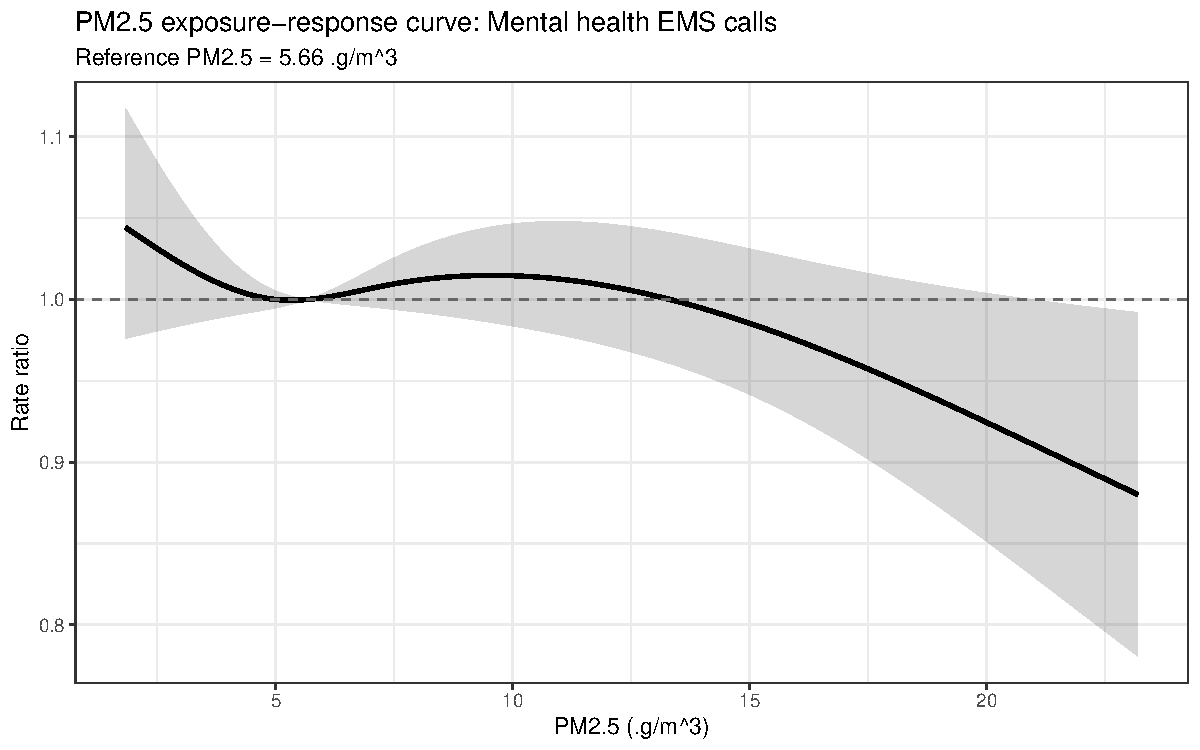
\includegraphics[keepaspectratio]{Preliminary-results_files/figure-latex/unnamed-chunk-9-1.pdf}}

\begin{Shaded}
\begin{Highlighting}[]
\FunctionTok{ggplot}\NormalTok{(curve\_sui, }\FunctionTok{aes}\NormalTok{(}\AttributeTok{x =}\NormalTok{ pm25, }\AttributeTok{y =}\NormalTok{ RR)) }\SpecialCharTok{+}
  \FunctionTok{geom\_ribbon}\NormalTok{(}\FunctionTok{aes}\NormalTok{(}\AttributeTok{ymin =}\NormalTok{ lower, }\AttributeTok{ymax =}\NormalTok{ upper), }\AttributeTok{alpha =} \FloatTok{0.2}\NormalTok{) }\SpecialCharTok{+}
  \FunctionTok{geom\_line}\NormalTok{(}\AttributeTok{linewidth =} \DecValTok{1}\NormalTok{) }\SpecialCharTok{+}
  \FunctionTok{geom\_hline}\NormalTok{(}\AttributeTok{yintercept =} \DecValTok{1}\NormalTok{, }\AttributeTok{linetype =} \DecValTok{2}\NormalTok{, }\AttributeTok{color =} \StringTok{"gray40"}\NormalTok{) }\SpecialCharTok{+}
  \FunctionTok{labs}\NormalTok{(}
    \AttributeTok{title =} \StringTok{"PM2.5 exposure{-}response curve: Suicide{-}related EMS calls"}\NormalTok{,}
    \AttributeTok{subtitle =} \FunctionTok{paste0}\NormalTok{(}\StringTok{"Reference PM2.5 = "}\NormalTok{, }\FunctionTok{round}\NormalTok{(}\FunctionTok{unique}\NormalTok{(curve\_sui}\SpecialCharTok{$}\NormalTok{ref\_value), }\DecValTok{2}\NormalTok{), }\StringTok{" \textbackslash{}u03bcg/m\^{}3"}\NormalTok{),}
    \AttributeTok{x =} \StringTok{"PM2.5 (\textbackslash{}u03bcg/m\^{}3)"}\NormalTok{,}
    \AttributeTok{y =} \StringTok{"Rate ratio"}
\NormalTok{  ) }\SpecialCharTok{+}
  \FunctionTok{theme\_bw}\NormalTok{()}
\end{Highlighting}
\end{Shaded}

\pandocbounded{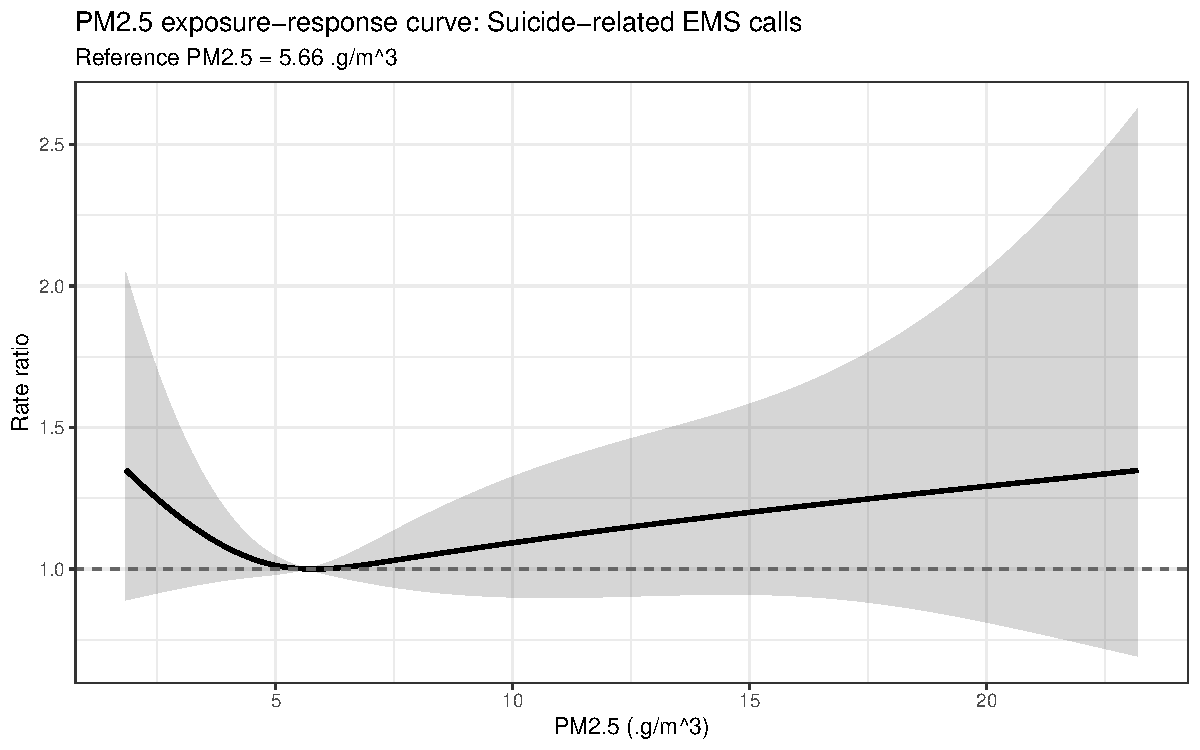
\includegraphics[keepaspectratio]{Preliminary-results_files/figure-latex/unnamed-chunk-10-1.pdf}}

\subsection{Compare linear vs nonlinear PM2.5
specification}\label{compare-linear-vs-nonlinear-pm2.5-specification}

\begin{Shaded}
\begin{Highlighting}[]
\NormalTok{curve\_mh\_linear  }\OtherTok{\textless{}{-}} \FunctionTok{make\_linear\_curve}\NormalTok{(fit\_mh\_linear, df, }\StringTok{"Mental health"}\NormalTok{)}
\NormalTok{curve\_sui\_linear }\OtherTok{\textless{}{-}} \FunctionTok{make\_linear\_curve}\NormalTok{(fit\_sui\_linear, df, }\StringTok{"Suicide"}\NormalTok{)}

\NormalTok{curve\_mh\_nl\_plot  }\OtherTok{\textless{}{-}}\NormalTok{ curve\_mh  }\SpecialCharTok{|\textgreater{}} \FunctionTok{mutate}\NormalTok{(}\AttributeTok{model\_type =} \StringTok{"Nonlinear"}\NormalTok{)}
\NormalTok{curve\_sui\_nl\_plot }\OtherTok{\textless{}{-}}\NormalTok{ curve\_sui }\SpecialCharTok{|\textgreater{}} \FunctionTok{mutate}\NormalTok{(}\AttributeTok{model\_type =} \StringTok{"Nonlinear"}\NormalTok{)}

\NormalTok{curve\_compare\_mh  }\OtherTok{\textless{}{-}} \FunctionTok{bind\_rows}\NormalTok{(curve\_mh\_linear, curve\_mh\_nl\_plot)}
\NormalTok{curve\_compare\_sui }\OtherTok{\textless{}{-}} \FunctionTok{bind\_rows}\NormalTok{(curve\_sui\_linear, curve\_sui\_nl\_plot)}
\end{Highlighting}
\end{Shaded}

\begin{Shaded}
\begin{Highlighting}[]
\FunctionTok{ggplot}\NormalTok{(curve\_compare\_mh, }\FunctionTok{aes}\NormalTok{(}\AttributeTok{x =}\NormalTok{ pm25, }\AttributeTok{y =}\NormalTok{ RR, }\AttributeTok{color =}\NormalTok{ model\_type)) }\SpecialCharTok{+}
  \FunctionTok{geom\_line}\NormalTok{(}\AttributeTok{linewidth =} \DecValTok{1}\NormalTok{) }\SpecialCharTok{+}
  \FunctionTok{geom\_hline}\NormalTok{(}\AttributeTok{yintercept =} \DecValTok{1}\NormalTok{, }\AttributeTok{linetype =} \DecValTok{2}\NormalTok{, }\AttributeTok{color =} \StringTok{"gray40"}\NormalTok{) }\SpecialCharTok{+}
  \FunctionTok{labs}\NormalTok{(}
    \AttributeTok{title =} \StringTok{"Linear vs nonlinear PM2.5 relationship: Mental health calls"}\NormalTok{,}
    \AttributeTok{x =} \StringTok{"PM2.5 (\textbackslash{}u03bcg/m\^{}3)"}\NormalTok{,}
    \AttributeTok{y =} \StringTok{"Rate ratio"}\NormalTok{,}
    \AttributeTok{color =} \StringTok{"Model"}
\NormalTok{  ) }\SpecialCharTok{+}
  \FunctionTok{theme\_bw}\NormalTok{()}
\end{Highlighting}
\end{Shaded}

\pandocbounded{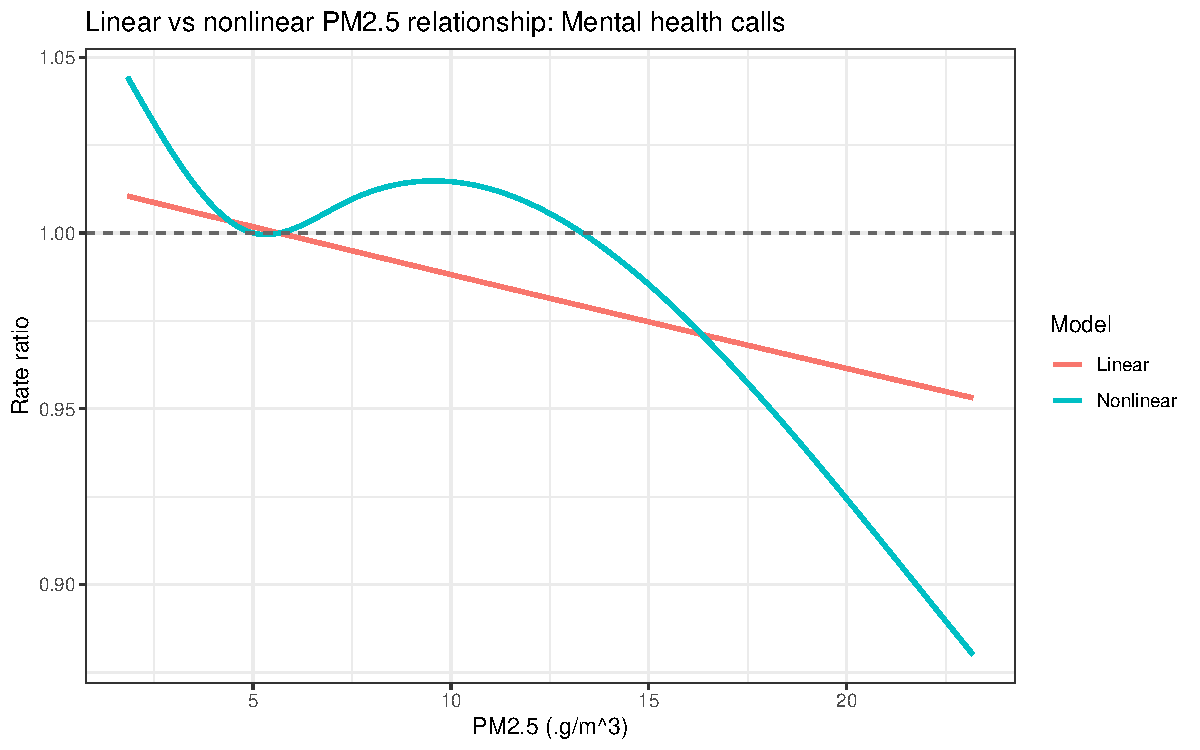
\includegraphics[keepaspectratio]{Preliminary-results_files/figure-latex/unnamed-chunk-12-1.pdf}}

\begin{Shaded}
\begin{Highlighting}[]
\FunctionTok{ggplot}\NormalTok{(curve\_compare\_sui, }\FunctionTok{aes}\NormalTok{(}\AttributeTok{x =}\NormalTok{ pm25, }\AttributeTok{y =}\NormalTok{ RR, }\AttributeTok{color =}\NormalTok{ model\_type)) }\SpecialCharTok{+}
  \FunctionTok{geom\_line}\NormalTok{(}\AttributeTok{linewidth =} \DecValTok{1}\NormalTok{) }\SpecialCharTok{+}
  \FunctionTok{geom\_hline}\NormalTok{(}\AttributeTok{yintercept =} \DecValTok{1}\NormalTok{, }\AttributeTok{linetype =} \DecValTok{2}\NormalTok{, }\AttributeTok{color =} \StringTok{"gray40"}\NormalTok{) }\SpecialCharTok{+}
  \FunctionTok{labs}\NormalTok{(}
    \AttributeTok{title =} \StringTok{"Linear vs nonlinear PM2.5 relationship: Suicide{-}related calls"}\NormalTok{,}
    \AttributeTok{x =} \StringTok{"PM2.5 (\textbackslash{}u03bcg/m\^{}3)"}\NormalTok{,}
    \AttributeTok{y =} \StringTok{"Rate ratio"}\NormalTok{,}
    \AttributeTok{color =} \StringTok{"Model"}
\NormalTok{  ) }\SpecialCharTok{+}
  \FunctionTok{theme\_bw}\NormalTok{()}
\end{Highlighting}
\end{Shaded}

\pandocbounded{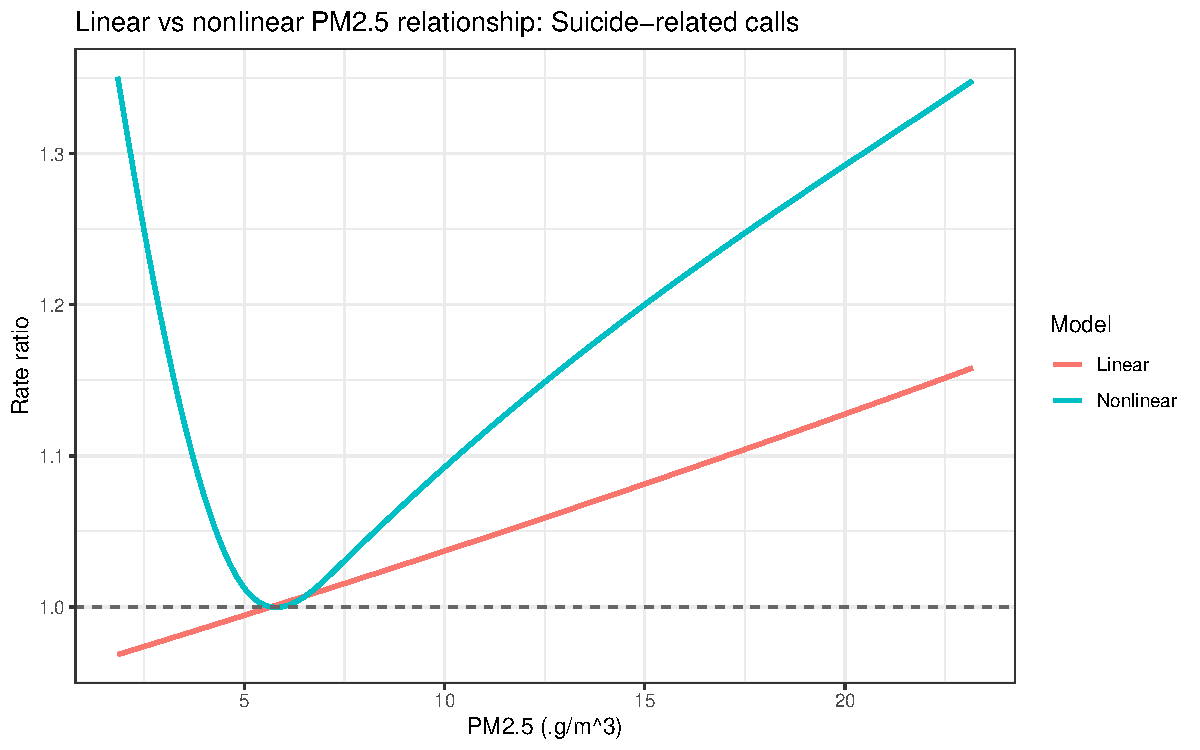
\includegraphics[keepaspectratio]{Preliminary-results_files/figure-latex/unnamed-chunk-13-1.pdf}}

\subsection{Sensitivity analysis 1: PM2.5 spline df =
4}\label{sensitivity-analysis-1-pm2.5-spline-df-4}

\begin{Shaded}
\begin{Highlighting}[]
\NormalTok{fit\_mh\_nonlinear\_df4 }\OtherTok{\textless{}{-}} \FunctionTok{glm}\NormalTok{(}
\NormalTok{  mental\_health }\SpecialCharTok{\textasciitilde{}} \FunctionTok{ns}\NormalTok{(pm25, }\DecValTok{4}\NormalTok{) }\SpecialCharTok{+} \FunctionTok{ns}\NormalTok{(time, }\DecValTok{4}\NormalTok{) }\SpecialCharTok{+} \FunctionTok{ns}\NormalTok{(tmean, }\DecValTok{3}\NormalTok{) }\SpecialCharTok{+}\NormalTok{ is\_weekend }\SpecialCharTok{+}\NormalTok{ precip,}
  \AttributeTok{family =} \FunctionTok{quasipoisson}\NormalTok{(}\AttributeTok{link =} \StringTok{"log"}\NormalTok{),}
  \AttributeTok{data =}\NormalTok{ df}
\NormalTok{)}

\NormalTok{fit\_sui\_nonlinear\_df4 }\OtherTok{\textless{}{-}} \FunctionTok{glm}\NormalTok{(}
\NormalTok{  suicide }\SpecialCharTok{\textasciitilde{}} \FunctionTok{ns}\NormalTok{(pm25, }\DecValTok{4}\NormalTok{) }\SpecialCharTok{+} \FunctionTok{ns}\NormalTok{(time, }\DecValTok{4}\NormalTok{) }\SpecialCharTok{+} \FunctionTok{ns}\NormalTok{(tmean, }\DecValTok{3}\NormalTok{) }\SpecialCharTok{+}\NormalTok{ is\_weekend }\SpecialCharTok{+}\NormalTok{ precip,}
  \AttributeTok{family =} \FunctionTok{quasipoisson}\NormalTok{(}\AttributeTok{link =} \StringTok{"log"}\NormalTok{),}
  \AttributeTok{data =}\NormalTok{ df}
\NormalTok{)}

\NormalTok{curve\_mh\_df4  }\OtherTok{\textless{}{-}} \FunctionTok{make\_er\_curve}\NormalTok{(fit\_mh\_nonlinear\_df4, df, }\StringTok{"Mental health"}\NormalTok{) }\SpecialCharTok{|\textgreater{}} \FunctionTok{mutate}\NormalTok{(}\AttributeTok{df\_pm =} \StringTok{"df = 4"}\NormalTok{)}
\NormalTok{curve\_sui\_df4 }\OtherTok{\textless{}{-}} \FunctionTok{make\_er\_curve}\NormalTok{(fit\_sui\_nonlinear\_df4, df, }\StringTok{"Suicide"}\NormalTok{) }\SpecialCharTok{|\textgreater{}} \FunctionTok{mutate}\NormalTok{(}\AttributeTok{df\_pm =} \StringTok{"df = 4"}\NormalTok{)}

\NormalTok{curve\_mh\_df3  }\OtherTok{\textless{}{-}}\NormalTok{ curve\_mh  }\SpecialCharTok{|\textgreater{}} \FunctionTok{mutate}\NormalTok{(}\AttributeTok{df\_pm =} \StringTok{"df = 3"}\NormalTok{)}
\NormalTok{curve\_sui\_df3 }\OtherTok{\textless{}{-}}\NormalTok{ curve\_sui }\SpecialCharTok{|\textgreater{}} \FunctionTok{mutate}\NormalTok{(}\AttributeTok{df\_pm =} \StringTok{"df = 3"}\NormalTok{)}

\NormalTok{curve\_mh\_sens  }\OtherTok{\textless{}{-}} \FunctionTok{bind\_rows}\NormalTok{(curve\_mh\_df3, curve\_mh\_df4)}
\NormalTok{curve\_sui\_sens }\OtherTok{\textless{}{-}} \FunctionTok{bind\_rows}\NormalTok{(curve\_sui\_df3, curve\_sui\_df4)}
\end{Highlighting}
\end{Shaded}

\begin{Shaded}
\begin{Highlighting}[]
\FunctionTok{ggplot}\NormalTok{(curve\_mh\_sens, }\FunctionTok{aes}\NormalTok{(pm25, RR, }\AttributeTok{color =}\NormalTok{ df\_pm)) }\SpecialCharTok{+}
  \FunctionTok{geom\_line}\NormalTok{(}\AttributeTok{linewidth =} \DecValTok{1}\NormalTok{) }\SpecialCharTok{+}
  \FunctionTok{geom\_hline}\NormalTok{(}\AttributeTok{yintercept =} \DecValTok{1}\NormalTok{, }\AttributeTok{linetype =} \DecValTok{2}\NormalTok{) }\SpecialCharTok{+}
  \FunctionTok{labs}\NormalTok{(}
    \AttributeTok{title =} \StringTok{"Sensitivity to PM2.5 spline df: Mental health"}\NormalTok{,}
    \AttributeTok{x =} \StringTok{"PM2.5 (\textbackslash{}u03bcg/m\^{}3)"}\NormalTok{,}
    \AttributeTok{y =} \StringTok{"Rate ratio"}\NormalTok{,}
    \AttributeTok{color =} \StringTok{"PM2.5 spline"}
\NormalTok{  ) }\SpecialCharTok{+}
  \FunctionTok{theme\_bw}\NormalTok{()}
\end{Highlighting}
\end{Shaded}

\pandocbounded{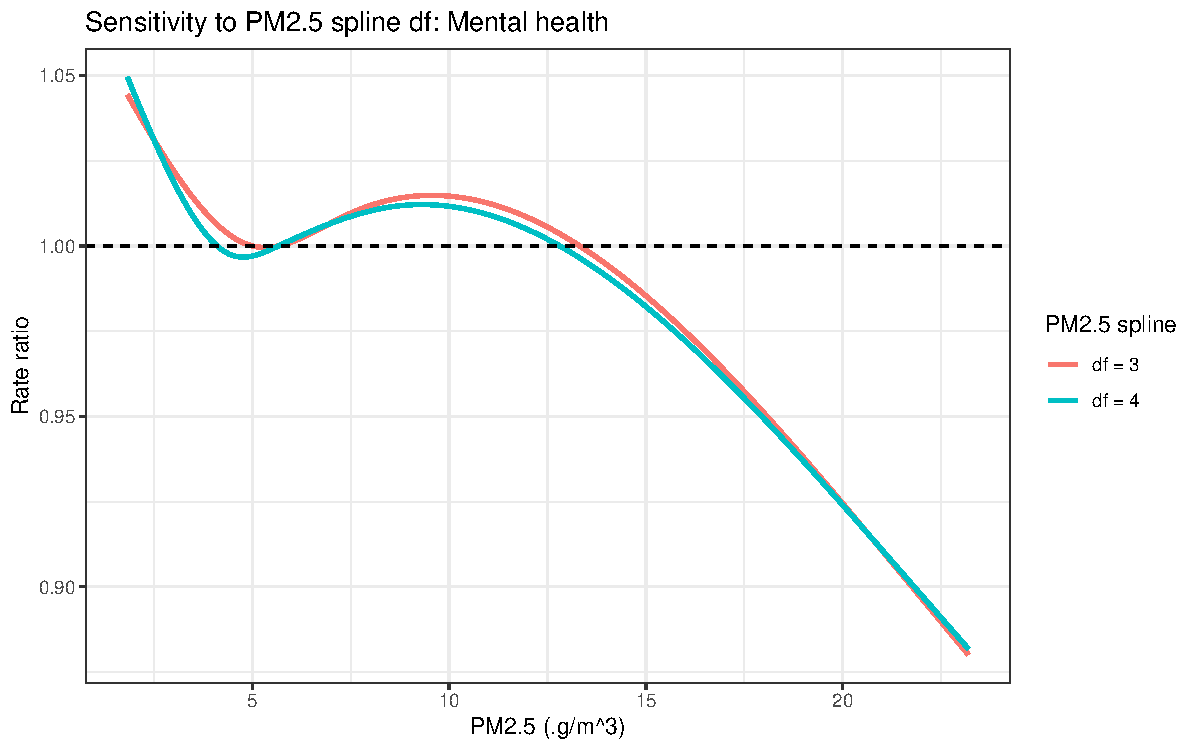
\includegraphics[keepaspectratio]{Preliminary-results_files/figure-latex/unnamed-chunk-15-1.pdf}}

\begin{Shaded}
\begin{Highlighting}[]
\FunctionTok{ggplot}\NormalTok{(curve\_sui\_sens, }\FunctionTok{aes}\NormalTok{(pm25, RR, }\AttributeTok{color =}\NormalTok{ df\_pm)) }\SpecialCharTok{+}
  \FunctionTok{geom\_line}\NormalTok{(}\AttributeTok{linewidth =} \DecValTok{1}\NormalTok{) }\SpecialCharTok{+}
  \FunctionTok{geom\_hline}\NormalTok{(}\AttributeTok{yintercept =} \DecValTok{1}\NormalTok{, }\AttributeTok{linetype =} \DecValTok{2}\NormalTok{) }\SpecialCharTok{+}
  \FunctionTok{labs}\NormalTok{(}
    \AttributeTok{title =} \StringTok{"Sensitivity to PM2.5 spline df: Suicide"}\NormalTok{,}
    \AttributeTok{x =} \StringTok{"PM2.5 (\textbackslash{}u03bcg/m\^{}3)"}\NormalTok{,}
    \AttributeTok{y =} \StringTok{"Rate ratio"}\NormalTok{,}
    \AttributeTok{color =} \StringTok{"PM2.5 spline"}
\NormalTok{  ) }\SpecialCharTok{+}
  \FunctionTok{theme\_bw}\NormalTok{()}
\end{Highlighting}
\end{Shaded}

\pandocbounded{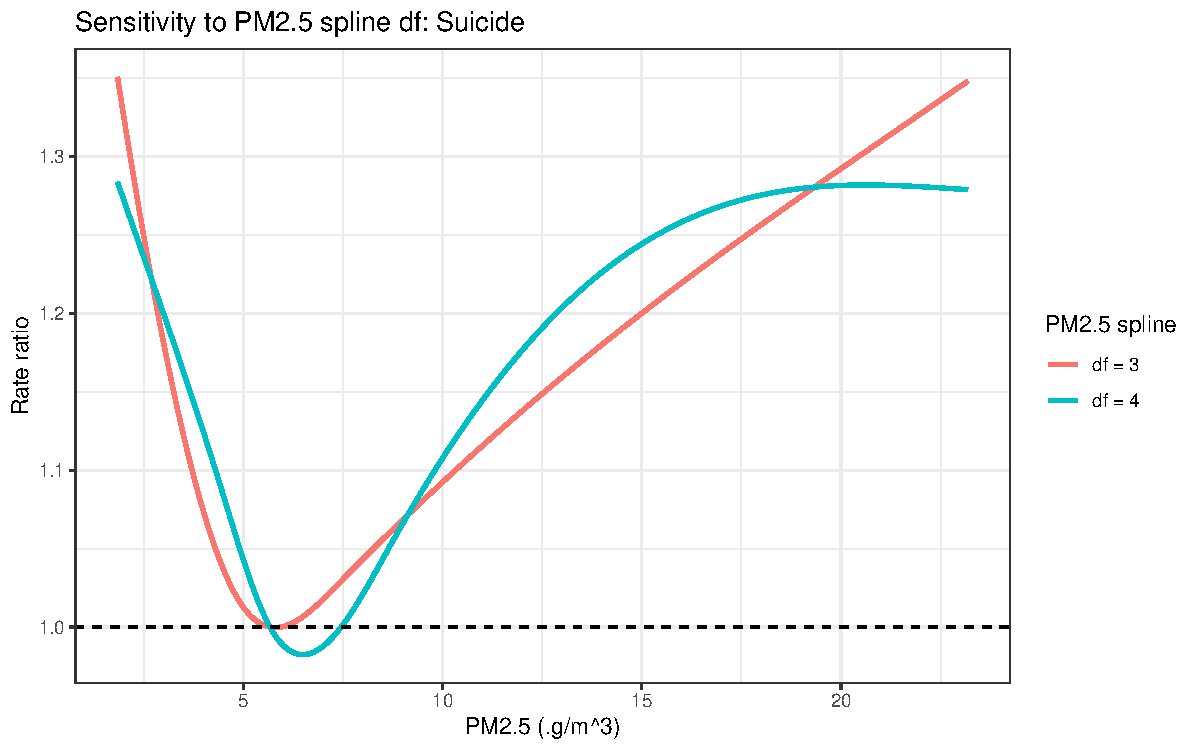
\includegraphics[keepaspectratio]{Preliminary-results_files/figure-latex/unnamed-chunk-16-1.pdf}}

\subsection{Sensitivity analysis 2: exclude high PM2.5
days}\label{sensitivity-analysis-2-exclude-high-pm2.5-days}

\begin{Shaded}
\begin{Highlighting}[]
\NormalTok{pm95 }\OtherTok{\textless{}{-}} \FunctionTok{quantile}\NormalTok{(df}\SpecialCharTok{$}\NormalTok{pm25, }\FloatTok{0.95}\NormalTok{, }\AttributeTok{na.rm =} \ConstantTok{TRUE}\NormalTok{)}

\NormalTok{df\_no\_high }\OtherTok{\textless{}{-}}\NormalTok{ df }\SpecialCharTok{|\textgreater{}} \FunctionTok{filter}\NormalTok{(pm25 }\SpecialCharTok{\textless{}=}\NormalTok{ pm95)}

\NormalTok{fit\_mh\_no\_high }\OtherTok{\textless{}{-}} \FunctionTok{glm}\NormalTok{(}
\NormalTok{  mental\_health }\SpecialCharTok{\textasciitilde{}} \FunctionTok{ns}\NormalTok{(pm25, }\DecValTok{3}\NormalTok{) }\SpecialCharTok{+} \FunctionTok{ns}\NormalTok{(time, }\DecValTok{4}\NormalTok{) }\SpecialCharTok{+} \FunctionTok{ns}\NormalTok{(tmean, }\DecValTok{3}\NormalTok{) }\SpecialCharTok{+}\NormalTok{ is\_weekend }\SpecialCharTok{+}\NormalTok{ precip,}
  \AttributeTok{family =} \FunctionTok{quasipoisson}\NormalTok{(}\AttributeTok{link =} \StringTok{"log"}\NormalTok{),}
  \AttributeTok{data =}\NormalTok{ df\_no\_high}
\NormalTok{)}

\NormalTok{fit\_sui\_no\_high }\OtherTok{\textless{}{-}} \FunctionTok{glm}\NormalTok{(}
\NormalTok{  suicide }\SpecialCharTok{\textasciitilde{}} \FunctionTok{ns}\NormalTok{(pm25, }\DecValTok{3}\NormalTok{) }\SpecialCharTok{+} \FunctionTok{ns}\NormalTok{(time, }\DecValTok{4}\NormalTok{) }\SpecialCharTok{+} \FunctionTok{ns}\NormalTok{(tmean, }\DecValTok{3}\NormalTok{) }\SpecialCharTok{+}\NormalTok{ is\_weekend }\SpecialCharTok{+}\NormalTok{ precip,}
  \AttributeTok{family =} \FunctionTok{quasipoisson}\NormalTok{(}\AttributeTok{link =} \StringTok{"log"}\NormalTok{),}
  \AttributeTok{data =}\NormalTok{ df\_no\_high}
\NormalTok{)}

\NormalTok{curve\_mh\_no\_high }\OtherTok{\textless{}{-}} \FunctionTok{make\_er\_curve}\NormalTok{(fit\_mh\_no\_high, df\_no\_high, }\StringTok{"Mental health"}\NormalTok{) }\SpecialCharTok{|\textgreater{}}
  \FunctionTok{mutate}\NormalTok{(}\AttributeTok{sample =} \StringTok{"Exclude \textgreater{}95th percentile"}\NormalTok{)}

\NormalTok{curve\_sui\_no\_high }\OtherTok{\textless{}{-}} \FunctionTok{make\_er\_curve}\NormalTok{(fit\_sui\_no\_high, df\_no\_high, }\StringTok{"Suicide"}\NormalTok{) }\SpecialCharTok{|\textgreater{}}
  \FunctionTok{mutate}\NormalTok{(}\AttributeTok{sample =} \StringTok{"Exclude \textgreater{}95th percentile"}\NormalTok{)}

\NormalTok{curve\_mh\_main }\OtherTok{\textless{}{-}}\NormalTok{ curve\_mh }\SpecialCharTok{|\textgreater{}} \FunctionTok{mutate}\NormalTok{(}\AttributeTok{sample =} \StringTok{"Main sample"}\NormalTok{)}
\NormalTok{curve\_sui\_main }\OtherTok{\textless{}{-}}\NormalTok{ curve\_sui }\SpecialCharTok{|\textgreater{}} \FunctionTok{mutate}\NormalTok{(}\AttributeTok{sample =} \StringTok{"Main sample"}\NormalTok{)}
\end{Highlighting}
\end{Shaded}

\begin{Shaded}
\begin{Highlighting}[]
\FunctionTok{ggplot}\NormalTok{(}\FunctionTok{bind\_rows}\NormalTok{(curve\_mh\_main, curve\_mh\_no\_high), }\FunctionTok{aes}\NormalTok{(pm25, RR, }\AttributeTok{color =}\NormalTok{ sample)) }\SpecialCharTok{+}
  \FunctionTok{geom\_line}\NormalTok{(}\AttributeTok{linewidth =} \DecValTok{1}\NormalTok{) }\SpecialCharTok{+}
  \FunctionTok{geom\_hline}\NormalTok{(}\AttributeTok{yintercept =} \DecValTok{1}\NormalTok{, }\AttributeTok{linetype =} \DecValTok{2}\NormalTok{) }\SpecialCharTok{+}
  \FunctionTok{labs}\NormalTok{(}
    \AttributeTok{title =} \StringTok{"Sensitivity to extreme PM2.5 days: Mental health"}\NormalTok{,}
    \AttributeTok{x =} \StringTok{"PM2.5 (\textbackslash{}u03bcg/m\^{}3)"}\NormalTok{,}
    \AttributeTok{y =} \StringTok{"Rate ratio"}
\NormalTok{  ) }\SpecialCharTok{+}
  \FunctionTok{theme\_bw}\NormalTok{()}
\end{Highlighting}
\end{Shaded}

\pandocbounded{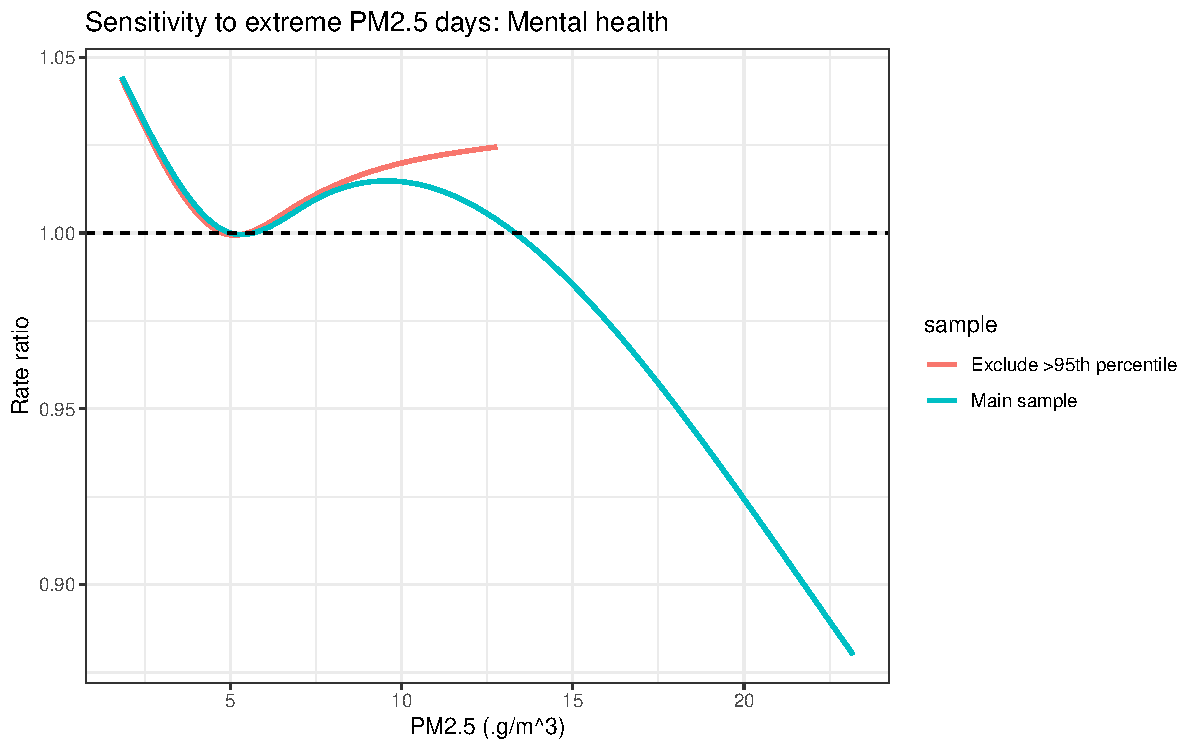
\includegraphics[keepaspectratio]{Preliminary-results_files/figure-latex/unnamed-chunk-18-1.pdf}}

\begin{Shaded}
\begin{Highlighting}[]
\FunctionTok{ggplot}\NormalTok{(}\FunctionTok{bind\_rows}\NormalTok{(curve\_sui\_main, curve\_sui\_no\_high), }\FunctionTok{aes}\NormalTok{(pm25, RR, }\AttributeTok{color =}\NormalTok{ sample)) }\SpecialCharTok{+}
  \FunctionTok{geom\_line}\NormalTok{(}\AttributeTok{linewidth =} \DecValTok{1}\NormalTok{) }\SpecialCharTok{+}
  \FunctionTok{geom\_hline}\NormalTok{(}\AttributeTok{yintercept =} \DecValTok{1}\NormalTok{, }\AttributeTok{linetype =} \DecValTok{2}\NormalTok{) }\SpecialCharTok{+}
  \FunctionTok{labs}\NormalTok{(}
    \AttributeTok{title =} \StringTok{"Sensitivity to extreme PM2.5 days: Suicide"}\NormalTok{,}
    \AttributeTok{x =} \StringTok{"PM2.5 (\textbackslash{}u03bcg/m\^{}3)"}\NormalTok{,}
    \AttributeTok{y =} \StringTok{"Rate ratio"}
\NormalTok{  ) }\SpecialCharTok{+}
  \FunctionTok{theme\_bw}\NormalTok{()}
\end{Highlighting}
\end{Shaded}

\pandocbounded{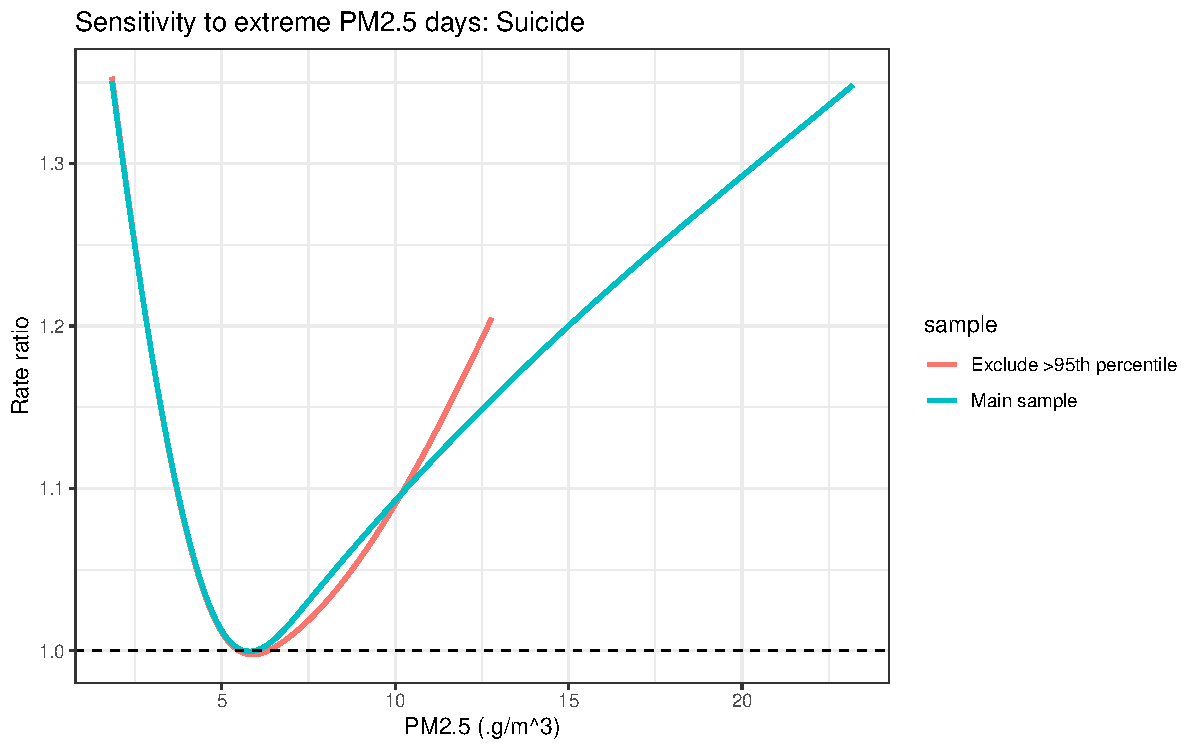
\includegraphics[keepaspectratio]{Preliminary-results_files/figure-latex/unnamed-chunk-19-1.pdf}}

\subsection{Sensitivity analysis 3: alternative time-trend df
(3--6)}\label{sensitivity-analysis-3-alternative-time-trend-df-36}

\begin{Shaded}
\begin{Highlighting}[]
\NormalTok{fit\_time\_sensitivity }\OtherTok{\textless{}{-}} \ControlFlowTok{function}\NormalTok{(outcome, time\_df, data) \{}
\NormalTok{  form }\OtherTok{\textless{}{-}} \FunctionTok{as.formula}\NormalTok{(}
    \FunctionTok{paste0}\NormalTok{(outcome,}
           \StringTok{" \textasciitilde{} ns(pm25, 3) + ns(time, "}\NormalTok{, time\_df, }\StringTok{") + ns(tmean, 3) + is\_weekend + precip"}\NormalTok{)}
\NormalTok{  )}

  \FunctionTok{glm}\NormalTok{(form, }\AttributeTok{family =} \FunctionTok{quasipoisson}\NormalTok{(}\AttributeTok{link =} \StringTok{"log"}\NormalTok{), }\AttributeTok{data =}\NormalTok{ data)}
\NormalTok{\}}

\NormalTok{time\_df\_results\_mh }\OtherTok{\textless{}{-}} \FunctionTok{map\_df}\NormalTok{(}\DecValTok{3}\SpecialCharTok{:}\DecValTok{6}\NormalTok{, }\ControlFlowTok{function}\NormalTok{(k) \{}
\NormalTok{  mod }\OtherTok{\textless{}{-}} \FunctionTok{fit\_time\_sensitivity}\NormalTok{(}\StringTok{"mental\_health"}\NormalTok{, k, df)}
\NormalTok{  curve }\OtherTok{\textless{}{-}} \FunctionTok{make\_er\_curve}\NormalTok{(mod, df, }\StringTok{"Mental health"}\NormalTok{)}
\NormalTok{  curve}\SpecialCharTok{$}\NormalTok{time\_df }\OtherTok{\textless{}{-}} \FunctionTok{paste0}\NormalTok{(}\StringTok{"time df = "}\NormalTok{, k)}
\NormalTok{  curve}
\NormalTok{\})}

\NormalTok{time\_df\_results\_sui }\OtherTok{\textless{}{-}} \FunctionTok{map\_df}\NormalTok{(}\DecValTok{3}\SpecialCharTok{:}\DecValTok{6}\NormalTok{, }\ControlFlowTok{function}\NormalTok{(k) \{}
\NormalTok{  mod }\OtherTok{\textless{}{-}} \FunctionTok{fit\_time\_sensitivity}\NormalTok{(}\StringTok{"suicide"}\NormalTok{, k, df)}
\NormalTok{  curve }\OtherTok{\textless{}{-}} \FunctionTok{make\_er\_curve}\NormalTok{(mod, df, }\StringTok{"Suicide"}\NormalTok{)}
\NormalTok{  curve}\SpecialCharTok{$}\NormalTok{time\_df }\OtherTok{\textless{}{-}} \FunctionTok{paste0}\NormalTok{(}\StringTok{"time df = "}\NormalTok{, k)}
\NormalTok{  curve}
\NormalTok{\})}
\end{Highlighting}
\end{Shaded}

\begin{Shaded}
\begin{Highlighting}[]
\FunctionTok{ggplot}\NormalTok{(time\_df\_results\_mh, }\FunctionTok{aes}\NormalTok{(pm25, RR, }\AttributeTok{color =}\NormalTok{ time\_df)) }\SpecialCharTok{+}
  \FunctionTok{geom\_line}\NormalTok{(}\AttributeTok{linewidth =} \DecValTok{1}\NormalTok{) }\SpecialCharTok{+}
  \FunctionTok{geom\_hline}\NormalTok{(}\AttributeTok{yintercept =} \DecValTok{1}\NormalTok{, }\AttributeTok{linetype =} \DecValTok{2}\NormalTok{) }\SpecialCharTok{+}
  \FunctionTok{labs}\NormalTok{(}
    \AttributeTok{title =} \StringTok{"Sensitivity to time{-}trend df: Mental health"}\NormalTok{,}
    \AttributeTok{x =} \StringTok{"PM2.5 (\textbackslash{}u03bcg/m\^{}3)"}\NormalTok{,}
    \AttributeTok{y =} \StringTok{"Rate ratio"}\NormalTok{,}
    \AttributeTok{color =} \StringTok{"Time spline"}
\NormalTok{  ) }\SpecialCharTok{+}
  \FunctionTok{theme\_bw}\NormalTok{()}
\end{Highlighting}
\end{Shaded}

\pandocbounded{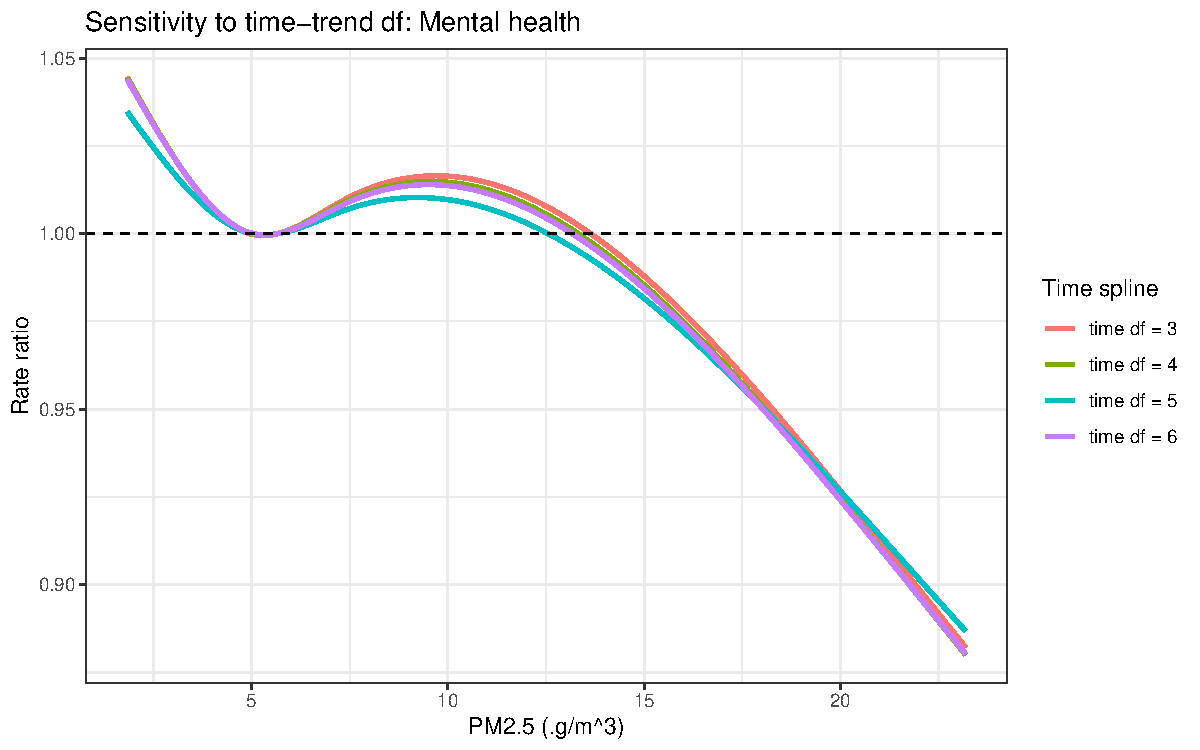
\includegraphics[keepaspectratio]{Preliminary-results_files/figure-latex/unnamed-chunk-21-1.pdf}}

\begin{Shaded}
\begin{Highlighting}[]
\FunctionTok{ggplot}\NormalTok{(time\_df\_results\_sui, }\FunctionTok{aes}\NormalTok{(pm25, RR, }\AttributeTok{color =}\NormalTok{ time\_df)) }\SpecialCharTok{+}
  \FunctionTok{geom\_line}\NormalTok{(}\AttributeTok{linewidth =} \DecValTok{1}\NormalTok{) }\SpecialCharTok{+}
  \FunctionTok{geom\_hline}\NormalTok{(}\AttributeTok{yintercept =} \DecValTok{1}\NormalTok{, }\AttributeTok{linetype =} \DecValTok{2}\NormalTok{) }\SpecialCharTok{+}
  \FunctionTok{labs}\NormalTok{(}
    \AttributeTok{title =} \StringTok{"Sensitivity to time{-}trend df: Suicide"}\NormalTok{,}
    \AttributeTok{x =} \StringTok{"PM2.5 (\textbackslash{}u03bcg/m\^{}3)"}\NormalTok{,}
    \AttributeTok{y =} \StringTok{"Rate ratio"}\NormalTok{,}
    \AttributeTok{color =} \StringTok{"Time spline"}
\NormalTok{  ) }\SpecialCharTok{+}
  \FunctionTok{theme\_bw}\NormalTok{()}
\end{Highlighting}
\end{Shaded}

\pandocbounded{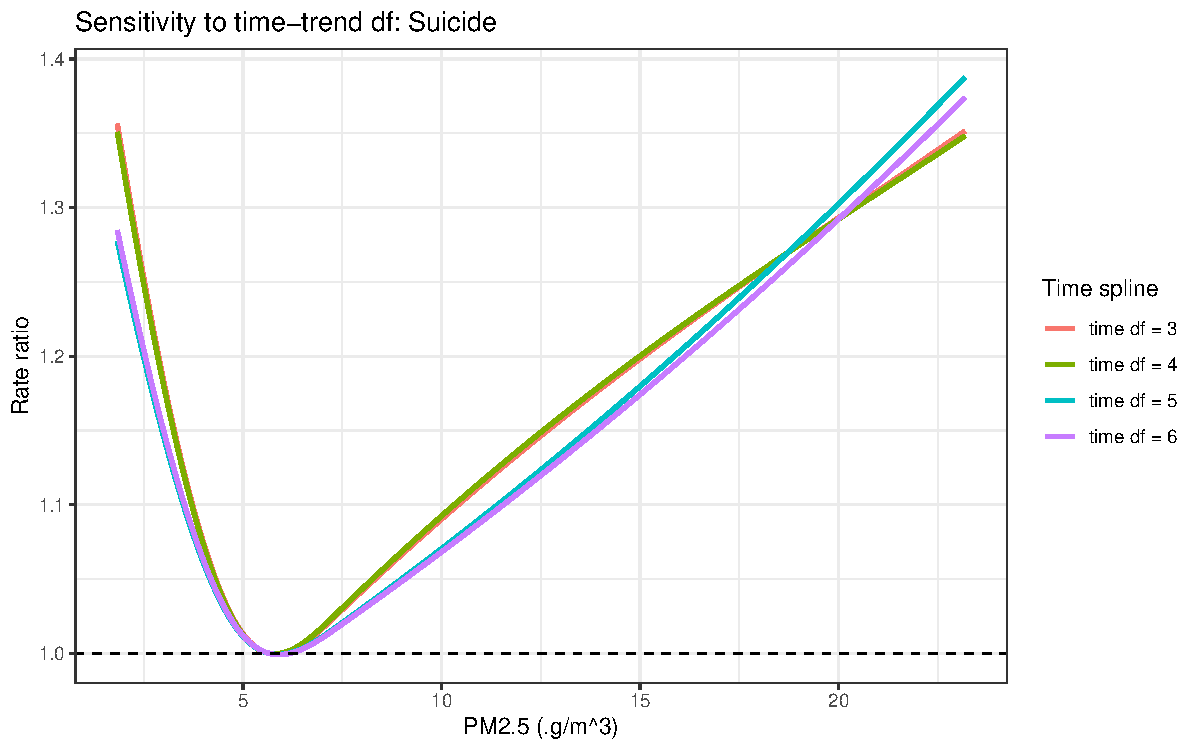
\includegraphics[keepaspectratio]{Preliminary-results_files/figure-latex/unnamed-chunk-22-1.pdf}}

\subsection{Sensitivity analysis 4: nonlinear
precipitation}\label{sensitivity-analysis-4-nonlinear-precipitation}

\begin{Shaded}
\begin{Highlighting}[]
\NormalTok{fit\_mh\_nl\_precip }\OtherTok{\textless{}{-}} \FunctionTok{glm}\NormalTok{(}
\NormalTok{  mental\_health }\SpecialCharTok{\textasciitilde{}} \FunctionTok{ns}\NormalTok{(pm25, }\DecValTok{3}\NormalTok{) }\SpecialCharTok{+} \FunctionTok{ns}\NormalTok{(time, }\DecValTok{4}\NormalTok{) }\SpecialCharTok{+} \FunctionTok{ns}\NormalTok{(tmean, }\DecValTok{3}\NormalTok{) }\SpecialCharTok{+}\NormalTok{ is\_weekend }\SpecialCharTok{+} \FunctionTok{ns}\NormalTok{(precip, }\DecValTok{3}\NormalTok{),}
  \AttributeTok{family =} \FunctionTok{quasipoisson}\NormalTok{(}\AttributeTok{link =} \StringTok{"log"}\NormalTok{),}
  \AttributeTok{data =}\NormalTok{ df}
\NormalTok{)}

\NormalTok{fit\_sui\_nl\_precip }\OtherTok{\textless{}{-}} \FunctionTok{glm}\NormalTok{(}
\NormalTok{  suicide }\SpecialCharTok{\textasciitilde{}} \FunctionTok{ns}\NormalTok{(pm25, }\DecValTok{3}\NormalTok{) }\SpecialCharTok{+} \FunctionTok{ns}\NormalTok{(time, }\DecValTok{4}\NormalTok{) }\SpecialCharTok{+} \FunctionTok{ns}\NormalTok{(tmean, }\DecValTok{3}\NormalTok{) }\SpecialCharTok{+}\NormalTok{ is\_weekend }\SpecialCharTok{+} \FunctionTok{ns}\NormalTok{(precip, }\DecValTok{3}\NormalTok{),}
  \AttributeTok{family =} \FunctionTok{quasipoisson}\NormalTok{(}\AttributeTok{link =} \StringTok{"log"}\NormalTok{),}
  \AttributeTok{data =}\NormalTok{ df}
\NormalTok{)}

\NormalTok{curve\_mh\_nl\_precip }\OtherTok{\textless{}{-}} \FunctionTok{make\_er\_curve}\NormalTok{(fit\_mh\_nl\_precip, df, }\StringTok{"Mental health"}\NormalTok{) }\SpecialCharTok{|\textgreater{}}
  \FunctionTok{mutate}\NormalTok{(}\AttributeTok{model =} \StringTok{"Nonlinear precip"}\NormalTok{)}

\NormalTok{curve\_sui\_nl\_precip }\OtherTok{\textless{}{-}} \FunctionTok{make\_er\_curve}\NormalTok{(fit\_sui\_nl\_precip, df, }\StringTok{"Suicide"}\NormalTok{) }\SpecialCharTok{|\textgreater{}}
  \FunctionTok{mutate}\NormalTok{(}\AttributeTok{model =} \StringTok{"Nonlinear precip"}\NormalTok{)}

\NormalTok{curve\_mh\_main2 }\OtherTok{\textless{}{-}}\NormalTok{ curve\_mh }\SpecialCharTok{|\textgreater{}} \FunctionTok{mutate}\NormalTok{(}\AttributeTok{model =} \StringTok{"Linear precip"}\NormalTok{)}
\NormalTok{curve\_sui\_main2 }\OtherTok{\textless{}{-}}\NormalTok{ curve\_sui }\SpecialCharTok{|\textgreater{}} \FunctionTok{mutate}\NormalTok{(}\AttributeTok{model =} \StringTok{"Linear precip"}\NormalTok{)}
\end{Highlighting}
\end{Shaded}

\begin{Shaded}
\begin{Highlighting}[]
\FunctionTok{ggplot}\NormalTok{(}\FunctionTok{bind\_rows}\NormalTok{(curve\_mh\_main2, curve\_mh\_nl\_precip), }\FunctionTok{aes}\NormalTok{(pm25, RR, }\AttributeTok{color =}\NormalTok{ model)) }\SpecialCharTok{+}
  \FunctionTok{geom\_line}\NormalTok{(}\AttributeTok{linewidth =} \DecValTok{1}\NormalTok{) }\SpecialCharTok{+}
  \FunctionTok{geom\_hline}\NormalTok{(}\AttributeTok{yintercept =} \DecValTok{1}\NormalTok{, }\AttributeTok{linetype =} \DecValTok{2}\NormalTok{) }\SpecialCharTok{+}
  \FunctionTok{labs}\NormalTok{(}
    \AttributeTok{title =} \StringTok{"Sensitivity to precipitation functional form: Mental health"}\NormalTok{,}
    \AttributeTok{x =} \StringTok{"PM2.5 (\textbackslash{}u03bcg/m\^{}3)"}\NormalTok{,}
    \AttributeTok{y =} \StringTok{"Rate ratio"}
\NormalTok{  ) }\SpecialCharTok{+}
  \FunctionTok{theme\_bw}\NormalTok{()}
\end{Highlighting}
\end{Shaded}

\pandocbounded{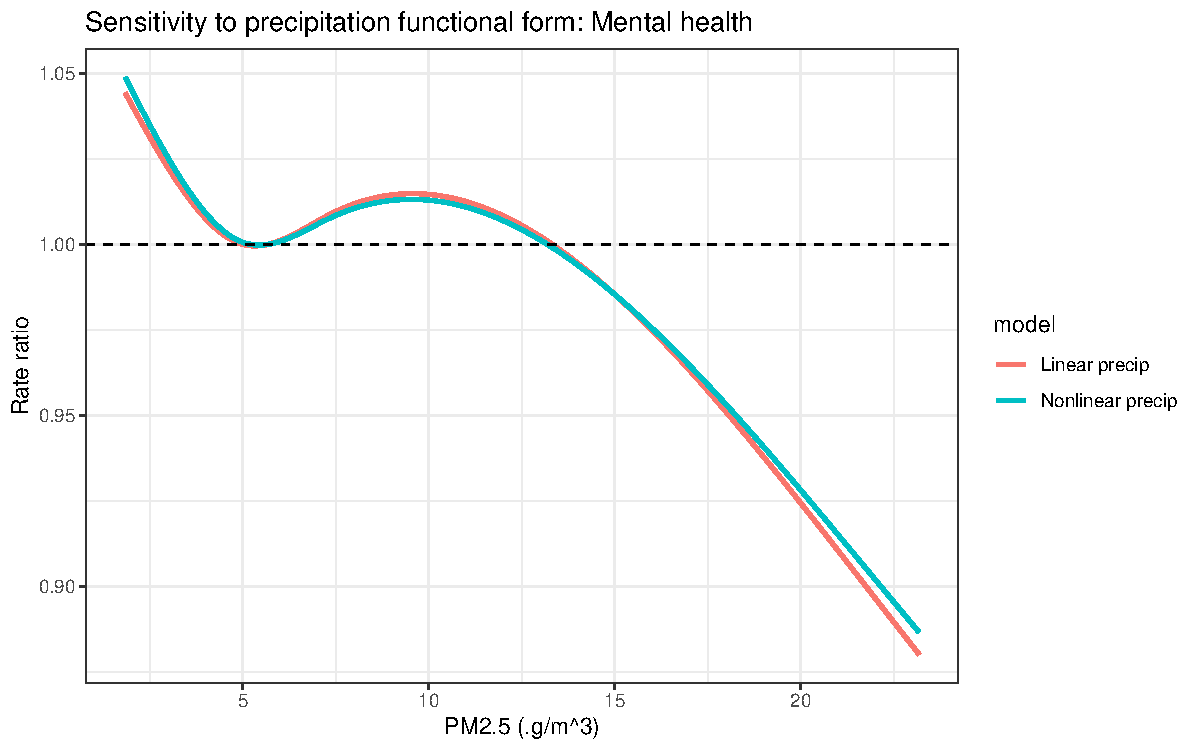
\includegraphics[keepaspectratio]{Preliminary-results_files/figure-latex/unnamed-chunk-24-1.pdf}}

\begin{Shaded}
\begin{Highlighting}[]
\FunctionTok{ggplot}\NormalTok{(}\FunctionTok{bind\_rows}\NormalTok{(curve\_sui\_main2, curve\_sui\_nl\_precip), }\FunctionTok{aes}\NormalTok{(pm25, RR, }\AttributeTok{color =}\NormalTok{ model)) }\SpecialCharTok{+}
  \FunctionTok{geom\_line}\NormalTok{(}\AttributeTok{linewidth =} \DecValTok{1}\NormalTok{) }\SpecialCharTok{+}
  \FunctionTok{geom\_hline}\NormalTok{(}\AttributeTok{yintercept =} \DecValTok{1}\NormalTok{, }\AttributeTok{linetype =} \DecValTok{2}\NormalTok{) }\SpecialCharTok{+}
  \FunctionTok{labs}\NormalTok{(}
    \AttributeTok{title =} \StringTok{"Sensitivity to precipitation functional form: Suicide"}\NormalTok{,}
    \AttributeTok{x =} \StringTok{"PM2.5 (\textbackslash{}u03bcg/m\^{}3)"}\NormalTok{,}
    \AttributeTok{y =} \StringTok{"Rate ratio"}
\NormalTok{  ) }\SpecialCharTok{+}
  \FunctionTok{theme\_bw}\NormalTok{()}
\end{Highlighting}
\end{Shaded}

\pandocbounded{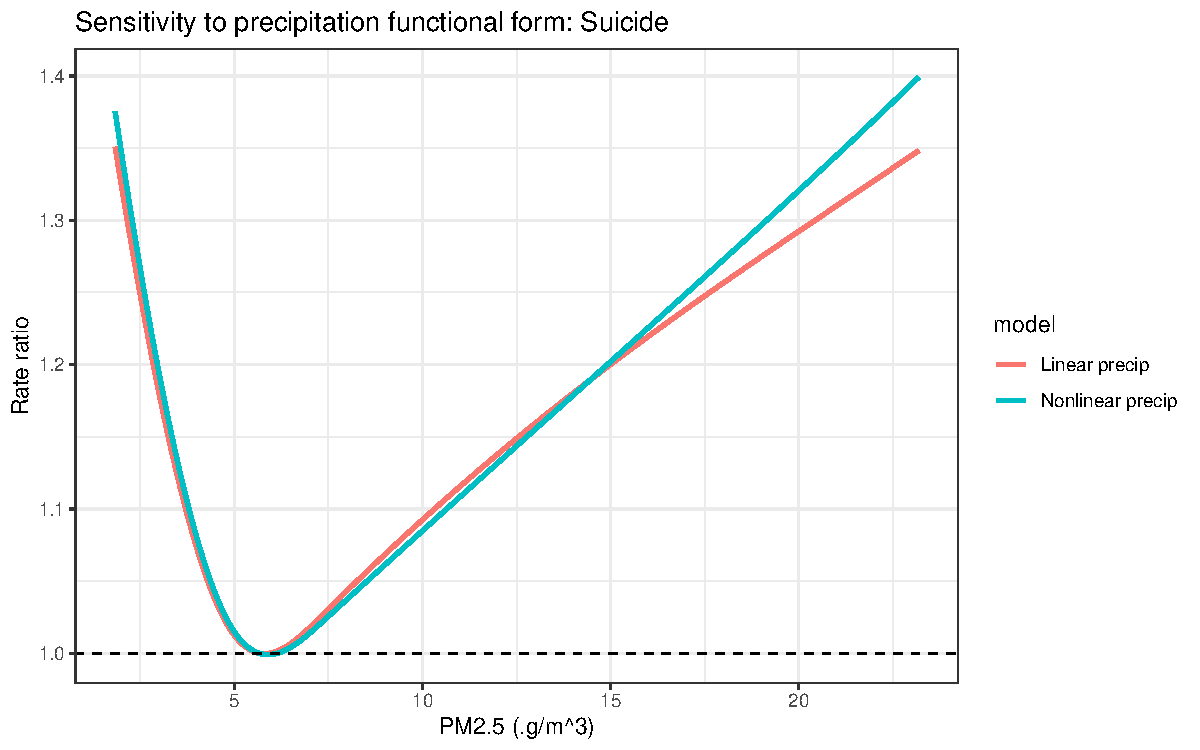
\includegraphics[keepaspectratio]{Preliminary-results_files/figure-latex/unnamed-chunk-25-1.pdf}}

\subsection{Results section outline}\label{results-section-outline}

\subsubsection{Nonlinear exposure--response
analysis}\label{nonlinear-exposureresponse-analysis}

I fit quasi-Poisson time-series models with a natural spline for
same-day PM2.5, adjusting for seasonal trend, temperature, weekend, and
precipitation, and compared the nonlinear PM2.5 specification with the
corresponding linear model for both outcomes.

\subsubsection{Mental health EMS calls}\label{mental-health-ems-calls}

For mental health EMS calls, the adjusted nonlinear exposure--response
curve was close to null over most of the observed PM2.5 range. The curve
showed only a modest mid-range rise followed by a gradual decline at
higher concentrations, with no clear threshold or strong positive
nonlinear pattern. Confidence intervals widened at the tails, especially
at higher PM2.5 levels.

\subsubsection{Suicide-related EMS
calls}\label{suicide-related-ems-calls}

For suicide-related EMS calls, the nonlinear curve decreased toward the
reference value at lower PM2.5 concentrations and then gradually
increased at higher concentrations. However, confidence intervals were
wide throughout, particularly at the upper end, indicating substantial
uncertainty.

\subsubsection{Comparison of linear and nonlinear PM2.5
specifications}\label{comparison-of-linear-and-nonlinear-pm2.5-specifications}

For mental health EMS calls, the linear and nonlinear models gave
similar overall conclusions, with no strong positive association. For
suicide-related EMS calls, both models suggested higher risk at higher
PM2.5 levels, but the nonlinear model showed more curvature.

\subsubsection{Sensitivity analyses}\label{sensitivity-analyses}

For mental health EMS calls, the curve was highly stable across
sensitivity analyses, including alternative PM2.5 spline degrees of
freedom, time-trend adjustment, and precipitation specification.
Excluding PM2.5 values above the 95th percentile reduced the downward
trend at the highest concentrations, suggesting some influence of
extreme exposure days.

For suicide-related EMS calls, the overall pattern was also similar
across sensitivity analyses, with a dip near the reference value
followed by an upward trend at higher PM2.5 levels, although the exact
shape was somewhat less stable than for mental health EMS calls.

\section{Quasi-Poisson Time Series GLM (Yiming
Cao)}\label{quasi-poisson-time-series-glm-yiming-cao}

\subsection{Model fitting}\label{model-fitting}

Using the same data loaded above. The main model keeps PM2.5 as a linear
exposure term --- the goal here is to estimate the rate ratio per 10
μg/m³ increase, adjusting for seasonal trend, temperature, weekend
effect, and precipitation.

\begin{Shaded}
\begin{Highlighting}[]
\FunctionTok{library}\NormalTok{(splines)}

\CommentTok{\# time variable as days since Jan 1}
\NormalTok{df}\SpecialCharTok{$}\NormalTok{time\_days }\OtherTok{\textless{}{-}} \FunctionTok{as.numeric}\NormalTok{(df}\SpecialCharTok{$}\NormalTok{date }\SpecialCharTok{{-}} \FunctionTok{min}\NormalTok{(df}\SpecialCharTok{$}\NormalTok{date))}

\CommentTok{\# mental health model}
\NormalTok{fit\_qp\_mh }\OtherTok{\textless{}{-}} \FunctionTok{glm}\NormalTok{(mental\_health }\SpecialCharTok{\textasciitilde{}}\NormalTok{ pm25 }\SpecialCharTok{+} \FunctionTok{ns}\NormalTok{(time\_days, }\DecValTok{4}\NormalTok{) }\SpecialCharTok{+} \FunctionTok{ns}\NormalTok{(tmean, }\DecValTok{3}\NormalTok{) }\SpecialCharTok{+}
\NormalTok{                    is\_weekend }\SpecialCharTok{+}\NormalTok{ precip,}
                  \AttributeTok{family =} \FunctionTok{quasipoisson}\NormalTok{(}\AttributeTok{link =} \StringTok{"log"}\NormalTok{),}
                  \AttributeTok{data =}\NormalTok{ df)}

\CommentTok{\# suicide model}
\NormalTok{fit\_qp\_sui }\OtherTok{\textless{}{-}} \FunctionTok{glm}\NormalTok{(suicide }\SpecialCharTok{\textasciitilde{}}\NormalTok{ pm25 }\SpecialCharTok{+} \FunctionTok{ns}\NormalTok{(time\_days, }\DecValTok{4}\NormalTok{) }\SpecialCharTok{+} \FunctionTok{ns}\NormalTok{(tmean, }\DecValTok{3}\NormalTok{) }\SpecialCharTok{+}
\NormalTok{                     is\_weekend }\SpecialCharTok{+}\NormalTok{ precip,}
                   \AttributeTok{family =} \FunctionTok{quasipoisson}\NormalTok{(}\AttributeTok{link =} \StringTok{"log"}\NormalTok{),}
                   \AttributeTok{data =}\NormalTok{ df)}
\end{Highlighting}
\end{Shaded}

\begin{Shaded}
\begin{Highlighting}[]
\FunctionTok{summary}\NormalTok{(fit\_qp\_mh)}
\end{Highlighting}
\end{Shaded}

\begin{verbatim}
## 
## Call:
## glm(formula = mental_health ~ pm25 + ns(time_days, 4) + ns(tmean, 
##     3) + is_weekend + precip, family = quasipoisson(link = "log"), 
##     data = df)
## 
## Coefficients:
##                     Estimate Std. Error t value Pr(>|t|)    
## (Intercept)        6.1066967  0.0481988 126.698  < 2e-16 ***
## pm25              -0.0026775  0.0022112  -1.211  0.22845    
## ns(time_days, 4)1 -0.1815532  0.0759208  -2.391  0.01844 *  
## ns(time_days, 4)2 -0.1248743  0.0477825  -2.613  0.01019 *  
## ns(time_days, 4)3 -0.0700981  0.0718951  -0.975  0.33164    
## ns(time_days, 4)4 -0.0340114  0.0309432  -1.099  0.27404    
## ns(tmean, 3)1      0.2261008  0.0482952   4.682 7.97e-06 ***
## ns(tmean, 3)2      0.4913475  0.1065191   4.613 1.05e-05 ***
## ns(tmean, 3)3      0.2444941  0.0726428   3.366  0.00104 ** 
## is_weekend        -0.1859232  0.0145624 -12.767  < 2e-16 ***
## precip            -0.0020202  0.0008409  -2.402  0.01792 *  
## ---
## Signif. codes:  0 '***' 0.001 '**' 0.01 '*' 0.05 '.' 0.1 ' ' 1
## 
## (Dispersion parameter for quasipoisson family taken to be 2.238154)
## 
##     Null deviance: 727.73  on 123  degrees of freedom
## Residual deviance: 254.69  on 113  degrees of freedom
## AIC: NA
## 
## Number of Fisher Scoring iterations: 3
\end{verbatim}

\begin{Shaded}
\begin{Highlighting}[]
\FunctionTok{summary}\NormalTok{(fit\_qp\_sui)}
\end{Highlighting}
\end{Shaded}

\begin{verbatim}
## 
## Call:
## glm(formula = suicide ~ pm25 + ns(time_days, 4) + ns(tmean, 3) + 
##     is_weekend + precip, family = quasipoisson(link = "log"), 
##     data = df)
## 
## Coefficients:
##                    Estimate Std. Error t value Pr(>|t|)   
## (Intercept)        0.734732   0.350062   2.099  0.03806 * 
## pm25               0.008530   0.013405   0.636  0.52584   
## ns(time_days, 4)1 -0.296227   0.468428  -0.632  0.52841   
## ns(time_days, 4)2 -0.247127   0.297292  -0.831  0.40758   
## ns(time_days, 4)3 -0.424140   0.464401  -0.913  0.36303   
## ns(time_days, 4)4 -0.164994   0.205850  -0.802  0.42451   
## ns(tmean, 3)1      0.967794   0.315754   3.065  0.00272 **
## ns(tmean, 3)2      2.222648   0.781310   2.845  0.00528 **
## ns(tmean, 3)3      0.508253   0.452109   1.124  0.26332   
## is_weekend        -0.031116   0.088301  -0.352  0.72521   
## precip            -0.004363   0.005364  -0.813  0.41775   
## ---
## Signif. codes:  0 '***' 0.001 '**' 0.01 '*' 0.05 '.' 0.1 ' ' 1
## 
## (Dispersion parameter for quasipoisson family taken to be 0.9544157)
## 
##     Null deviance: 129.88  on 123  degrees of freedom
## Residual deviance: 108.12  on 113  degrees of freedom
## AIC: NA
## 
## Number of Fisher Scoring iterations: 4
\end{verbatim}

\subsection{Dispersion check}\label{dispersion-check}

\begin{Shaded}
\begin{Highlighting}[]
\FunctionTok{cat}\NormalTok{(}\StringTok{"Mental health dispersion:"}\NormalTok{, }\FunctionTok{round}\NormalTok{(}\FunctionTok{summary}\NormalTok{(fit\_qp\_mh)}\SpecialCharTok{$}\NormalTok{dispersion, }\DecValTok{2}\NormalTok{), }\StringTok{"}\SpecialCharTok{\textbackslash{}n}\StringTok{"}\NormalTok{)}
\end{Highlighting}
\end{Shaded}

\begin{verbatim}
## Mental health dispersion: 2.24
\end{verbatim}

\begin{Shaded}
\begin{Highlighting}[]
\FunctionTok{cat}\NormalTok{(}\StringTok{"Suicide dispersion:"}\NormalTok{, }\FunctionTok{round}\NormalTok{(}\FunctionTok{summary}\NormalTok{(fit\_qp\_sui)}\SpecialCharTok{$}\NormalTok{dispersion, }\DecValTok{2}\NormalTok{), }\StringTok{"}\SpecialCharTok{\textbackslash{}n}\StringTok{"}\NormalTok{)}
\end{Highlighting}
\end{Shaded}

\begin{verbatim}
## Suicide dispersion: 0.95
\end{verbatim}

\subsection{Rate ratios per 10 μg/m³
PM2.5}\label{rate-ratios-per-10-ux3bcgmuxb3-pm2.5}

\begin{Shaded}
\begin{Highlighting}[]
\NormalTok{extract\_rr }\OtherTok{\textless{}{-}} \ControlFlowTok{function}\NormalTok{(model, label) \{}
\NormalTok{  b }\OtherTok{\textless{}{-}} \FunctionTok{coef}\NormalTok{(model)[}\StringTok{"pm25"}\NormalTok{]}
\NormalTok{  se }\OtherTok{\textless{}{-}} \FunctionTok{sqrt}\NormalTok{(}\FunctionTok{vcov}\NormalTok{(model)[}\StringTok{"pm25"}\NormalTok{, }\StringTok{"pm25"}\NormalTok{])}
  \FunctionTok{data.frame}\NormalTok{(}
    \AttributeTok{outcome =}\NormalTok{ label,}
    \AttributeTok{RR =} \FunctionTok{exp}\NormalTok{(b }\SpecialCharTok{*} \DecValTok{10}\NormalTok{),}
    \AttributeTok{lower =} \FunctionTok{exp}\NormalTok{((b }\SpecialCharTok{{-}} \FloatTok{1.96} \SpecialCharTok{*}\NormalTok{ se) }\SpecialCharTok{*} \DecValTok{10}\NormalTok{),}
    \AttributeTok{upper =} \FunctionTok{exp}\NormalTok{((b }\SpecialCharTok{+} \FloatTok{1.96} \SpecialCharTok{*}\NormalTok{ se) }\SpecialCharTok{*} \DecValTok{10}\NormalTok{),}
    \AttributeTok{p =} \FunctionTok{summary}\NormalTok{(model)}\SpecialCharTok{$}\NormalTok{coefficients[}\StringTok{"pm25"}\NormalTok{, }\DecValTok{4}\NormalTok{]}
\NormalTok{  )}
\NormalTok{\}}

\NormalTok{rr\_table }\OtherTok{\textless{}{-}} \FunctionTok{rbind}\NormalTok{(}
  \FunctionTok{extract\_rr}\NormalTok{(fit\_qp\_mh, }\StringTok{"Mental health"}\NormalTok{),}
  \FunctionTok{extract\_rr}\NormalTok{(fit\_qp\_sui, }\StringTok{"Suicide"}\NormalTok{)}
\NormalTok{)}
\NormalTok{rr\_table}\SpecialCharTok{$}\NormalTok{RR }\OtherTok{\textless{}{-}} \FunctionTok{round}\NormalTok{(rr\_table}\SpecialCharTok{$}\NormalTok{RR, }\DecValTok{3}\NormalTok{)}
\NormalTok{rr\_table}\SpecialCharTok{$}\NormalTok{lower }\OtherTok{\textless{}{-}} \FunctionTok{round}\NormalTok{(rr\_table}\SpecialCharTok{$}\NormalTok{lower, }\DecValTok{3}\NormalTok{)}
\NormalTok{rr\_table}\SpecialCharTok{$}\NormalTok{upper }\OtherTok{\textless{}{-}} \FunctionTok{round}\NormalTok{(rr\_table}\SpecialCharTok{$}\NormalTok{upper, }\DecValTok{3}\NormalTok{)}
\NormalTok{rr\_table}\SpecialCharTok{$}\NormalTok{p }\OtherTok{\textless{}{-}} \FunctionTok{round}\NormalTok{(rr\_table}\SpecialCharTok{$}\NormalTok{p, }\DecValTok{3}\NormalTok{)}
\NormalTok{rr\_table}
\end{Highlighting}
\end{Shaded}

\begin{verbatim}
##             outcome    RR lower upper     p
## pm25  Mental health 0.974 0.932 1.017 0.228
## pm251       Suicide 1.089 0.837 1.416 0.526
\end{verbatim}

\subsection{Rate ratio forest plot}\label{rate-ratio-forest-plot}

\begin{Shaded}
\begin{Highlighting}[]
\FunctionTok{ggplot}\NormalTok{(rr\_table, }\FunctionTok{aes}\NormalTok{(}\AttributeTok{x =}\NormalTok{ RR, }\AttributeTok{y =}\NormalTok{ outcome)) }\SpecialCharTok{+}
  \FunctionTok{geom\_point}\NormalTok{(}\AttributeTok{size =} \DecValTok{3}\NormalTok{) }\SpecialCharTok{+}
  \FunctionTok{geom\_errorbarh}\NormalTok{(}\FunctionTok{aes}\NormalTok{(}\AttributeTok{xmin =}\NormalTok{ lower, }\AttributeTok{xmax =}\NormalTok{ upper), }\AttributeTok{height =} \FloatTok{0.15}\NormalTok{) }\SpecialCharTok{+}
  \FunctionTok{geom\_vline}\NormalTok{(}\AttributeTok{xintercept =} \DecValTok{1}\NormalTok{, }\AttributeTok{linetype =} \StringTok{"dashed"}\NormalTok{, }\AttributeTok{color =} \StringTok{"gray40"}\NormalTok{) }\SpecialCharTok{+}
  \FunctionTok{labs}\NormalTok{(}\AttributeTok{x =} \StringTok{"Rate ratio per 10 μg/m³ PM2.5"}\NormalTok{, }\AttributeTok{y =} \ConstantTok{NULL}\NormalTok{,}
       \AttributeTok{title =} \StringTok{"PM2.5 association with EMS outcomes (Quasi{-}Poisson GLM)"}\NormalTok{) }\SpecialCharTok{+}
  \FunctionTok{theme\_bw}\NormalTok{(}\AttributeTok{base\_size =} \DecValTok{11}\NormalTok{)}
\end{Highlighting}
\end{Shaded}

\pandocbounded{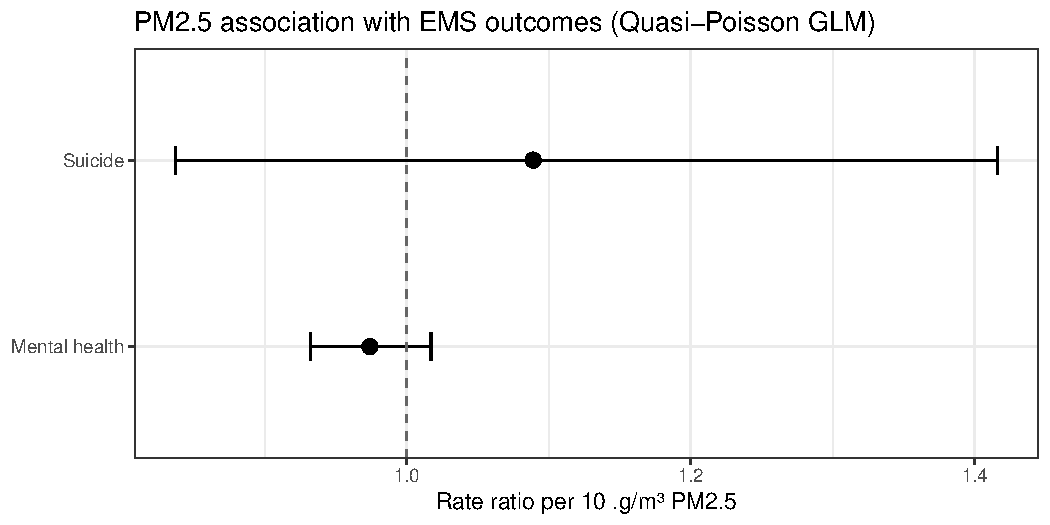
\includegraphics[keepaspectratio]{Preliminary-results_files/figure-latex/unnamed-chunk-31-1.pdf}}

\subsection{Sensitivity analysis: time trend df
(3--6)}\label{sensitivity-analysis-time-trend-df-36}

\begin{Shaded}
\begin{Highlighting}[]
\NormalTok{sens\_df }\OtherTok{\textless{}{-}} \FunctionTok{data.frame}\NormalTok{()}
\ControlFlowTok{for}\NormalTok{ (d }\ControlFlowTok{in} \DecValTok{3}\SpecialCharTok{:}\DecValTok{6}\NormalTok{) \{}
\NormalTok{  fit\_tmp }\OtherTok{\textless{}{-}} \FunctionTok{glm}\NormalTok{(mental\_health }\SpecialCharTok{\textasciitilde{}}\NormalTok{ pm25 }\SpecialCharTok{+} \FunctionTok{ns}\NormalTok{(time\_days, d) }\SpecialCharTok{+} \FunctionTok{ns}\NormalTok{(tmean, }\DecValTok{3}\NormalTok{) }\SpecialCharTok{+}
\NormalTok{                   is\_weekend }\SpecialCharTok{+}\NormalTok{ precip,}
                 \AttributeTok{family =}\NormalTok{ quasipoisson, }\AttributeTok{data =}\NormalTok{ df)}
\NormalTok{  b }\OtherTok{\textless{}{-}} \FunctionTok{coef}\NormalTok{(fit\_tmp)[}\StringTok{"pm25"}\NormalTok{]}
\NormalTok{  se }\OtherTok{\textless{}{-}} \FunctionTok{sqrt}\NormalTok{(}\FunctionTok{vcov}\NormalTok{(fit\_tmp)[}\StringTok{"pm25"}\NormalTok{, }\StringTok{"pm25"}\NormalTok{])}

\NormalTok{  sens\_df }\OtherTok{\textless{}{-}} \FunctionTok{rbind}\NormalTok{(sens\_df, }\FunctionTok{data.frame}\NormalTok{(}
    \AttributeTok{df\_time =}\NormalTok{ d,}
    \AttributeTok{outcome =} \StringTok{"Mental health"}\NormalTok{,}
    \AttributeTok{RR =} \FunctionTok{exp}\NormalTok{(b }\SpecialCharTok{*} \DecValTok{10}\NormalTok{),}
    \AttributeTok{lower =} \FunctionTok{exp}\NormalTok{((b }\SpecialCharTok{{-}} \FloatTok{1.96} \SpecialCharTok{*}\NormalTok{ se) }\SpecialCharTok{*} \DecValTok{10}\NormalTok{),}
    \AttributeTok{upper =} \FunctionTok{exp}\NormalTok{((b }\SpecialCharTok{+} \FloatTok{1.96} \SpecialCharTok{*}\NormalTok{ se) }\SpecialCharTok{*} \DecValTok{10}\NormalTok{)}
\NormalTok{  ))}

\NormalTok{  fit\_tmp2 }\OtherTok{\textless{}{-}} \FunctionTok{glm}\NormalTok{(suicide }\SpecialCharTok{\textasciitilde{}}\NormalTok{ pm25 }\SpecialCharTok{+} \FunctionTok{ns}\NormalTok{(time\_days, d) }\SpecialCharTok{+} \FunctionTok{ns}\NormalTok{(tmean, }\DecValTok{3}\NormalTok{) }\SpecialCharTok{+}
\NormalTok{                     is\_weekend }\SpecialCharTok{+}\NormalTok{ precip,}
                   \AttributeTok{family =}\NormalTok{ quasipoisson, }\AttributeTok{data =}\NormalTok{ df)}
\NormalTok{  b2 }\OtherTok{\textless{}{-}} \FunctionTok{coef}\NormalTok{(fit\_tmp2)[}\StringTok{"pm25"}\NormalTok{]}
\NormalTok{  se2 }\OtherTok{\textless{}{-}} \FunctionTok{sqrt}\NormalTok{(}\FunctionTok{vcov}\NormalTok{(fit\_tmp2)[}\StringTok{"pm25"}\NormalTok{, }\StringTok{"pm25"}\NormalTok{])}

\NormalTok{  sens\_df }\OtherTok{\textless{}{-}} \FunctionTok{rbind}\NormalTok{(sens\_df, }\FunctionTok{data.frame}\NormalTok{(}
    \AttributeTok{df\_time =}\NormalTok{ d,}
    \AttributeTok{outcome =} \StringTok{"Suicide"}\NormalTok{,}
    \AttributeTok{RR =} \FunctionTok{exp}\NormalTok{(b2 }\SpecialCharTok{*} \DecValTok{10}\NormalTok{),}
    \AttributeTok{lower =} \FunctionTok{exp}\NormalTok{((b2 }\SpecialCharTok{{-}} \FloatTok{1.96} \SpecialCharTok{*}\NormalTok{ se2) }\SpecialCharTok{*} \DecValTok{10}\NormalTok{),}
    \AttributeTok{upper =} \FunctionTok{exp}\NormalTok{((b2 }\SpecialCharTok{+} \FloatTok{1.96} \SpecialCharTok{*}\NormalTok{ se2) }\SpecialCharTok{*} \DecValTok{10}\NormalTok{)}
\NormalTok{  ))}
\NormalTok{\}}
\end{Highlighting}
\end{Shaded}

\begin{Shaded}
\begin{Highlighting}[]
\FunctionTok{ggplot}\NormalTok{(sens\_df, }\FunctionTok{aes}\NormalTok{(}\AttributeTok{x =} \FunctionTok{factor}\NormalTok{(df\_time), }\AttributeTok{y =}\NormalTok{ RR)) }\SpecialCharTok{+}
  \FunctionTok{geom\_point}\NormalTok{(}\AttributeTok{size =} \FloatTok{2.5}\NormalTok{) }\SpecialCharTok{+}
  \FunctionTok{geom\_errorbar}\NormalTok{(}\FunctionTok{aes}\NormalTok{(}\AttributeTok{ymin =}\NormalTok{ lower, }\AttributeTok{ymax =}\NormalTok{ upper), }\AttributeTok{width =} \FloatTok{0.15}\NormalTok{) }\SpecialCharTok{+}
  \FunctionTok{geom\_hline}\NormalTok{(}\AttributeTok{yintercept =} \DecValTok{1}\NormalTok{, }\AttributeTok{linetype =} \StringTok{"dashed"}\NormalTok{, }\AttributeTok{color =} \StringTok{"gray40"}\NormalTok{) }\SpecialCharTok{+}
  \FunctionTok{facet\_wrap}\NormalTok{(}\SpecialCharTok{\textasciitilde{}}\NormalTok{outcome, }\AttributeTok{scales =} \StringTok{"free\_y"}\NormalTok{) }\SpecialCharTok{+}
  \FunctionTok{labs}\NormalTok{(}\AttributeTok{x =} \StringTok{"Time trend spline df"}\NormalTok{, }\AttributeTok{y =} \StringTok{"Rate ratio per 10 μg/m³ PM2.5"}\NormalTok{,}
       \AttributeTok{title =} \StringTok{"Sensitivity of PM2.5 effect to time trend flexibility"}\NormalTok{) }\SpecialCharTok{+}
  \FunctionTok{theme\_bw}\NormalTok{(}\AttributeTok{base\_size =} \DecValTok{11}\NormalTok{)}
\end{Highlighting}
\end{Shaded}

\pandocbounded{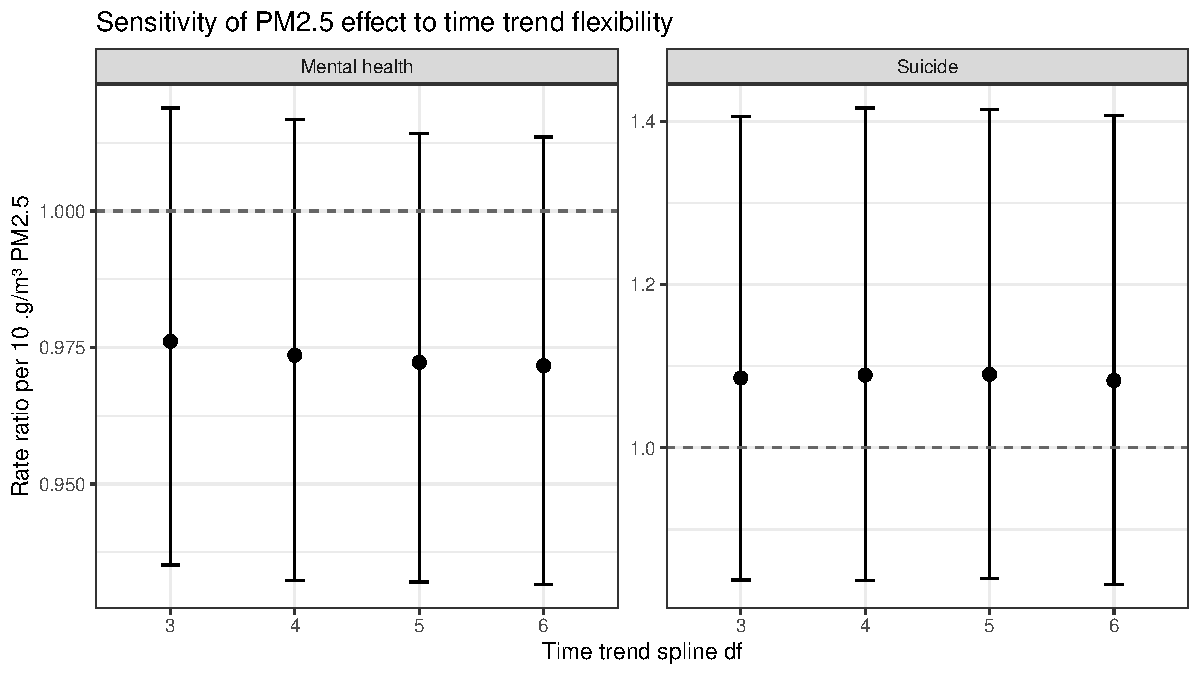
\includegraphics[keepaspectratio]{Preliminary-results_files/figure-latex/unnamed-chunk-33-1.pdf}}

\subsection{Sensitivity analysis: exclude high PM2.5
days}\label{sensitivity-analysis-exclude-high-pm2.5-days}

\begin{Shaded}
\begin{Highlighting}[]
\NormalTok{pm95\_cutoff }\OtherTok{\textless{}{-}} \FunctionTok{quantile}\NormalTok{(df}\SpecialCharTok{$}\NormalTok{pm25, }\FloatTok{0.95}\NormalTok{)}
\NormalTok{df\_trimmed }\OtherTok{\textless{}{-}}\NormalTok{ df[df}\SpecialCharTok{$}\NormalTok{pm25 }\SpecialCharTok{\textless{}=}\NormalTok{ pm95\_cutoff, ]}
\FunctionTok{cat}\NormalTok{(}\StringTok{"Excluded"}\NormalTok{, }\FunctionTok{nrow}\NormalTok{(df) }\SpecialCharTok{{-}} \FunctionTok{nrow}\NormalTok{(df\_trimmed), }\StringTok{"days with PM2.5 \textgreater{}"}\NormalTok{,}
    \FunctionTok{round}\NormalTok{(pm95\_cutoff, }\DecValTok{1}\NormalTok{), }\StringTok{"μg/m³}\SpecialCharTok{\textbackslash{}n}\StringTok{"}\NormalTok{)}
\end{Highlighting}
\end{Shaded}

\begin{verbatim}
## Excluded 7 days with PM2.5 > 12.9 μg/m³
\end{verbatim}

\begin{Shaded}
\begin{Highlighting}[]
\NormalTok{fit\_trim\_mh }\OtherTok{\textless{}{-}} \FunctionTok{glm}\NormalTok{(mental\_health }\SpecialCharTok{\textasciitilde{}}\NormalTok{ pm25 }\SpecialCharTok{+} \FunctionTok{ns}\NormalTok{(time\_days, }\DecValTok{4}\NormalTok{) }\SpecialCharTok{+} \FunctionTok{ns}\NormalTok{(tmean, }\DecValTok{3}\NormalTok{) }\SpecialCharTok{+}
\NormalTok{                      is\_weekend }\SpecialCharTok{+}\NormalTok{ precip,}
                    \AttributeTok{family =}\NormalTok{ quasipoisson, }\AttributeTok{data =}\NormalTok{ df\_trimmed)}
\NormalTok{fit\_trim\_sui }\OtherTok{\textless{}{-}} \FunctionTok{glm}\NormalTok{(suicide }\SpecialCharTok{\textasciitilde{}}\NormalTok{ pm25 }\SpecialCharTok{+} \FunctionTok{ns}\NormalTok{(time\_days, }\DecValTok{4}\NormalTok{) }\SpecialCharTok{+} \FunctionTok{ns}\NormalTok{(tmean, }\DecValTok{3}\NormalTok{) }\SpecialCharTok{+}
\NormalTok{                       is\_weekend }\SpecialCharTok{+}\NormalTok{ precip,}
                     \AttributeTok{family =}\NormalTok{ quasipoisson, }\AttributeTok{data =}\NormalTok{ df\_trimmed)}

\NormalTok{rr\_trim }\OtherTok{\textless{}{-}} \FunctionTok{rbind}\NormalTok{(}
  \FunctionTok{extract\_rr}\NormalTok{(fit\_trim\_mh, }\StringTok{"Mental health (trimmed)"}\NormalTok{),}
  \FunctionTok{extract\_rr}\NormalTok{(fit\_trim\_sui, }\StringTok{"Suicide (trimmed)"}\NormalTok{)}
\NormalTok{)}
\NormalTok{rr\_trim}\SpecialCharTok{$}\NormalTok{RR }\OtherTok{\textless{}{-}} \FunctionTok{round}\NormalTok{(rr\_trim}\SpecialCharTok{$}\NormalTok{RR, }\DecValTok{3}\NormalTok{)}
\NormalTok{rr\_trim}\SpecialCharTok{$}\NormalTok{lower }\OtherTok{\textless{}{-}} \FunctionTok{round}\NormalTok{(rr\_trim}\SpecialCharTok{$}\NormalTok{lower, }\DecValTok{3}\NormalTok{)}
\NormalTok{rr\_trim}\SpecialCharTok{$}\NormalTok{upper }\OtherTok{\textless{}{-}} \FunctionTok{round}\NormalTok{(rr\_trim}\SpecialCharTok{$}\NormalTok{upper, }\DecValTok{3}\NormalTok{)}
\NormalTok{rr\_trim}\SpecialCharTok{$}\NormalTok{p }\OtherTok{\textless{}{-}} \FunctionTok{round}\NormalTok{(rr\_trim}\SpecialCharTok{$}\NormalTok{p, }\DecValTok{3}\NormalTok{)}

\FunctionTok{rbind}\NormalTok{(rr\_table, rr\_trim)}
\end{Highlighting}
\end{Shaded}

\begin{verbatim}
##                        outcome    RR lower upper     p
## pm25             Mental health 0.974 0.932 1.017 0.228
## pm251                  Suicide 1.089 0.837 1.416 0.526
## pm252  Mental health (trimmed) 1.015 0.956 1.077 0.629
## pm2511       Suicide (trimmed) 1.023 0.699 1.498 0.908
\end{verbatim}

\subsection{Residual diagnostics}\label{residual-diagnostics}

\begin{Shaded}
\begin{Highlighting}[]
\FunctionTok{par}\NormalTok{(}\AttributeTok{mfrow =} \FunctionTok{c}\NormalTok{(}\DecValTok{1}\NormalTok{, }\DecValTok{2}\NormalTok{))}
\FunctionTok{plot}\NormalTok{(}\FunctionTok{fitted}\NormalTok{(fit\_qp\_mh), }\FunctionTok{residuals}\NormalTok{(fit\_qp\_mh, }\AttributeTok{type =} \StringTok{"deviance"}\NormalTok{),}
     \AttributeTok{xlab =} \StringTok{"Fitted"}\NormalTok{, }\AttributeTok{ylab =} \StringTok{"Deviance residuals"}\NormalTok{,}
     \AttributeTok{main =} \StringTok{"Mental health: residuals vs fitted"}\NormalTok{, }\AttributeTok{pch =} \DecValTok{16}\NormalTok{, }\AttributeTok{cex =} \FloatTok{0.7}\NormalTok{)}
\FunctionTok{abline}\NormalTok{(}\AttributeTok{h =} \DecValTok{0}\NormalTok{, }\AttributeTok{lty =} \DecValTok{2}\NormalTok{)}

\FunctionTok{plot}\NormalTok{(df}\SpecialCharTok{$}\NormalTok{date, }\FunctionTok{residuals}\NormalTok{(fit\_qp\_mh, }\AttributeTok{type =} \StringTok{"deviance"}\NormalTok{),}
     \AttributeTok{xlab =} \StringTok{"Date"}\NormalTok{, }\AttributeTok{ylab =} \StringTok{"Deviance residuals"}\NormalTok{,}
     \AttributeTok{main =} \StringTok{"Mental health: residuals over time"}\NormalTok{, }\AttributeTok{pch =} \DecValTok{16}\NormalTok{, }\AttributeTok{cex =} \FloatTok{0.7}\NormalTok{)}
\FunctionTok{abline}\NormalTok{(}\AttributeTok{h =} \DecValTok{0}\NormalTok{, }\AttributeTok{lty =} \DecValTok{2}\NormalTok{)}
\end{Highlighting}
\end{Shaded}

\pandocbounded{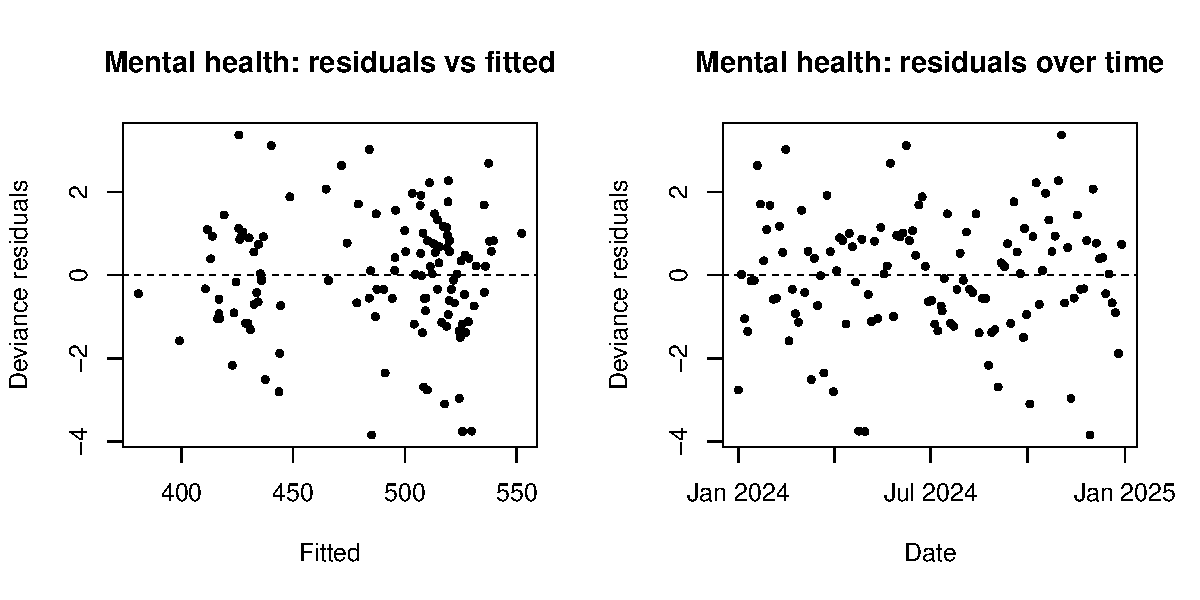
\includegraphics[keepaspectratio]{Preliminary-results_files/figure-latex/unnamed-chunk-35-1.pdf}}

\begin{Shaded}
\begin{Highlighting}[]
\FunctionTok{pacf}\NormalTok{(}\FunctionTok{residuals}\NormalTok{(fit\_qp\_mh, }\AttributeTok{type =} \StringTok{"deviance"}\NormalTok{),}
     \AttributeTok{main =} \StringTok{"PACF of deviance residuals (mental health)"}\NormalTok{)}
\end{Highlighting}
\end{Shaded}

\pandocbounded{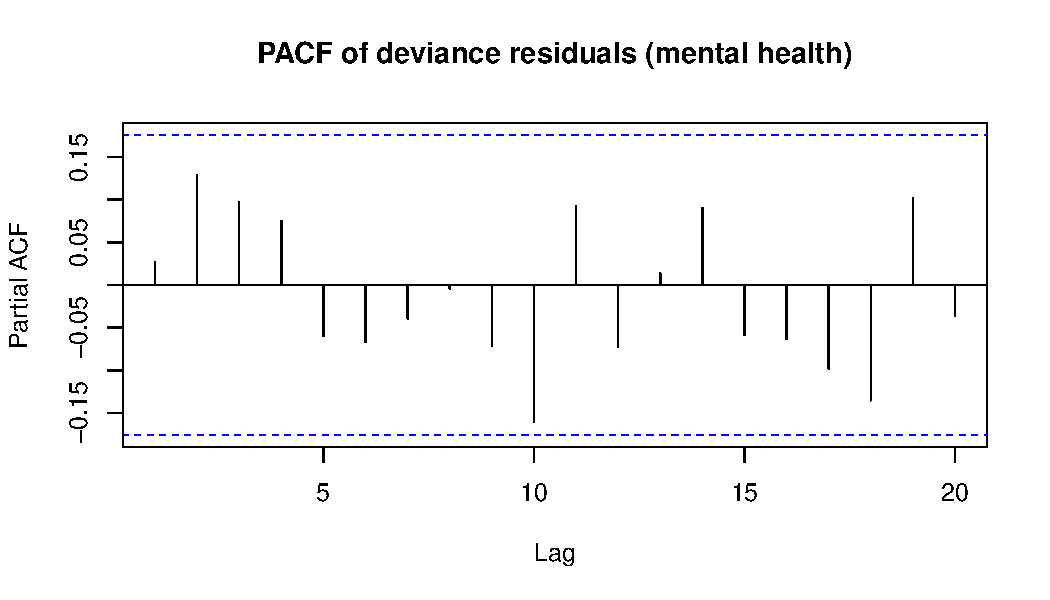
\includegraphics[keepaspectratio]{Preliminary-results_files/figure-latex/unnamed-chunk-36-1.pdf}}

\begin{Shaded}
\begin{Highlighting}[]
\FunctionTok{par}\NormalTok{(}\AttributeTok{mfrow =} \FunctionTok{c}\NormalTok{(}\DecValTok{1}\NormalTok{, }\DecValTok{2}\NormalTok{))}
\FunctionTok{plot}\NormalTok{(}\FunctionTok{fitted}\NormalTok{(fit\_qp\_sui), }\FunctionTok{residuals}\NormalTok{(fit\_qp\_sui, }\AttributeTok{type =} \StringTok{"deviance"}\NormalTok{),}
     \AttributeTok{xlab =} \StringTok{"Fitted"}\NormalTok{, }\AttributeTok{ylab =} \StringTok{"Deviance residuals"}\NormalTok{,}
     \AttributeTok{main =} \StringTok{"Suicide: residuals vs fitted"}\NormalTok{, }\AttributeTok{pch =} \DecValTok{16}\NormalTok{, }\AttributeTok{cex =} \FloatTok{0.7}\NormalTok{)}
\FunctionTok{abline}\NormalTok{(}\AttributeTok{h =} \DecValTok{0}\NormalTok{, }\AttributeTok{lty =} \DecValTok{2}\NormalTok{)}

\FunctionTok{plot}\NormalTok{(df}\SpecialCharTok{$}\NormalTok{date, }\FunctionTok{residuals}\NormalTok{(fit\_qp\_sui, }\AttributeTok{type =} \StringTok{"deviance"}\NormalTok{),}
     \AttributeTok{xlab =} \StringTok{"Date"}\NormalTok{, }\AttributeTok{ylab =} \StringTok{"Deviance residuals"}\NormalTok{,}
     \AttributeTok{main =} \StringTok{"Suicide: residuals over time"}\NormalTok{, }\AttributeTok{pch =} \DecValTok{16}\NormalTok{, }\AttributeTok{cex =} \FloatTok{0.7}\NormalTok{)}
\FunctionTok{abline}\NormalTok{(}\AttributeTok{h =} \DecValTok{0}\NormalTok{, }\AttributeTok{lty =} \DecValTok{2}\NormalTok{)}
\end{Highlighting}
\end{Shaded}

\pandocbounded{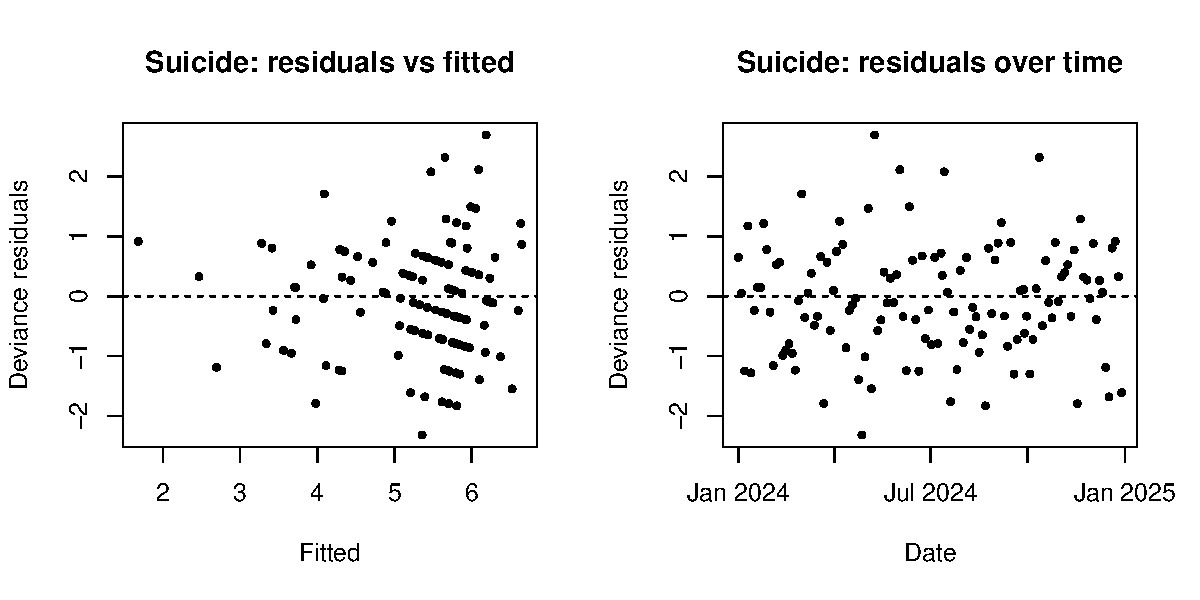
\includegraphics[keepaspectratio]{Preliminary-results_files/figure-latex/unnamed-chunk-37-1.pdf}}

\subsection{Predicted vs observed}\label{predicted-vs-observed}

\begin{Shaded}
\begin{Highlighting}[]
\NormalTok{df}\SpecialCharTok{$}\NormalTok{pred\_mh }\OtherTok{\textless{}{-}} \FunctionTok{fitted}\NormalTok{(fit\_qp\_mh)}

\FunctionTok{ggplot}\NormalTok{(df, }\FunctionTok{aes}\NormalTok{(}\AttributeTok{x =}\NormalTok{ date)) }\SpecialCharTok{+}
  \FunctionTok{geom\_point}\NormalTok{(}\FunctionTok{aes}\NormalTok{(}\AttributeTok{y =}\NormalTok{ mental\_health), }\AttributeTok{alpha =} \FloatTok{0.4}\NormalTok{, }\AttributeTok{size =} \FloatTok{1.2}\NormalTok{, }\AttributeTok{color =} \StringTok{"gray40"}\NormalTok{) }\SpecialCharTok{+}
  \FunctionTok{geom\_line}\NormalTok{(}\FunctionTok{aes}\NormalTok{(}\AttributeTok{y =}\NormalTok{ pred\_mh), }\AttributeTok{color =} \StringTok{"\#E15759"}\NormalTok{, }\AttributeTok{linewidth =} \FloatTok{0.8}\NormalTok{) }\SpecialCharTok{+}
  \FunctionTok{labs}\NormalTok{(}\AttributeTok{x =} \StringTok{"Date"}\NormalTok{, }\AttributeTok{y =} \StringTok{"Daily count"}\NormalTok{,}
       \AttributeTok{title =} \StringTok{"Mental health calls: observed vs quasi{-}Poisson fitted values"}\NormalTok{) }\SpecialCharTok{+}
  \FunctionTok{theme\_bw}\NormalTok{(}\AttributeTok{base\_size =} \DecValTok{11}\NormalTok{)}
\end{Highlighting}
\end{Shaded}

\pandocbounded{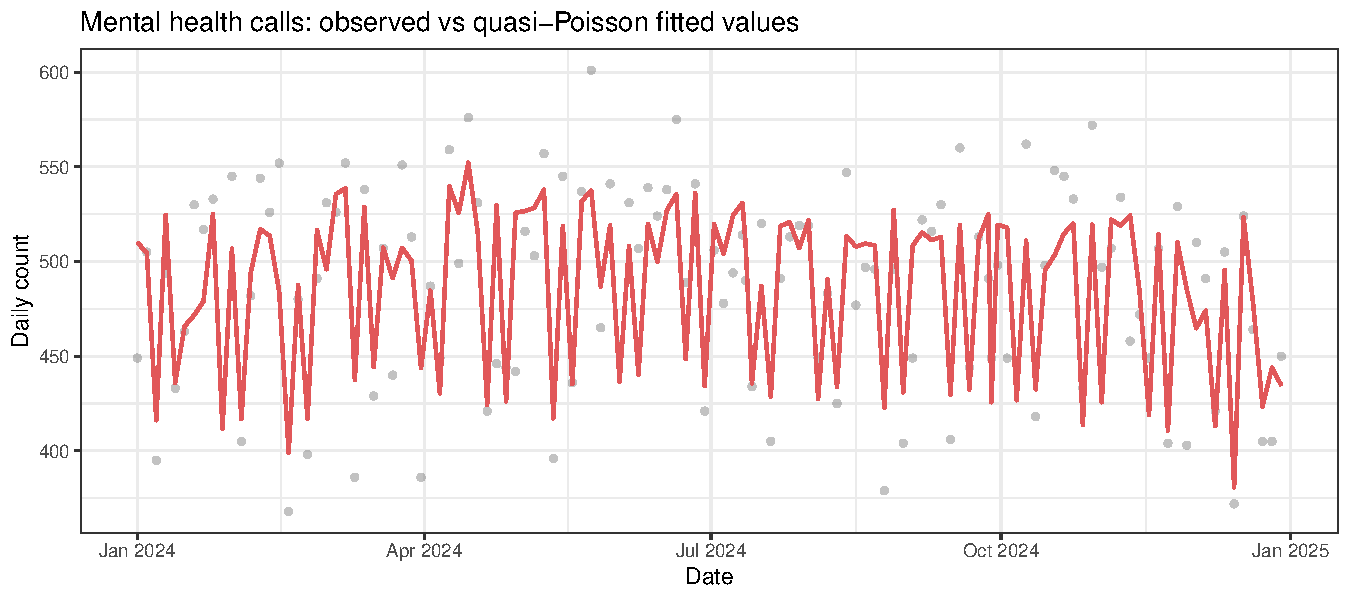
\includegraphics[keepaspectratio]{Preliminary-results_files/figure-latex/unnamed-chunk-38-1.pdf}}

\subsection{Results section outline (Quasi-Poisson
GLM)}\label{results-section-outline-quasi-poisson-glm}

The quasi-Poisson GLM estimated a rate ratio of 0.974 (95\% CI:
0.932--1.017) per 10 μg/m³ increase in same-day PM2.5 for mental health
EMS calls, after adjusting for seasonal trend, temperature, weekend, and
precipitation (p = 0.228). For suicide-related calls, the estimated rate
ratio was 1.089 (95\% CI: 0.837--1.416, p = 0.526). Neither association
was statistically significant.

Key points for the results write-up:

\begin{itemize}
\tightlist
\item
  The dispersion parameter for mental health was 2.24, confirming
  overdispersion relative to standard Poisson. For suicide calls the
  dispersion was 0.95, close to 1.
\item
  The PM2.5 coefficient was not statistically significant for either
  outcome.
\item
  Weekend indicator was a strong predictor for mental health calls
  (lower on weekends, p \textless{} 0.001), consistent with the EDA.
\item
  Sensitivity analysis: the PM2.5 rate ratio for mental health was
  stable across time trend df = 3--6 (ranging from 0.972 to 0.976).
  However, excluding high-PM2.5 days (\textgreater95th percentile)
  shifted the estimate from 0.974 to 1.015, suggesting the slight
  negative association in the main model may be driven by a few
  high-exposure days.
\item
  Residual diagnostics: check PACF plot for any remaining temporal
  autocorrelation after the time spline adjustment.
\end{itemize}

Case-crossover--Teresa Sha

\begin{Shaded}
\begin{Highlighting}[]
\FunctionTok{library}\NormalTok{(ggplot2)}
\FunctionTok{library}\NormalTok{(dplyr)}
\FunctionTok{library}\NormalTok{(lubridate)}
\FunctionTok{library}\NormalTok{(broom)}
\end{Highlighting}
\end{Shaded}

\begin{Shaded}
\begin{Highlighting}[]
\DocumentationTok{\#\#\#\#\#\#\#\#\#\#\#\#\#\#\#\#\#\#\#\#\#\#\#\#\#\#\#\#\#\#\#\#\#\#\#\#\#\#\#\#\#\#\#\#\#\#\#\#\#\#\#\#\#\#\#\#\#\#\#\#}
\DocumentationTok{\#\# case\_crossover\_sensitivity.R}
\DocumentationTok{\#\# Sensitivity analysis:}
\DocumentationTok{\#\# time{-}stratified case{-}crossover using conditional Poisson}
\DocumentationTok{\#\#\#\#\#\#\#\#\#\#\#\#\#\#\#\#\#\#\#\#\#\#\#\#\#\#\#\#\#\#\#\#\#\#\#\#\#\#\#\#\#\#\#\#\#\#\#\#\#\#\#\#\#\#\#\#\#\#\#\#}

\DocumentationTok{\#\# {-}{-}{-}{-}{-}{-}{-}{-}{-}{-}{-}{-}{-}{-}{-}{-}{-}{-}{-}{-}{-}{-}{-}{-}{-}{-}{-}}
\DocumentationTok{\#\# 0. packages}
\DocumentationTok{\#\# {-}{-}{-}{-}{-}{-}{-}{-}{-}{-}{-}{-}{-}{-}{-}{-}{-}{-}{-}{-}{-}{-}{-}{-}{-}{-}{-}}
\NormalTok{packages }\OtherTok{\textless{}{-}} \FunctionTok{c}\NormalTok{(}\StringTok{"dplyr"}\NormalTok{, }\StringTok{"lubridate"}\NormalTok{, }\StringTok{"splines"}\NormalTok{, }\StringTok{"gnm"}\NormalTok{, }\StringTok{"broom"}\NormalTok{)}

\NormalTok{to\_install }\OtherTok{\textless{}{-}}\NormalTok{ packages[}\SpecialCharTok{!}\NormalTok{packages }\SpecialCharTok{\%in\%} \FunctionTok{installed.packages}\NormalTok{()[, }\StringTok{"Package"}\NormalTok{]]}
\ControlFlowTok{if}\NormalTok{ (}\FunctionTok{length}\NormalTok{(to\_install) }\SpecialCharTok{\textgreater{}} \DecValTok{0}\NormalTok{) }\FunctionTok{install.packages}\NormalTok{(to\_install)}

\FunctionTok{library}\NormalTok{(dplyr)}
\FunctionTok{library}\NormalTok{(lubridate)}
\FunctionTok{library}\NormalTok{(splines)}
\FunctionTok{library}\NormalTok{(gnm)}
\FunctionTok{library}\NormalTok{(broom)}
\end{Highlighting}
\end{Shaded}

\begin{Shaded}
\begin{Highlighting}[]
\DocumentationTok{\#\# {-}{-}{-}{-}{-}{-}{-}{-}{-}{-}{-}{-}{-}{-}{-}{-}{-}{-}{-}{-}{-}{-}{-}{-}{-}{-}{-}}
\DocumentationTok{\#\# 1. read data}
\DocumentationTok{\#\# {-}{-}{-}{-}{-}{-}{-}{-}{-}{-}{-}{-}{-}{-}{-}{-}{-}{-}{-}{-}{-}{-}{-}{-}{-}{-}{-}}
\DocumentationTok{\#\# Choose ONE path that matches your own folder structure.}

\DocumentationTok{\#\# Option A: if your script is inside the project folder}
\DocumentationTok{\#\# and analysis\_2024.csv is in data/}
\NormalTok{file\_path }\OtherTok{\textless{}{-}} \StringTok{"data/analysis\_2024.csv"}

\DocumentationTok{\#\# Option B: if analysis\_2024.csv is in the same folder as this script}
\DocumentationTok{\#\# file\_path \textless{}{-} "analysis\_2024.csv"}

\DocumentationTok{\#\# Option C: if you want to use full local path on your computer}
\DocumentationTok{\#\# file\_path \textless{}{-} "/Users/yourname/Desktop/aa\_project/data/analysis\_2024.csv"}

\NormalTok{df }\OtherTok{\textless{}{-}} \FunctionTok{read.csv}\NormalTok{(file\_path)}
\end{Highlighting}
\end{Shaded}

\begin{Shaded}
\begin{Highlighting}[]
\DocumentationTok{\#\# {-}{-}{-}{-}{-}{-}{-}{-}{-}{-}{-}{-}{-}{-}{-}{-}{-}{-}{-}{-}{-}{-}{-}{-}{-}{-}{-}}
\DocumentationTok{\#\# 2. basic cleaning}
\DocumentationTok{\#\# {-}{-}{-}{-}{-}{-}{-}{-}{-}{-}{-}{-}{-}{-}{-}{-}{-}{-}{-}{-}{-}{-}{-}{-}{-}{-}{-}}
\NormalTok{df }\OtherTok{\textless{}{-}}\NormalTok{ df }\SpecialCharTok{\%\textgreater{}\%}
  \FunctionTok{mutate}\NormalTok{(}
    \AttributeTok{date =} \FunctionTok{as.Date}\NormalTok{(date),}
    \AttributeTok{year =} \FunctionTok{year}\NormalTok{(date),}
    \AttributeTok{month\_num =} \FunctionTok{month}\NormalTok{(date),}
    \AttributeTok{dow\_num =} \FunctionTok{wday}\NormalTok{(date, }\AttributeTok{week\_start =} \DecValTok{1}\NormalTok{),  }\CommentTok{\# Monday = 1}
    \AttributeTok{dow\_name =} \FunctionTok{factor}\NormalTok{(}
\NormalTok{      dow\_num,}
      \AttributeTok{levels =} \DecValTok{1}\SpecialCharTok{:}\DecValTok{7}\NormalTok{,}
      \AttributeTok{labels =} \FunctionTok{c}\NormalTok{(}\StringTok{"Mon"}\NormalTok{, }\StringTok{"Tue"}\NormalTok{, }\StringTok{"Wed"}\NormalTok{, }\StringTok{"Thu"}\NormalTok{, }\StringTok{"Fri"}\NormalTok{, }\StringTok{"Sat"}\NormalTok{, }\StringTok{"Sun"}\NormalTok{)}
\NormalTok{    )}
\NormalTok{  ) }\SpecialCharTok{\%\textgreater{}\%}
  \FunctionTok{arrange}\NormalTok{(date)}

\DocumentationTok{\#\# Quick check}
\FunctionTok{cat}\NormalTok{(}\StringTok{"Rows:"}\NormalTok{, }\FunctionTok{nrow}\NormalTok{(df), }\StringTok{"}\SpecialCharTok{\textbackslash{}n}\StringTok{"}\NormalTok{)}
\end{Highlighting}
\end{Shaded}

\begin{verbatim}
## Rows: 124
\end{verbatim}

\begin{Shaded}
\begin{Highlighting}[]
\FunctionTok{cat}\NormalTok{(}\StringTok{"Date range:"}\NormalTok{, }\FunctionTok{as.character}\NormalTok{(}\FunctionTok{min}\NormalTok{(df}\SpecialCharTok{$}\NormalTok{date)), }\StringTok{"to"}\NormalTok{, }\FunctionTok{as.character}\NormalTok{(}\FunctionTok{max}\NormalTok{(df}\SpecialCharTok{$}\NormalTok{date)), }\StringTok{"}\SpecialCharTok{\textbackslash{}n}\StringTok{"}\NormalTok{)}
\end{Highlighting}
\end{Shaded}

\begin{verbatim}
## Date range: 2024-01-01 to 2024-12-29
\end{verbatim}

\begin{Shaded}
\begin{Highlighting}[]
\FunctionTok{print}\NormalTok{(}\FunctionTok{names}\NormalTok{(df))}
\end{Highlighting}
\end{Shaded}

\begin{verbatim}
##  [1] "date"          "pm25"          "mental_health" "suicide"      
##  [5] "tmax"          "tmin"          "tmean"         "precip"       
##  [9] "windspeed"     "rh_max"        "month"         "weekday"      
## [13] "is_weekend"    "heat_day"      "year"          "month_num"    
## [17] "dow_num"       "dow_name"
\end{verbatim}

\begin{Shaded}
\begin{Highlighting}[]
\DocumentationTok{\#\# {-}{-}{-}{-}{-}{-}{-}{-}{-}{-}{-}{-}{-}{-}{-}{-}{-}{-}{-}{-}{-}{-}{-}{-}{-}{-}{-}}
\DocumentationTok{\#\# 3. create case{-}crossover strata}
\DocumentationTok{\#\# {-}{-}{-}{-}{-}{-}{-}{-}{-}{-}{-}{-}{-}{-}{-}{-}{-}{-}{-}{-}{-}{-}{-}{-}{-}{-}{-}}
\DocumentationTok{\#\# Time{-}stratified control selection:}
\DocumentationTok{\#\# same year + same month + same day of week}
\DocumentationTok{\#\# This matches the usual case{-}crossover setup.}

\NormalTok{df }\OtherTok{\textless{}{-}}\NormalTok{ df }\SpecialCharTok{\%\textgreater{}\%}
  \FunctionTok{mutate}\NormalTok{(}
    \AttributeTok{stratum =} \FunctionTok{interaction}\NormalTok{(year, month\_num, dow\_name, }\AttributeTok{drop =} \ConstantTok{TRUE}\NormalTok{)}
\NormalTok{  )}

\DocumentationTok{\#\# Keep only strata with at least 2 observed days}
\DocumentationTok{\#\# because strata with only 1 row do not contribute within{-}stratum comparison}
\NormalTok{df\_cc }\OtherTok{\textless{}{-}}\NormalTok{ df }\SpecialCharTok{\%\textgreater{}\%}
  \FunctionTok{group\_by}\NormalTok{(stratum) }\SpecialCharTok{\%\textgreater{}\%}
  \FunctionTok{mutate}\NormalTok{(}\AttributeTok{n\_in\_stratum =} \FunctionTok{n}\NormalTok{()) }\SpecialCharTok{\%\textgreater{}\%}
  \FunctionTok{ungroup}\NormalTok{() }\SpecialCharTok{\%\textgreater{}\%}
  \FunctionTok{filter}\NormalTok{(n\_in\_stratum }\SpecialCharTok{\textgreater{}=} \DecValTok{2}\NormalTok{)}

\FunctionTok{cat}\NormalTok{(}\StringTok{"Rows after dropping singleton strata:"}\NormalTok{, }\FunctionTok{nrow}\NormalTok{(df\_cc), }\StringTok{"}\SpecialCharTok{\textbackslash{}n}\StringTok{"}\NormalTok{)}
\end{Highlighting}
\end{Shaded}

\begin{verbatim}
## Rows after dropping singleton strata: 79
\end{verbatim}

\begin{Shaded}
\begin{Highlighting}[]
\FunctionTok{cat}\NormalTok{(}\StringTok{"Number of strata kept:"}\NormalTok{, }\FunctionTok{n\_distinct}\NormalTok{(df\_cc}\SpecialCharTok{$}\NormalTok{stratum), }\StringTok{"}\SpecialCharTok{\textbackslash{}n}\StringTok{"}\NormalTok{)}
\end{Highlighting}
\end{Shaded}

\begin{verbatim}
## Number of strata kept: 39
\end{verbatim}

\begin{Shaded}
\begin{Highlighting}[]
\DocumentationTok{\#\# {-}{-}{-}{-}{-}{-}{-}{-}{-}{-}{-}{-}{-}{-}{-}{-}{-}{-}{-}{-}{-}{-}{-}{-}{-}{-}{-}}
\DocumentationTok{\#\# 4. create lag variables}
\DocumentationTok{\#\# {-}{-}{-}{-}{-}{-}{-}{-}{-}{-}{-}{-}{-}{-}{-}{-}{-}{-}{-}{-}{-}{-}{-}{-}{-}{-}{-}}
\DocumentationTok{\#\# Since PM2.5 is measured only on selected days,}
\DocumentationTok{\#\# these lags are based on previous observed row in the merged dataset.}
\DocumentationTok{\#\# For this sensitivity analysis, lag 0 and lag 1 are enough.}

\NormalTok{df\_cc }\OtherTok{\textless{}{-}}\NormalTok{ df\_cc }\SpecialCharTok{\%\textgreater{}\%}
  \FunctionTok{arrange}\NormalTok{(date) }\SpecialCharTok{\%\textgreater{}\%}
  \FunctionTok{mutate}\NormalTok{(}
    \AttributeTok{pm25\_lag1 =} \FunctionTok{lag}\NormalTok{(pm25, }\DecValTok{1}\NormalTok{),}
    \AttributeTok{pm25\_lag2 =} \FunctionTok{lag}\NormalTok{(pm25, }\DecValTok{2}\NormalTok{),}
    \AttributeTok{tmean\_lag1 =} \FunctionTok{lag}\NormalTok{(tmean, }\DecValTok{1}\NormalTok{),}
    \AttributeTok{rh\_max\_lag1 =} \FunctionTok{lag}\NormalTok{(rh\_max, }\DecValTok{1}\NormalTok{)}
\NormalTok{  )}

\DocumentationTok{\#\# Datasets for lag models}
\NormalTok{df\_cc\_lag1 }\OtherTok{\textless{}{-}}\NormalTok{ df\_cc }\SpecialCharTok{\%\textgreater{}\%}
  \FunctionTok{filter}\NormalTok{(}\SpecialCharTok{!}\FunctionTok{is.na}\NormalTok{(pm25\_lag1), }\SpecialCharTok{!}\FunctionTok{is.na}\NormalTok{(tmean\_lag1), }\SpecialCharTok{!}\FunctionTok{is.na}\NormalTok{(rh\_max\_lag1))}

\NormalTok{df\_cc\_lag2 }\OtherTok{\textless{}{-}}\NormalTok{ df\_cc }\SpecialCharTok{\%\textgreater{}\%}
  \FunctionTok{filter}\NormalTok{(}\SpecialCharTok{!}\FunctionTok{is.na}\NormalTok{(pm25\_lag1), }\SpecialCharTok{!}\FunctionTok{is.na}\NormalTok{(pm25\_lag2),}
         \SpecialCharTok{!}\FunctionTok{is.na}\NormalTok{(tmean\_lag1), }\SpecialCharTok{!}\FunctionTok{is.na}\NormalTok{(rh\_max\_lag1))}
\end{Highlighting}
\end{Shaded}

\begin{Shaded}
\begin{Highlighting}[]
\DocumentationTok{\#\# {-}{-}{-}{-}{-}{-}{-}{-}{-}{-}{-}{-}{-}{-}{-}{-}{-}{-}{-}{-}{-}{-}{-}{-}{-}{-}{-}}
\DocumentationTok{\#\# 5. helper function for IRR output}
\DocumentationTok{\#\# {-}{-}{-}{-}{-}{-}{-}{-}{-}{-}{-}{-}{-}{-}{-}{-}{-}{-}{-}{-}{-}{-}{-}{-}{-}{-}{-}}
\NormalTok{get\_irr }\OtherTok{\textless{}{-}} \ControlFlowTok{function}\NormalTok{(model, }\AttributeTok{exposure\_name =} \StringTok{"pm25"}\NormalTok{, }\AttributeTok{increment =} \DecValTok{1}\NormalTok{) \{}
\NormalTok{  beta }\OtherTok{\textless{}{-}} \FunctionTok{coef}\NormalTok{(model)[exposure\_name]}
\NormalTok{  se   }\OtherTok{\textless{}{-}} \FunctionTok{sqrt}\NormalTok{(}\FunctionTok{vcov}\NormalTok{(model)[exposure\_name, exposure\_name])}

\NormalTok{  est  }\OtherTok{\textless{}{-}} \FunctionTok{exp}\NormalTok{(beta }\SpecialCharTok{*}\NormalTok{ increment)}
\NormalTok{  low  }\OtherTok{\textless{}{-}} \FunctionTok{exp}\NormalTok{((beta }\SpecialCharTok{{-}} \FloatTok{1.96} \SpecialCharTok{*}\NormalTok{ se) }\SpecialCharTok{*}\NormalTok{ increment)}
\NormalTok{  high }\OtherTok{\textless{}{-}} \FunctionTok{exp}\NormalTok{((beta }\SpecialCharTok{+} \FloatTok{1.96} \SpecialCharTok{*}\NormalTok{ se) }\SpecialCharTok{*}\NormalTok{ increment)}

\NormalTok{  out }\OtherTok{\textless{}{-}} \FunctionTok{data.frame}\NormalTok{(}
    \AttributeTok{term =}\NormalTok{ exposure\_name,}
    \AttributeTok{increment =}\NormalTok{ increment,}
    \AttributeTok{IRR =}\NormalTok{ est,}
    \AttributeTok{CI\_low =}\NormalTok{ low,}
    \AttributeTok{CI\_high =}\NormalTok{ high}
\NormalTok{  )}
  \FunctionTok{return}\NormalTok{(out)}
\NormalTok{\}}
\end{Highlighting}
\end{Shaded}

\begin{Shaded}
\begin{Highlighting}[]
\DocumentationTok{\#\# {-}{-}{-}{-}{-}{-}{-}{-}{-}{-}{-}{-}{-}{-}{-}{-}{-}{-}{-}{-}{-}{-}{-}{-}{-}{-}{-}}
\DocumentationTok{\#\# 6. main conditional Poisson models}
\DocumentationTok{\#\# {-}{-}{-}{-}{-}{-}{-}{-}{-}{-}{-}{-}{-}{-}{-}{-}{-}{-}{-}{-}{-}{-}{-}{-}{-}{-}{-}}
\DocumentationTok{\#\# Outcome 1: mental\_health}
\DocumentationTok{\#\# Model 1: lag 0 only}
\NormalTok{m\_mh\_lag0 }\OtherTok{\textless{}{-}} \FunctionTok{gnm}\NormalTok{(}
\NormalTok{  mental\_health }\SpecialCharTok{\textasciitilde{}}\NormalTok{ pm25 }\SpecialCharTok{+} \FunctionTok{ns}\NormalTok{(tmean, }\AttributeTok{df =} \DecValTok{3}\NormalTok{) }\SpecialCharTok{+} \FunctionTok{ns}\NormalTok{(rh\_max, }\AttributeTok{df =} \DecValTok{3}\NormalTok{),}
  \AttributeTok{eliminate =}\NormalTok{ stratum,}
  \AttributeTok{family =} \FunctionTok{quasipoisson}\NormalTok{(}\AttributeTok{link =} \StringTok{"log"}\NormalTok{),}
  \AttributeTok{data =}\NormalTok{ df\_cc}
\NormalTok{)}
\end{Highlighting}
\end{Shaded}

\begin{Shaded}
\begin{Highlighting}[]
\DocumentationTok{\#\# Model 2: lag 0 + lag 1}
\NormalTok{m\_mh\_lag01 }\OtherTok{\textless{}{-}} \FunctionTok{gnm}\NormalTok{(}
\NormalTok{  mental\_health }\SpecialCharTok{\textasciitilde{}}\NormalTok{ pm25 }\SpecialCharTok{+}\NormalTok{ pm25\_lag1 }\SpecialCharTok{+} \FunctionTok{ns}\NormalTok{(tmean, }\AttributeTok{df =} \DecValTok{3}\NormalTok{) }\SpecialCharTok{+} \FunctionTok{ns}\NormalTok{(rh\_max, }\AttributeTok{df =} \DecValTok{3}\NormalTok{),}
  \AttributeTok{eliminate =}\NormalTok{ stratum,}
  \AttributeTok{family =} \FunctionTok{quasipoisson}\NormalTok{(}\AttributeTok{link =} \StringTok{"log"}\NormalTok{),}
  \AttributeTok{data =}\NormalTok{ df\_cc\_lag1}
\NormalTok{)}
\end{Highlighting}
\end{Shaded}

\begin{Shaded}
\begin{Highlighting}[]
\DocumentationTok{\#\# Model 3: interaction with heat\_day}
\NormalTok{m\_mh\_interaction }\OtherTok{\textless{}{-}} \FunctionTok{gnm}\NormalTok{(}
\NormalTok{  mental\_health }\SpecialCharTok{\textasciitilde{}}\NormalTok{ pm25 }\SpecialCharTok{*}\NormalTok{ heat\_day }\SpecialCharTok{+} \FunctionTok{ns}\NormalTok{(tmean, }\AttributeTok{df =} \DecValTok{3}\NormalTok{) }\SpecialCharTok{+} \FunctionTok{ns}\NormalTok{(rh\_max, }\AttributeTok{df =} \DecValTok{3}\NormalTok{),}
  \AttributeTok{eliminate =}\NormalTok{ stratum,}
  \AttributeTok{family =} \FunctionTok{quasipoisson}\NormalTok{(}\AttributeTok{link =} \StringTok{"log"}\NormalTok{),}
  \AttributeTok{data =}\NormalTok{ df\_cc}
\NormalTok{)}
\end{Highlighting}
\end{Shaded}

\begin{Shaded}
\begin{Highlighting}[]
\DocumentationTok{\#\# Outcome 2: suicide}
\DocumentationTok{\#\# Model 4: lag 0 only}
\NormalTok{m\_su\_lag0 }\OtherTok{\textless{}{-}} \FunctionTok{gnm}\NormalTok{(}
\NormalTok{  suicide }\SpecialCharTok{\textasciitilde{}}\NormalTok{ pm25 }\SpecialCharTok{+} \FunctionTok{ns}\NormalTok{(tmean, }\AttributeTok{df =} \DecValTok{3}\NormalTok{) }\SpecialCharTok{+} \FunctionTok{ns}\NormalTok{(rh\_max, }\AttributeTok{df =} \DecValTok{3}\NormalTok{),}
  \AttributeTok{eliminate =}\NormalTok{ stratum,}
  \AttributeTok{family =} \FunctionTok{quasipoisson}\NormalTok{(}\AttributeTok{link =} \StringTok{"log"}\NormalTok{),}
  \AttributeTok{data =}\NormalTok{ df\_cc}
\NormalTok{)}
\end{Highlighting}
\end{Shaded}

\begin{Shaded}
\begin{Highlighting}[]
\DocumentationTok{\#\# Model 5: lag 0 + lag 1}
\NormalTok{m\_su\_lag01 }\OtherTok{\textless{}{-}} \FunctionTok{gnm}\NormalTok{(}
\NormalTok{  suicide }\SpecialCharTok{\textasciitilde{}}\NormalTok{ pm25 }\SpecialCharTok{+}\NormalTok{ pm25\_lag1 }\SpecialCharTok{+} \FunctionTok{ns}\NormalTok{(tmean, }\AttributeTok{df =} \DecValTok{3}\NormalTok{) }\SpecialCharTok{+} \FunctionTok{ns}\NormalTok{(rh\_max, }\AttributeTok{df =} \DecValTok{3}\NormalTok{),}
  \AttributeTok{eliminate =}\NormalTok{ stratum,}
  \AttributeTok{family =} \FunctionTok{quasipoisson}\NormalTok{(}\AttributeTok{link =} \StringTok{"log"}\NormalTok{),}
  \AttributeTok{data =}\NormalTok{ df\_cc\_lag1}
\NormalTok{)}
\end{Highlighting}
\end{Shaded}

\begin{Shaded}
\begin{Highlighting}[]
\DocumentationTok{\#\# {-}{-}{-}{-}{-}{-}{-}{-}{-}{-}{-}{-}{-}{-}{-}{-}{-}{-}{-}{-}{-}{-}{-}{-}{-}{-}{-}}
\DocumentationTok{\#\# 7. optional: two{-}pollutant{-}style lag sensitivity}
\DocumentationTok{\#\# {-}{-}{-}{-}{-}{-}{-}{-}{-}{-}{-}{-}{-}{-}{-}{-}{-}{-}{-}{-}{-}{-}{-}{-}{-}{-}{-}}
\DocumentationTok{\#\# This one is optional. Use only if you want one extra robustness check.}
\NormalTok{m\_mh\_lag012 }\OtherTok{\textless{}{-}} \FunctionTok{gnm}\NormalTok{(}
\NormalTok{  mental\_health }\SpecialCharTok{\textasciitilde{}}\NormalTok{ pm25 }\SpecialCharTok{+}\NormalTok{ pm25\_lag1 }\SpecialCharTok{+}\NormalTok{ pm25\_lag2 }\SpecialCharTok{+}
    \FunctionTok{ns}\NormalTok{(tmean, }\AttributeTok{df =} \DecValTok{3}\NormalTok{) }\SpecialCharTok{+} \FunctionTok{ns}\NormalTok{(rh\_max, }\AttributeTok{df =} \DecValTok{3}\NormalTok{),}
  \AttributeTok{eliminate =}\NormalTok{ stratum,}
  \AttributeTok{family =} \FunctionTok{quasipoisson}\NormalTok{(}\AttributeTok{link =} \StringTok{"log"}\NormalTok{),}
  \AttributeTok{data =}\NormalTok{ df\_cc\_lag2}
\NormalTok{)}
\end{Highlighting}
\end{Shaded}

\begin{Shaded}
\begin{Highlighting}[]
\DocumentationTok{\#\# {-}{-}{-}{-}{-}{-}{-}{-}{-}{-}{-}{-}{-}{-}{-}{-}{-}{-}{-}{-}{-}{-}{-}{-}{-}{-}{-}}
\DocumentationTok{\#\# 8. model summaries}
\DocumentationTok{\#\# {-}{-}{-}{-}{-}{-}{-}{-}{-}{-}{-}{-}{-}{-}{-}{-}{-}{-}{-}{-}{-}{-}{-}{-}{-}{-}{-}}
\FunctionTok{cat}\NormalTok{(}\StringTok{"}\SpecialCharTok{\textbackslash{}n}\StringTok{==============================}\SpecialCharTok{\textbackslash{}n}\StringTok{"}\NormalTok{)}
\end{Highlighting}
\end{Shaded}

\begin{verbatim}
## 
## ==============================
\end{verbatim}

\begin{Shaded}
\begin{Highlighting}[]
\FunctionTok{cat}\NormalTok{(}\StringTok{"Mental health model: lag 0}\SpecialCharTok{\textbackslash{}n}\StringTok{"}\NormalTok{)}
\end{Highlighting}
\end{Shaded}

\begin{verbatim}
## Mental health model: lag 0
\end{verbatim}

\begin{Shaded}
\begin{Highlighting}[]
\FunctionTok{cat}\NormalTok{(}\StringTok{"==============================}\SpecialCharTok{\textbackslash{}n}\StringTok{"}\NormalTok{)}
\end{Highlighting}
\end{Shaded}

\begin{verbatim}
## ==============================
\end{verbatim}

\begin{Shaded}
\begin{Highlighting}[]
\FunctionTok{print}\NormalTok{(}\FunctionTok{summary}\NormalTok{(m\_mh\_lag0))}
\end{Highlighting}
\end{Shaded}

\begin{verbatim}
## 
## Call:
## gnm(formula = mental_health ~ pm25 + ns(tmean, df = 3) + ns(rh_max, 
##     df = 3), eliminate = stratum, family = quasipoisson(link = "log"), 
##     data = df_cc)
## 
## Deviance Residuals: 
##     Min       1Q   Median       3Q      Max  
## -2.4181  -0.7097  -0.0283   0.6894   2.3079  
## 
## Coefficients of interest:
##                      Estimate Std. Error t value Pr(>|t|)  
## pm25                -0.001336   0.004401  -0.304   0.7634  
## ns(tmean, df = 3)1   0.228609   0.113062   2.022   0.0513 .
## ns(tmean, df = 3)2   0.607092   0.236943   2.562   0.0152 *
## ns(tmean, df = 3)3   0.235283   0.125015   1.882   0.0687 .
## ns(rh_max, df = 3)1 -0.052486   0.049808  -1.054   0.2996  
## ns(rh_max, df = 3)2 -0.037057   0.164707  -0.225   0.8234  
## ns(rh_max, df = 3)3 -0.059026   0.043303  -1.363   0.1821  
## ---
## Signif. codes:  0 '***' 0.001 '**' 0.01 '*' 0.05 '.' 0.1 ' ' 1
## 
## (Dispersion parameter for quasipoisson family taken to be 3.018922)
## 
## Residual deviance: 99.724 on 33 degrees of freedom
## AIC: NA
## 
## Number of iterations: 2
\end{verbatim}

\begin{Shaded}
\begin{Highlighting}[]
\FunctionTok{cat}\NormalTok{(}\StringTok{"}\SpecialCharTok{\textbackslash{}n}\StringTok{==============================}\SpecialCharTok{\textbackslash{}n}\StringTok{"}\NormalTok{)}
\end{Highlighting}
\end{Shaded}

\begin{verbatim}
## 
## ==============================
\end{verbatim}

\begin{Shaded}
\begin{Highlighting}[]
\FunctionTok{cat}\NormalTok{(}\StringTok{"Mental health model: lag 0 + lag 1}\SpecialCharTok{\textbackslash{}n}\StringTok{"}\NormalTok{)}
\end{Highlighting}
\end{Shaded}

\begin{verbatim}
## Mental health model: lag 0 + lag 1
\end{verbatim}

\begin{Shaded}
\begin{Highlighting}[]
\FunctionTok{cat}\NormalTok{(}\StringTok{"==============================}\SpecialCharTok{\textbackslash{}n}\StringTok{"}\NormalTok{)}
\end{Highlighting}
\end{Shaded}

\begin{verbatim}
## ==============================
\end{verbatim}

\begin{Shaded}
\begin{Highlighting}[]
\FunctionTok{print}\NormalTok{(}\FunctionTok{summary}\NormalTok{(m\_mh\_lag01))}
\end{Highlighting}
\end{Shaded}

\begin{verbatim}
## 
## Call:
## gnm(formula = mental_health ~ pm25 + pm25_lag1 + ns(tmean, df = 3) + 
##     ns(rh_max, df = 3), eliminate = stratum, family = quasipoisson(link = "log"), 
##     data = df_cc_lag1)
## 
## Deviance Residuals: 
##       Min         1Q     Median         3Q        Max  
## -2.356804  -0.621264  -0.001059   0.593190   2.245231  
## 
## Coefficients of interest:
##                       Estimate Std. Error t value Pr(>|t|)   
## pm25                -0.0009464  0.0044853  -0.211  0.83426   
## pm25_lag1            0.0011654  0.0037695   0.309  0.75927   
## ns(tmean, df = 3)1   0.2596876  0.1142668   2.273  0.03013 * 
## ns(tmean, df = 3)2   0.7190841  0.2441077   2.946  0.00607 **
## ns(tmean, df = 3)3   0.2343291  0.1281730   1.828  0.07715 . 
## ns(rh_max, df = 3)1 -0.0363880  0.0496487  -0.733  0.46912   
## ns(rh_max, df = 3)2 -0.0782739  0.1638991  -0.478  0.63630   
## ns(rh_max, df = 3)3 -0.0566455  0.0428757  -1.321  0.19612   
## ---
## Signif. codes:  0 '***' 0.001 '**' 0.01 '*' 0.05 '.' 0.1 ' ' 1
## 
## (Dispersion parameter for quasipoisson family taken to be 2.896589)
## 
## Residual deviance: 89.881 on 31 degrees of freedom
## AIC: NA
## 
## Number of iterations: 2
\end{verbatim}

\begin{Shaded}
\begin{Highlighting}[]
\FunctionTok{cat}\NormalTok{(}\StringTok{"}\SpecialCharTok{\textbackslash{}n}\StringTok{==============================}\SpecialCharTok{\textbackslash{}n}\StringTok{"}\NormalTok{)}
\end{Highlighting}
\end{Shaded}

\begin{verbatim}
## 
## ==============================
\end{verbatim}

\begin{Shaded}
\begin{Highlighting}[]
\FunctionTok{cat}\NormalTok{(}\StringTok{"Mental health model: PM2.5 * heat\_day}\SpecialCharTok{\textbackslash{}n}\StringTok{"}\NormalTok{)}
\end{Highlighting}
\end{Shaded}

\begin{verbatim}
## Mental health model: PM2.5 * heat_day
\end{verbatim}

\begin{Shaded}
\begin{Highlighting}[]
\FunctionTok{cat}\NormalTok{(}\StringTok{"==============================}\SpecialCharTok{\textbackslash{}n}\StringTok{"}\NormalTok{)}
\end{Highlighting}
\end{Shaded}

\begin{verbatim}
## ==============================
\end{verbatim}

\begin{Shaded}
\begin{Highlighting}[]
\FunctionTok{print}\NormalTok{(}\FunctionTok{summary}\NormalTok{(m\_mh\_interaction))}
\end{Highlighting}
\end{Shaded}

\begin{verbatim}
## 
## Call:
## gnm(formula = mental_health ~ pm25 * heat_day + ns(tmean, df = 3) + 
##     ns(rh_max, df = 3), eliminate = stratum, family = quasipoisson(link = "log"), 
##     data = df_cc)
## 
## Deviance Residuals: 
##      Min        1Q    Median        3Q       Max  
## -2.40868  -0.71331   0.03417   0.68187   2.29825  
## 
## Coefficients of interest:
##                      Estimate Std. Error t value Pr(>|t|)  
## pm25                -0.001568   0.006838  -0.229   0.8202  
## heat_day            -0.016494   0.122033  -0.135   0.8934  
## ns(tmean, df = 3)1   0.228188   0.124671   1.830   0.0768 .
## ns(tmean, df = 3)2   0.617295   0.259168   2.382   0.0235 *
## ns(tmean, df = 3)3   0.249308   0.170699   1.461   0.1542  
## ns(rh_max, df = 3)1 -0.050795   0.052916  -0.960   0.3445  
## ns(rh_max, df = 3)2 -0.032444   0.173362  -0.187   0.8528  
## ns(rh_max, df = 3)3 -0.059834   0.046012  -1.300   0.2031  
## pm25:heat_day        0.000676   0.009116   0.074   0.9414  
## ---
## Signif. codes:  0 '***' 0.001 '**' 0.01 '*' 0.05 '.' 0.1 ' ' 1
## 
## (Dispersion parameter for quasipoisson family taken to be 3.211766)
## 
## Residual deviance: 99.665 on 31 degrees of freedom
## AIC: NA
## 
## Number of iterations: 2
\end{verbatim}

\begin{Shaded}
\begin{Highlighting}[]
\FunctionTok{cat}\NormalTok{(}\StringTok{"}\SpecialCharTok{\textbackslash{}n}\StringTok{==============================}\SpecialCharTok{\textbackslash{}n}\StringTok{"}\NormalTok{)}
\end{Highlighting}
\end{Shaded}

\begin{verbatim}
## 
## ==============================
\end{verbatim}

\begin{Shaded}
\begin{Highlighting}[]
\FunctionTok{cat}\NormalTok{(}\StringTok{"Suicide model: lag 0}\SpecialCharTok{\textbackslash{}n}\StringTok{"}\NormalTok{)}
\end{Highlighting}
\end{Shaded}

\begin{verbatim}
## Suicide model: lag 0
\end{verbatim}

\begin{Shaded}
\begin{Highlighting}[]
\FunctionTok{cat}\NormalTok{(}\StringTok{"==============================}\SpecialCharTok{\textbackslash{}n}\StringTok{"}\NormalTok{)}
\end{Highlighting}
\end{Shaded}

\begin{verbatim}
## ==============================
\end{verbatim}

\begin{Shaded}
\begin{Highlighting}[]
\FunctionTok{print}\NormalTok{(}\FunctionTok{summary}\NormalTok{(m\_su\_lag0))}
\end{Highlighting}
\end{Shaded}

\begin{verbatim}
## 
## Call:
## gnm(formula = suicide ~ pm25 + ns(tmean, df = 3) + ns(rh_max, 
##     df = 3), eliminate = stratum, family = quasipoisson(link = "log"), 
##     data = df_cc)
## 
## Deviance Residuals: 
##        Min          1Q      Median          3Q         Max  
## -2.003e+00  -4.045e-01   6.951e-05   3.900e-01   1.492e+00  
## 
## Coefficients of interest:
##                      Estimate Std. Error t value Pr(>|t|)
## pm25                 0.027971   0.021892   1.278    0.210
## ns(tmean, df = 3)1   0.375105   0.584034   0.642    0.525
## ns(tmean, df = 3)2   1.989290   1.371568   1.450    0.156
## ns(tmean, df = 3)3  -0.258564   0.624833  -0.414    0.682
## ns(rh_max, df = 3)1 -0.008876   0.263953  -0.034    0.973
## ns(rh_max, df = 3)2  0.187422   0.884855   0.212    0.834
## ns(rh_max, df = 3)3 -0.277068   0.227031  -1.220    0.231
## 
## (Dispersion parameter for quasipoisson family taken to be 0.9043248)
## 
## Residual deviance: 31.777 on 33 degrees of freedom
## AIC: NA
## 
## Number of iterations: 3
\end{verbatim}

\begin{Shaded}
\begin{Highlighting}[]
\FunctionTok{cat}\NormalTok{(}\StringTok{"}\SpecialCharTok{\textbackslash{}n}\StringTok{==============================}\SpecialCharTok{\textbackslash{}n}\StringTok{"}\NormalTok{)}
\end{Highlighting}
\end{Shaded}

\begin{verbatim}
## 
## ==============================
\end{verbatim}

\begin{Shaded}
\begin{Highlighting}[]
\FunctionTok{cat}\NormalTok{(}\StringTok{"Suicide model: lag 0 + lag 1}\SpecialCharTok{\textbackslash{}n}\StringTok{"}\NormalTok{)}
\end{Highlighting}
\end{Shaded}

\begin{verbatim}
## Suicide model: lag 0 + lag 1
\end{verbatim}

\begin{Shaded}
\begin{Highlighting}[]
\FunctionTok{cat}\NormalTok{(}\StringTok{"==============================}\SpecialCharTok{\textbackslash{}n}\StringTok{"}\NormalTok{)}
\end{Highlighting}
\end{Shaded}

\begin{verbatim}
## ==============================
\end{verbatim}

\begin{Shaded}
\begin{Highlighting}[]
\FunctionTok{print}\NormalTok{(}\FunctionTok{summary}\NormalTok{(m\_su\_lag01))}
\end{Highlighting}
\end{Shaded}

\begin{verbatim}
## 
## Call:
## gnm(formula = suicide ~ pm25 + pm25_lag1 + ns(tmean, df = 3) + 
##     ns(rh_max, df = 3), eliminate = stratum, family = quasipoisson(link = "log"), 
##     data = df_cc_lag1)
## 
## Deviance Residuals: 
##       Min         1Q     Median         3Q        Max  
## -2.081054  -0.433767   0.006725   0.386493   1.600515  
## 
## Coefficients of interest:
##                     Estimate Std. Error t value Pr(>|t|)  
## pm25                 0.03884    0.02287   1.699   0.0994 .
## pm25_lag1            0.03036    0.02006   1.514   0.1402  
## ns(tmean, df = 3)1   0.16424    0.60389   0.272   0.7875  
## ns(tmean, df = 3)2   1.47155    1.42981   1.029   0.3114  
## ns(tmean, df = 3)3  -0.51265    0.64134  -0.799   0.4302  
## ns(rh_max, df = 3)1  0.01841    0.26880   0.068   0.9458  
## ns(rh_max, df = 3)2  0.04446    0.89961   0.049   0.9609  
## ns(rh_max, df = 3)3 -0.31777    0.22803  -1.394   0.1734  
## ---
## Signif. codes:  0 '***' 0.001 '**' 0.01 '*' 0.05 '.' 0.1 ' ' 1
## 
## (Dispersion parameter for quasipoisson family taken to be 0.8970259)
## 
## Residual deviance: 29.479 on 31 degrees of freedom
## AIC: NA
## 
## Number of iterations: 2
\end{verbatim}

\begin{Shaded}
\begin{Highlighting}[]
\FunctionTok{cat}\NormalTok{(}\StringTok{"}\SpecialCharTok{\textbackslash{}n}\StringTok{==============================}\SpecialCharTok{\textbackslash{}n}\StringTok{"}\NormalTok{)}
\end{Highlighting}
\end{Shaded}

\begin{verbatim}
## 
## ==============================
\end{verbatim}

\begin{Shaded}
\begin{Highlighting}[]
\FunctionTok{cat}\NormalTok{(}\StringTok{"Mental health model: lag 0 + lag 1 + lag 2}\SpecialCharTok{\textbackslash{}n}\StringTok{"}\NormalTok{)}
\end{Highlighting}
\end{Shaded}

\begin{verbatim}
## Mental health model: lag 0 + lag 1 + lag 2
\end{verbatim}

\begin{Shaded}
\begin{Highlighting}[]
\FunctionTok{cat}\NormalTok{(}\StringTok{"==============================}\SpecialCharTok{\textbackslash{}n}\StringTok{"}\NormalTok{)}
\end{Highlighting}
\end{Shaded}

\begin{verbatim}
## ==============================
\end{verbatim}

\begin{Shaded}
\begin{Highlighting}[]
\FunctionTok{print}\NormalTok{(}\FunctionTok{summary}\NormalTok{(m\_mh\_lag012))}
\end{Highlighting}
\end{Shaded}

\begin{verbatim}
## 
## Call:
## gnm(formula = mental_health ~ pm25 + pm25_lag1 + pm25_lag2 + 
##     ns(tmean, df = 3) + ns(rh_max, df = 3), eliminate = stratum, 
##     family = quasipoisson(link = "log"), data = df_cc_lag2)
## 
## Deviance Residuals: 
##     Min       1Q   Median       3Q      Max  
## -2.3538  -0.6301   0.0000   0.6232   2.2422  
## 
## Coefficients of interest:
##                      Estimate Std. Error t value Pr(>|t|)   
## pm25                 0.000929   0.005214   0.178  0.85982   
## pm25_lag1            0.001119   0.003862   0.290  0.77396   
## pm25_lag2            0.003531   0.004430   0.797  0.43191   
## ns(tmean, df = 3)1   0.251940   0.119974   2.100  0.04455 * 
## ns(tmean, df = 3)2   0.756069   0.263116   2.874  0.00752 **
## ns(tmean, df = 3)3   0.214398   0.132799   1.614  0.11726   
## ns(rh_max, df = 3)1 -0.062144   0.061997  -1.002  0.32445   
## ns(rh_max, df = 3)2 -0.142861   0.190343  -0.751  0.45897   
## ns(rh_max, df = 3)3 -0.070973   0.048557  -1.462  0.15459   
## ---
## Signif. codes:  0 '***' 0.001 '**' 0.01 '*' 0.05 '.' 0.1 ' ' 1
## 
## (Dispersion parameter for quasipoisson family taken to be 3.030036)
## 
## Residual deviance: 87.964 on 29 degrees of freedom
## AIC: NA
## 
## Number of iterations: 2
\end{verbatim}

\begin{Shaded}
\begin{Highlighting}[]
\DocumentationTok{\#\# {-}{-}{-}{-}{-}{-}{-}{-}{-}{-}{-}{-}{-}{-}{-}{-}{-}{-}{-}{-}{-}{-}{-}{-}{-}{-}{-}}
\DocumentationTok{\#\# 9. IRR tables}
\DocumentationTok{\#\# {-}{-}{-}{-}{-}{-}{-}{-}{-}{-}{-}{-}{-}{-}{-}{-}{-}{-}{-}{-}{-}{-}{-}{-}{-}{-}{-}}
\NormalTok{irr\_results }\OtherTok{\textless{}{-}} \FunctionTok{bind\_rows}\NormalTok{(}
  \FunctionTok{cbind}\NormalTok{(}\AttributeTok{model =} \StringTok{"mental\_health\_lag0\_1ug"}\NormalTok{, }\FunctionTok{get\_irr}\NormalTok{(m\_mh\_lag0, }\StringTok{"pm25"}\NormalTok{, }\DecValTok{1}\NormalTok{)),}
  \FunctionTok{cbind}\NormalTok{(}\AttributeTok{model =} \StringTok{"mental\_health\_lag0\_5ug"}\NormalTok{, }\FunctionTok{get\_irr}\NormalTok{(m\_mh\_lag0, }\StringTok{"pm25"}\NormalTok{, }\DecValTok{5}\NormalTok{)),}
  \FunctionTok{cbind}\NormalTok{(}\AttributeTok{model =} \StringTok{"mental\_health\_lag01\_pm25\_1ug"}\NormalTok{, }\FunctionTok{get\_irr}\NormalTok{(m\_mh\_lag01, }\StringTok{"pm25"}\NormalTok{, }\DecValTok{1}\NormalTok{)),}
  \FunctionTok{cbind}\NormalTok{(}\AttributeTok{model =} \StringTok{"mental\_health\_lag01\_pm25lag1\_1ug"}\NormalTok{, }\FunctionTok{get\_irr}\NormalTok{(m\_mh\_lag01, }\StringTok{"pm25\_lag1"}\NormalTok{, }\DecValTok{1}\NormalTok{)),}
  \FunctionTok{cbind}\NormalTok{(}\AttributeTok{model =} \StringTok{"suicide\_lag0\_1ug"}\NormalTok{, }\FunctionTok{get\_irr}\NormalTok{(m\_su\_lag0, }\StringTok{"pm25"}\NormalTok{, }\DecValTok{1}\NormalTok{)),}
  \FunctionTok{cbind}\NormalTok{(}\AttributeTok{model =} \StringTok{"suicide\_lag0\_5ug"}\NormalTok{, }\FunctionTok{get\_irr}\NormalTok{(m\_su\_lag0, }\StringTok{"pm25"}\NormalTok{, }\DecValTok{5}\NormalTok{)),}
  \FunctionTok{cbind}\NormalTok{(}\AttributeTok{model =} \StringTok{"suicide\_lag01\_pm25\_1ug"}\NormalTok{, }\FunctionTok{get\_irr}\NormalTok{(m\_su\_lag01, }\StringTok{"pm25"}\NormalTok{, }\DecValTok{1}\NormalTok{)),}
  \FunctionTok{cbind}\NormalTok{(}\AttributeTok{model =} \StringTok{"suicide\_lag01\_pm25lag1\_1ug"}\NormalTok{, }\FunctionTok{get\_irr}\NormalTok{(m\_su\_lag01, }\StringTok{"pm25\_lag1"}\NormalTok{, }\DecValTok{1}\NormalTok{))}
\NormalTok{)}

\FunctionTok{cat}\NormalTok{(}\StringTok{"}\SpecialCharTok{\textbackslash{}n}\StringTok{==============================}\SpecialCharTok{\textbackslash{}n}\StringTok{"}\NormalTok{)}
\end{Highlighting}
\end{Shaded}

\begin{verbatim}
## 
## ==============================
\end{verbatim}

\begin{Shaded}
\begin{Highlighting}[]
\FunctionTok{cat}\NormalTok{(}\StringTok{"IRR results}\SpecialCharTok{\textbackslash{}n}\StringTok{"}\NormalTok{)}
\end{Highlighting}
\end{Shaded}

\begin{verbatim}
## IRR results
\end{verbatim}

\begin{Shaded}
\begin{Highlighting}[]
\FunctionTok{cat}\NormalTok{(}\StringTok{"==============================}\SpecialCharTok{\textbackslash{}n}\StringTok{"}\NormalTok{)}
\end{Highlighting}
\end{Shaded}

\begin{verbatim}
## ==============================
\end{verbatim}

\begin{Shaded}
\begin{Highlighting}[]
\FunctionTok{print}\NormalTok{(irr\_results)}
\end{Highlighting}
\end{Shaded}

\begin{verbatim}
##                                          model      term increment       IRR
## pm25...1                mental_health_lag0_1ug      pm25         1 0.9986652
## pm25...2                mental_health_lag0_5ug      pm25         5 0.9933437
## pm25...3          mental_health_lag01_pm25_1ug      pm25         1 0.9990540
## pm25_lag1...4 mental_health_lag01_pm25lag1_1ug pm25_lag1         1 1.0011661
## pm25...5                      suicide_lag0_1ug      pm25         1 1.0283657
## pm25...6                      suicide_lag0_5ug      pm25         5 1.1501062
## pm25...7                suicide_lag01_pm25_1ug      pm25         1 1.0396042
## pm25_lag1...8       suicide_lag01_pm25lag1_1ug pm25_lag1         1 1.0308260
##                  CI_low  CI_high
## pm25...1      0.9900881 1.007317
## pm25...2      0.9514132 1.037122
## pm25...3      0.9903097 1.007876
## pm25_lag1...4 0.9937964 1.008590
## pm25...5      0.9851735 1.073452
## pm25...6      0.9280332 1.425320
## pm25...7      0.9940402 1.087257
## pm25_lag1...8 0.9910897 1.072156
\end{verbatim}

\begin{Shaded}
\begin{Highlighting}[]
\DocumentationTok{\#\# {-}{-}{-}{-}{-}{-}{-}{-}{-}{-}{-}{-}{-}{-}{-}{-}{-}{-}{-}{-}{-}{-}{-}{-}{-}{-}{-}}
\DocumentationTok{\#\# 10. save outputs}
\DocumentationTok{\#\# {-}{-}{-}{-}{-}{-}{-}{-}{-}{-}{-}{-}{-}{-}{-}{-}{-}{-}{-}{-}{-}{-}{-}{-}{-}{-}{-}}
\ControlFlowTok{if}\NormalTok{ (}\SpecialCharTok{!}\FunctionTok{dir.exists}\NormalTok{(}\StringTok{"results"}\NormalTok{)) }\FunctionTok{dir.create}\NormalTok{(}\StringTok{"results"}\NormalTok{)}

\FunctionTok{write.csv}\NormalTok{(}
\NormalTok{  irr\_results,}
  \StringTok{"results/case\_crossover\_irr\_results.csv"}\NormalTok{,}
  \AttributeTok{row.names =} \ConstantTok{FALSE}
\NormalTok{)}

\FunctionTok{saveRDS}\NormalTok{(m\_mh\_lag0, }\StringTok{"results/m\_mh\_lag0.rds"}\NormalTok{)}
\FunctionTok{saveRDS}\NormalTok{(m\_mh\_lag01, }\StringTok{"results/m\_mh\_lag01.rds"}\NormalTok{)}
\FunctionTok{saveRDS}\NormalTok{(m\_mh\_interaction, }\StringTok{"results/m\_mh\_interaction.rds"}\NormalTok{)}
\FunctionTok{saveRDS}\NormalTok{(m\_su\_lag0, }\StringTok{"results/m\_su\_lag0.rds"}\NormalTok{)}
\FunctionTok{saveRDS}\NormalTok{(m\_su\_lag01, }\StringTok{"results/m\_su\_lag01.rds"}\NormalTok{)}
\FunctionTok{saveRDS}\NormalTok{(m\_mh\_lag012, }\StringTok{"results/m\_mh\_lag012.rds"}\NormalTok{)}

\FunctionTok{cat}\NormalTok{(}\StringTok{"}\SpecialCharTok{\textbackslash{}n}\StringTok{Saved model outputs to /results folder.}\SpecialCharTok{\textbackslash{}n}\StringTok{"}\NormalTok{)}
\end{Highlighting}
\end{Shaded}

\begin{verbatim}
## 
## Saved model outputs to /results folder.
\end{verbatim}

\begin{Shaded}
\begin{Highlighting}[]
\DocumentationTok{\#\# {-}{-}{-}{-}{-}{-}{-}{-}{-}{-}{-}{-}{-}{-}{-}{-}{-}{-}{-}{-}{-}{-}{-}{-}{-}{-}{-}}
\DocumentationTok{\#\# 11. optional compact coefficient table}
\DocumentationTok{\#\# {-}{-}{-}{-}{-}{-}{-}{-}{-}{-}{-}{-}{-}{-}{-}{-}{-}{-}{-}{-}{-}{-}{-}{-}{-}{-}{-}}
\NormalTok{coef\_table }\OtherTok{\textless{}{-}} \FunctionTok{bind\_rows}\NormalTok{(}
  \FunctionTok{tidy}\NormalTok{(m\_mh\_lag0) }\SpecialCharTok{\%\textgreater{}\%} \FunctionTok{mutate}\NormalTok{(}\AttributeTok{model =} \StringTok{"m\_mh\_lag0"}\NormalTok{),}
  \FunctionTok{tidy}\NormalTok{(m\_mh\_lag01) }\SpecialCharTok{\%\textgreater{}\%} \FunctionTok{mutate}\NormalTok{(}\AttributeTok{model =} \StringTok{"m\_mh\_lag01"}\NormalTok{),}
  \FunctionTok{tidy}\NormalTok{(m\_mh\_interaction) }\SpecialCharTok{\%\textgreater{}\%} \FunctionTok{mutate}\NormalTok{(}\AttributeTok{model =} \StringTok{"m\_mh\_interaction"}\NormalTok{),}
  \FunctionTok{tidy}\NormalTok{(m\_su\_lag0) }\SpecialCharTok{\%\textgreater{}\%} \FunctionTok{mutate}\NormalTok{(}\AttributeTok{model =} \StringTok{"m\_su\_lag0"}\NormalTok{),}
  \FunctionTok{tidy}\NormalTok{(m\_su\_lag01) }\SpecialCharTok{\%\textgreater{}\%} \FunctionTok{mutate}\NormalTok{(}\AttributeTok{model =} \StringTok{"m\_su\_lag01"}\NormalTok{),}
  \FunctionTok{tidy}\NormalTok{(m\_mh\_lag012) }\SpecialCharTok{\%\textgreater{}\%} \FunctionTok{mutate}\NormalTok{(}\AttributeTok{model =} \StringTok{"m\_mh\_lag012"}\NormalTok{)}
\NormalTok{)}

\FunctionTok{write.csv}\NormalTok{(}
\NormalTok{  coef\_table,}
  \StringTok{"results/case\_crossover\_coef\_table.csv"}\NormalTok{,}
  \AttributeTok{row.names =} \ConstantTok{FALSE}
\NormalTok{)}

\FunctionTok{cat}\NormalTok{(}\StringTok{"Saved coefficient table.}\SpecialCharTok{\textbackslash{}n}\StringTok{"}\NormalTok{)}
\end{Highlighting}
\end{Shaded}

\begin{verbatim}
## Saved coefficient table.
\end{verbatim}

\begin{Shaded}
\begin{Highlighting}[]
\CommentTok{\#PM2.5 Time series}
\FunctionTok{ggplot}\NormalTok{(df\_cc, }\FunctionTok{aes}\NormalTok{(}\AttributeTok{x =}\NormalTok{ date, }\AttributeTok{y =}\NormalTok{ pm25)) }\SpecialCharTok{+}
  \FunctionTok{geom\_line}\NormalTok{(}\AttributeTok{color =} \StringTok{"\#2C7FB8"}\NormalTok{, }\AttributeTok{linewidth =} \FloatTok{0.7}\NormalTok{) }\SpecialCharTok{+}
  \FunctionTok{labs}\NormalTok{(}
    \AttributeTok{title =} \StringTok{"Daily PM2.5 Levels in Case{-}Crossover Dataset"}\NormalTok{,}
    \AttributeTok{x =} \StringTok{"Date"}\NormalTok{,}
    \AttributeTok{y =} \FunctionTok{expression}\NormalTok{(}\StringTok{"PM"}\NormalTok{[}\FloatTok{2.5}\NormalTok{] }\SpecialCharTok{*} \StringTok{" (µg/m³)"}\NormalTok{)}
\NormalTok{  ) }\SpecialCharTok{+}
  \FunctionTok{theme\_minimal}\NormalTok{(}\AttributeTok{base\_size =} \DecValTok{12}\NormalTok{) }\SpecialCharTok{+}
  \FunctionTok{theme}\NormalTok{(}
    \AttributeTok{plot.title =} \FunctionTok{element\_text}\NormalTok{(}\AttributeTok{face =} \StringTok{"bold"}\NormalTok{),}
    \AttributeTok{axis.title =} \FunctionTok{element\_text}\NormalTok{(}\AttributeTok{face =} \StringTok{"bold"}\NormalTok{)}
\NormalTok{  )}
\end{Highlighting}
\end{Shaded}

\pandocbounded{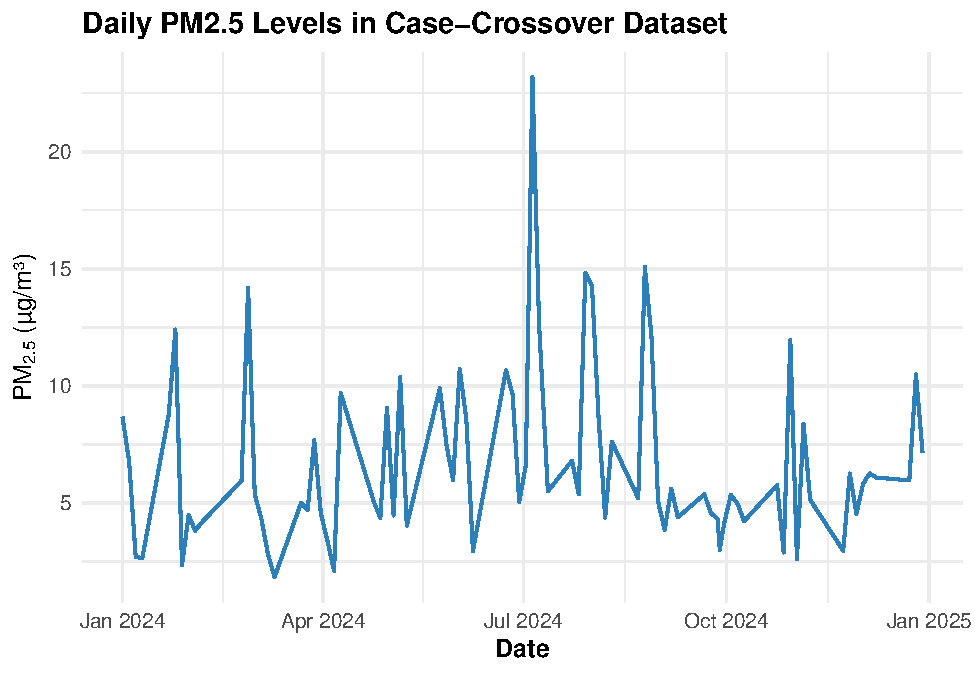
\includegraphics[keepaspectratio]{Preliminary-results_files/figure-latex/unnamed-chunk-56-1.pdf}}

\begin{Shaded}
\begin{Highlighting}[]
\CommentTok{\#Mental health outcome time series}
\FunctionTok{ggplot}\NormalTok{(df\_cc, }\FunctionTok{aes}\NormalTok{(}\AttributeTok{x =}\NormalTok{ date, }\AttributeTok{y =}\NormalTok{ mental\_health)) }\SpecialCharTok{+}
  \FunctionTok{geom\_line}\NormalTok{(}\AttributeTok{color =} \StringTok{"\#D95F02"}\NormalTok{, }\AttributeTok{linewidth =} \FloatTok{0.7}\NormalTok{) }\SpecialCharTok{+}
  \FunctionTok{labs}\NormalTok{(}
    \AttributeTok{title =} \StringTok{"Daily Mental Health EMS Calls"}\NormalTok{,}
    \AttributeTok{x =} \StringTok{"Date"}\NormalTok{,}
    \AttributeTok{y =} \StringTok{"Number of Calls"}
\NormalTok{  ) }\SpecialCharTok{+}
  \FunctionTok{theme\_minimal}\NormalTok{(}\AttributeTok{base\_size =} \DecValTok{12}\NormalTok{) }\SpecialCharTok{+}
  \FunctionTok{theme}\NormalTok{(}
    \AttributeTok{plot.title =} \FunctionTok{element\_text}\NormalTok{(}\AttributeTok{face =} \StringTok{"bold"}\NormalTok{),}
    \AttributeTok{axis.title =} \FunctionTok{element\_text}\NormalTok{(}\AttributeTok{face =} \StringTok{"bold"}\NormalTok{)}
\NormalTok{  )}
\end{Highlighting}
\end{Shaded}

\pandocbounded{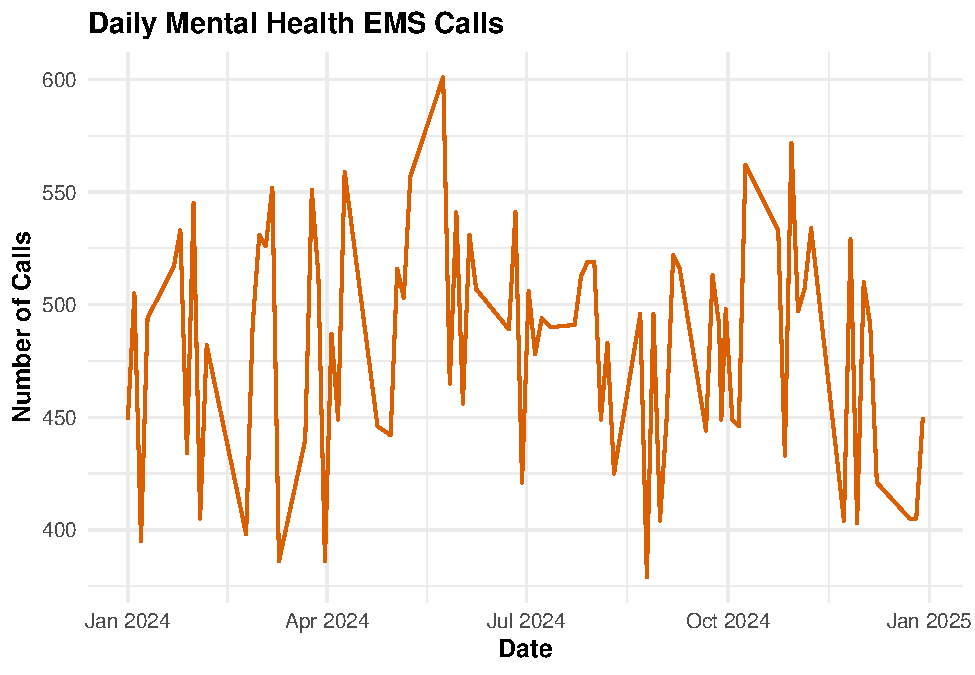
\includegraphics[keepaspectratio]{Preliminary-results_files/figure-latex/unnamed-chunk-57-1.pdf}}

\begin{Shaded}
\begin{Highlighting}[]
\CommentTok{\#Suicide outcome time series}
\FunctionTok{ggplot}\NormalTok{(df\_cc, }\FunctionTok{aes}\NormalTok{(}\AttributeTok{x =}\NormalTok{ date, }\AttributeTok{y =}\NormalTok{ suicide)) }\SpecialCharTok{+}
  \FunctionTok{geom\_line}\NormalTok{(}\AttributeTok{color =} \StringTok{"\#7570B3"}\NormalTok{, }\AttributeTok{linewidth =} \FloatTok{0.7}\NormalTok{) }\SpecialCharTok{+}
  \FunctionTok{labs}\NormalTok{(}
    \AttributeTok{title =} \StringTok{"Daily Suicide{-}Related EMS Calls"}\NormalTok{,}
    \AttributeTok{x =} \StringTok{"Date"}\NormalTok{,}
    \AttributeTok{y =} \StringTok{"Number of Calls"}
\NormalTok{  ) }\SpecialCharTok{+}
  \FunctionTok{theme\_minimal}\NormalTok{(}\AttributeTok{base\_size =} \DecValTok{12}\NormalTok{) }\SpecialCharTok{+}
  \FunctionTok{theme}\NormalTok{(}
    \AttributeTok{plot.title =} \FunctionTok{element\_text}\NormalTok{(}\AttributeTok{face =} \StringTok{"bold"}\NormalTok{),}
    \AttributeTok{axis.title =} \FunctionTok{element\_text}\NormalTok{(}\AttributeTok{face =} \StringTok{"bold"}\NormalTok{)}
\NormalTok{  )}
\end{Highlighting}
\end{Shaded}

\pandocbounded{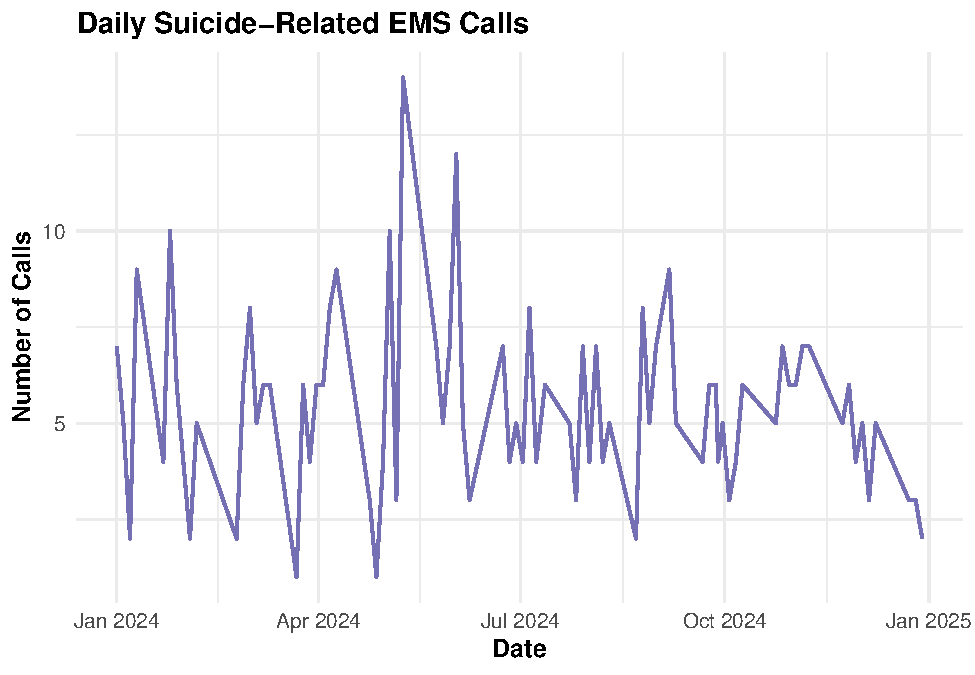
\includegraphics[keepaspectratio]{Preliminary-results_files/figure-latex/unnamed-chunk-58-1.pdf}}

\begin{Shaded}
\begin{Highlighting}[]
\CommentTok{\#Monthly average PM2.5}
\NormalTok{df\_pm25\_month }\OtherTok{\textless{}{-}}\NormalTok{ df\_cc }\SpecialCharTok{\%\textgreater{}\%}
  \FunctionTok{mutate}\NormalTok{(}\AttributeTok{month =} \FunctionTok{floor\_date}\NormalTok{(date, }\StringTok{"month"}\NormalTok{)) }\SpecialCharTok{\%\textgreater{}\%}
  \FunctionTok{group\_by}\NormalTok{(month) }\SpecialCharTok{\%\textgreater{}\%}
  \FunctionTok{summarise}\NormalTok{(}\AttributeTok{mean\_pm25 =} \FunctionTok{mean}\NormalTok{(pm25, }\AttributeTok{na.rm =} \ConstantTok{TRUE}\NormalTok{), }\AttributeTok{.groups =} \StringTok{"drop"}\NormalTok{)}

\FunctionTok{ggplot}\NormalTok{(df\_pm25\_month, }\FunctionTok{aes}\NormalTok{(}\AttributeTok{x =}\NormalTok{ month, }\AttributeTok{y =}\NormalTok{ mean\_pm25)) }\SpecialCharTok{+}
  \FunctionTok{geom\_line}\NormalTok{(}\AttributeTok{color =} \StringTok{"\#1B9E77"}\NormalTok{, }\AttributeTok{linewidth =} \FloatTok{0.8}\NormalTok{) }\SpecialCharTok{+}
  \FunctionTok{geom\_point}\NormalTok{(}\AttributeTok{color =} \StringTok{"\#1B9E77"}\NormalTok{, }\AttributeTok{size =} \DecValTok{2}\NormalTok{) }\SpecialCharTok{+}
  \FunctionTok{labs}\NormalTok{(}
    \AttributeTok{title =} \StringTok{"Monthly Average PM2.5"}\NormalTok{,}
    \AttributeTok{x =} \StringTok{"Month"}\NormalTok{,}
    \AttributeTok{y =} \FunctionTok{expression}\NormalTok{(}\StringTok{"Mean PM"}\NormalTok{[}\FloatTok{2.5}\NormalTok{] }\SpecialCharTok{*} \StringTok{" ("} \SpecialCharTok{*}\NormalTok{ mu }\SpecialCharTok{*} \StringTok{"g/"} \SpecialCharTok{*}\NormalTok{ m}\SpecialCharTok{\^{}}\DecValTok{3} \SpecialCharTok{*} \StringTok{")"}\NormalTok{)}
\NormalTok{  ) }\SpecialCharTok{+}
  \FunctionTok{theme\_minimal}\NormalTok{(}\AttributeTok{base\_size =} \DecValTok{12}\NormalTok{) }\SpecialCharTok{+}
  \FunctionTok{theme}\NormalTok{(}
    \AttributeTok{plot.title =} \FunctionTok{element\_text}\NormalTok{(}\AttributeTok{face =} \StringTok{"bold"}\NormalTok{),}
    \AttributeTok{axis.title =} \FunctionTok{element\_text}\NormalTok{(}\AttributeTok{face =} \StringTok{"bold"}\NormalTok{)}
\NormalTok{  )}
\end{Highlighting}
\end{Shaded}

\pandocbounded{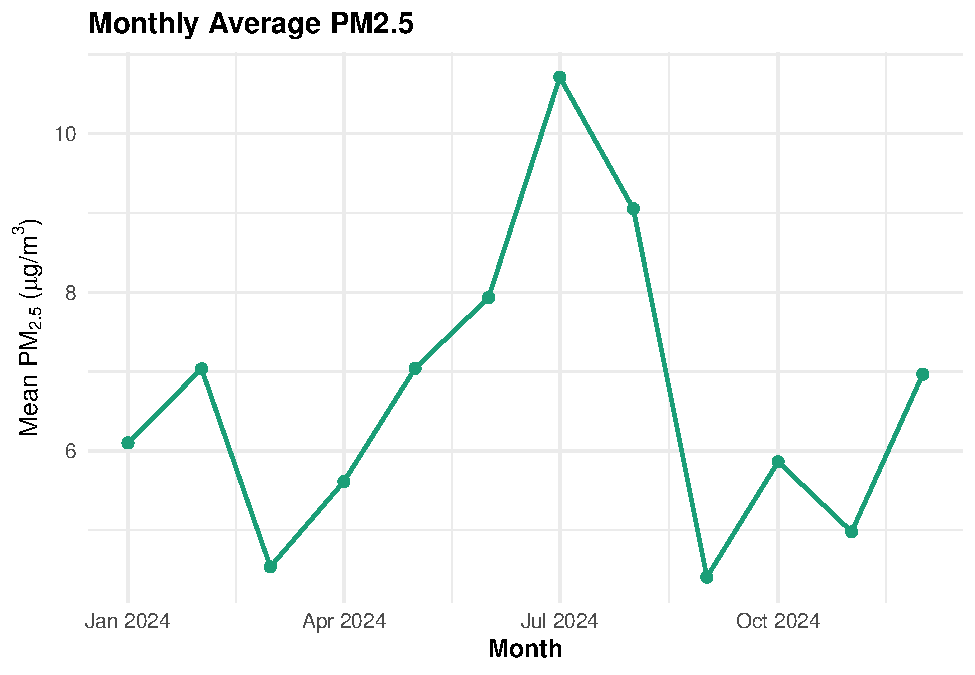
\includegraphics[keepaspectratio]{Preliminary-results_files/figure-latex/unnamed-chunk-59-1.pdf}}

\begin{Shaded}
\begin{Highlighting}[]
\CommentTok{\#PM2.5 by heat day}
\FunctionTok{ggplot}\NormalTok{(df\_cc, }\FunctionTok{aes}\NormalTok{(}\AttributeTok{x =} \FunctionTok{factor}\NormalTok{(heat\_day), }\AttributeTok{y =}\NormalTok{ pm25)) }\SpecialCharTok{+}
  \FunctionTok{geom\_boxplot}\NormalTok{(}\AttributeTok{fill =} \StringTok{"\#A6CEE3"}\NormalTok{) }\SpecialCharTok{+}
  \FunctionTok{labs}\NormalTok{(}
    \AttributeTok{title =} \StringTok{"Distribution of PM2.5 by Heat Day"}\NormalTok{,}
    \AttributeTok{x =} \StringTok{"Heat Day"}\NormalTok{,}
    \AttributeTok{y =} \FunctionTok{expression}\NormalTok{(}\StringTok{"PM"}\NormalTok{[}\FloatTok{2.5}\NormalTok{] }\SpecialCharTok{*} \StringTok{" ("} \SpecialCharTok{*}\NormalTok{ mu }\SpecialCharTok{*} \StringTok{"g/"} \SpecialCharTok{*}\NormalTok{ m}\SpecialCharTok{\^{}}\DecValTok{3} \SpecialCharTok{*} \StringTok{")"}\NormalTok{)}
\NormalTok{  ) }\SpecialCharTok{+}
  \FunctionTok{scale\_x\_discrete}\NormalTok{(}\AttributeTok{labels =} \FunctionTok{c}\NormalTok{(}\StringTok{"0"} \OtherTok{=} \StringTok{"No"}\NormalTok{, }\StringTok{"1"} \OtherTok{=} \StringTok{"Yes"}\NormalTok{)) }\SpecialCharTok{+}
  \FunctionTok{theme\_minimal}\NormalTok{(}\AttributeTok{base\_size =} \DecValTok{12}\NormalTok{) }\SpecialCharTok{+}
  \FunctionTok{theme}\NormalTok{(}
    \AttributeTok{plot.title =} \FunctionTok{element\_text}\NormalTok{(}\AttributeTok{face =} \StringTok{"bold"}\NormalTok{),}
    \AttributeTok{axis.title =} \FunctionTok{element\_text}\NormalTok{(}\AttributeTok{face =} \StringTok{"bold"}\NormalTok{)}
\NormalTok{  )}
\end{Highlighting}
\end{Shaded}

\pandocbounded{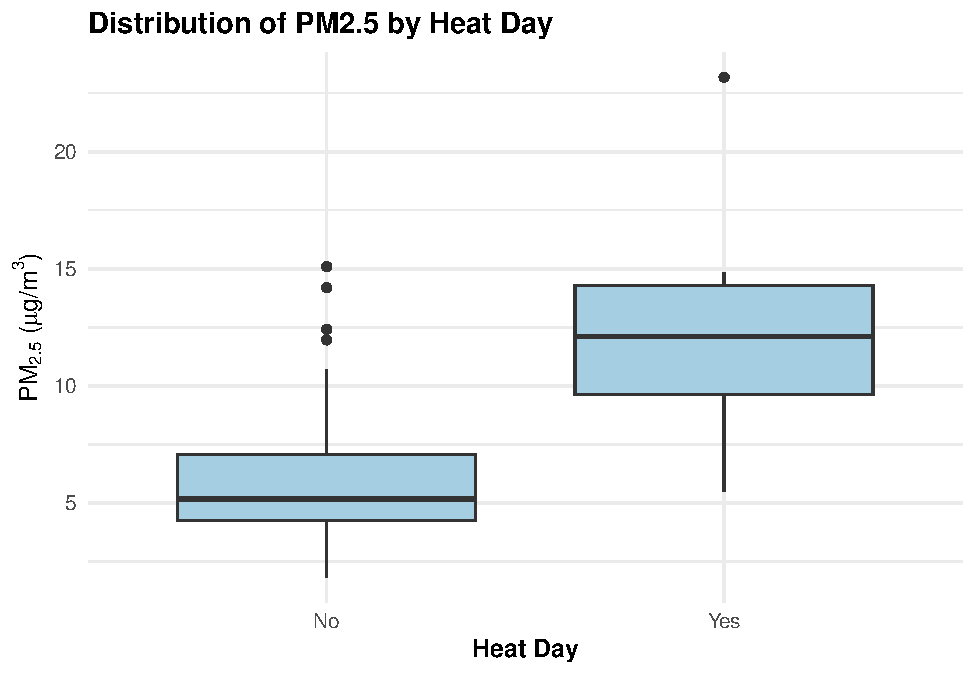
\includegraphics[keepaspectratio]{Preliminary-results_files/figure-latex/unnamed-chunk-60-1.pdf}}

\begin{Shaded}
\begin{Highlighting}[]
\CommentTok{\#Mental health calls by heat day}
\FunctionTok{ggplot}\NormalTok{(df\_cc, }\FunctionTok{aes}\NormalTok{(}\AttributeTok{x =} \FunctionTok{factor}\NormalTok{(heat\_day), }\AttributeTok{y =}\NormalTok{ mental\_health)) }\SpecialCharTok{+}
  \FunctionTok{geom\_boxplot}\NormalTok{(}\AttributeTok{fill =} \StringTok{"\#FDBF6F"}\NormalTok{) }\SpecialCharTok{+}
  \FunctionTok{labs}\NormalTok{(}
    \AttributeTok{title =} \StringTok{"Mental Health EMS Calls by Heat Day"}\NormalTok{,}
    \AttributeTok{x =} \StringTok{"Heat Day"}\NormalTok{,}
    \AttributeTok{y =} \StringTok{"Number of Calls"}
\NormalTok{  ) }\SpecialCharTok{+}
  \FunctionTok{scale\_x\_discrete}\NormalTok{(}\AttributeTok{labels =} \FunctionTok{c}\NormalTok{(}\StringTok{"0"} \OtherTok{=} \StringTok{"No"}\NormalTok{, }\StringTok{"1"} \OtherTok{=} \StringTok{"Yes"}\NormalTok{)) }\SpecialCharTok{+}
  \FunctionTok{theme\_minimal}\NormalTok{(}\AttributeTok{base\_size =} \DecValTok{12}\NormalTok{) }\SpecialCharTok{+}
  \FunctionTok{theme}\NormalTok{(}
    \AttributeTok{plot.title =} \FunctionTok{element\_text}\NormalTok{(}\AttributeTok{face =} \StringTok{"bold"}\NormalTok{),}
    \AttributeTok{axis.title =} \FunctionTok{element\_text}\NormalTok{(}\AttributeTok{face =} \StringTok{"bold"}\NormalTok{)}
\NormalTok{  )}
\end{Highlighting}
\end{Shaded}

\pandocbounded{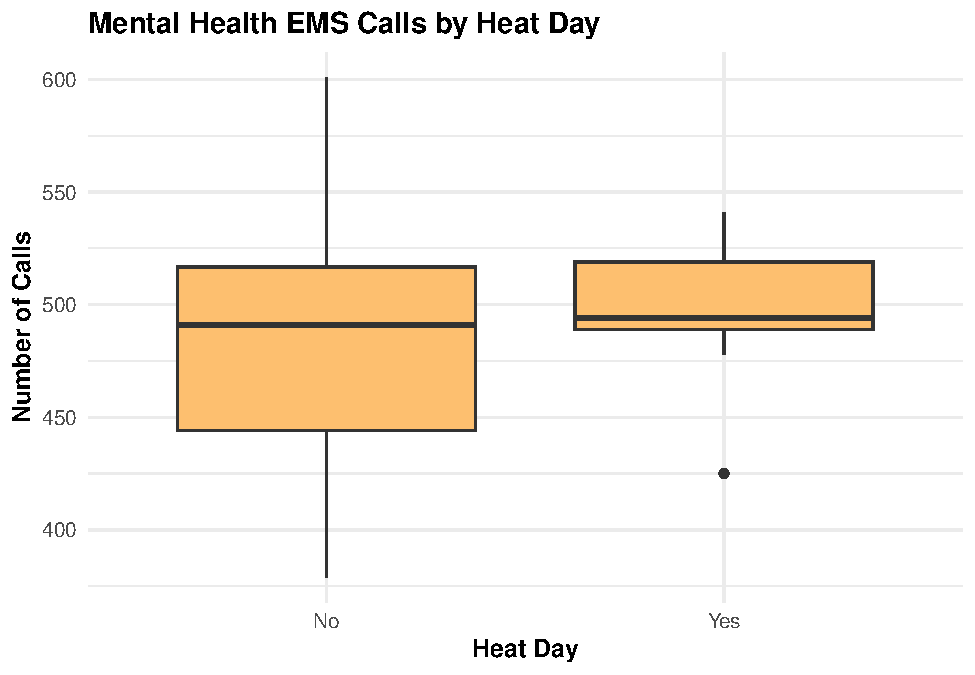
\includegraphics[keepaspectratio]{Preliminary-results_files/figure-latex/unnamed-chunk-61-1.pdf}}

\begin{Shaded}
\begin{Highlighting}[]
\CommentTok{\#Suicide calls by heat day}
\FunctionTok{ggplot}\NormalTok{(df\_cc, }\FunctionTok{aes}\NormalTok{(}\AttributeTok{x =} \FunctionTok{factor}\NormalTok{(heat\_day), }\AttributeTok{y =}\NormalTok{ suicide)) }\SpecialCharTok{+}
  \FunctionTok{geom\_boxplot}\NormalTok{(}\AttributeTok{fill =} \StringTok{"\#CAB2D6"}\NormalTok{) }\SpecialCharTok{+}
  \FunctionTok{labs}\NormalTok{(}
    \AttributeTok{title =} \StringTok{"Suicide{-}Related EMS Calls by Heat Day"}\NormalTok{,}
    \AttributeTok{x =} \StringTok{"Heat Day"}\NormalTok{,}
    \AttributeTok{y =} \StringTok{"Number of Calls"}
\NormalTok{  ) }\SpecialCharTok{+}
  \FunctionTok{scale\_x\_discrete}\NormalTok{(}\AttributeTok{labels =} \FunctionTok{c}\NormalTok{(}\StringTok{"0"} \OtherTok{=} \StringTok{"No"}\NormalTok{, }\StringTok{"1"} \OtherTok{=} \StringTok{"Yes"}\NormalTok{)) }\SpecialCharTok{+}
  \FunctionTok{theme\_minimal}\NormalTok{(}\AttributeTok{base\_size =} \DecValTok{12}\NormalTok{) }\SpecialCharTok{+}
  \FunctionTok{theme}\NormalTok{(}
    \AttributeTok{plot.title =} \FunctionTok{element\_text}\NormalTok{(}\AttributeTok{face =} \StringTok{"bold"}\NormalTok{),}
    \AttributeTok{axis.title =} \FunctionTok{element\_text}\NormalTok{(}\AttributeTok{face =} \StringTok{"bold"}\NormalTok{)}
\NormalTok{  )}
\end{Highlighting}
\end{Shaded}

\pandocbounded{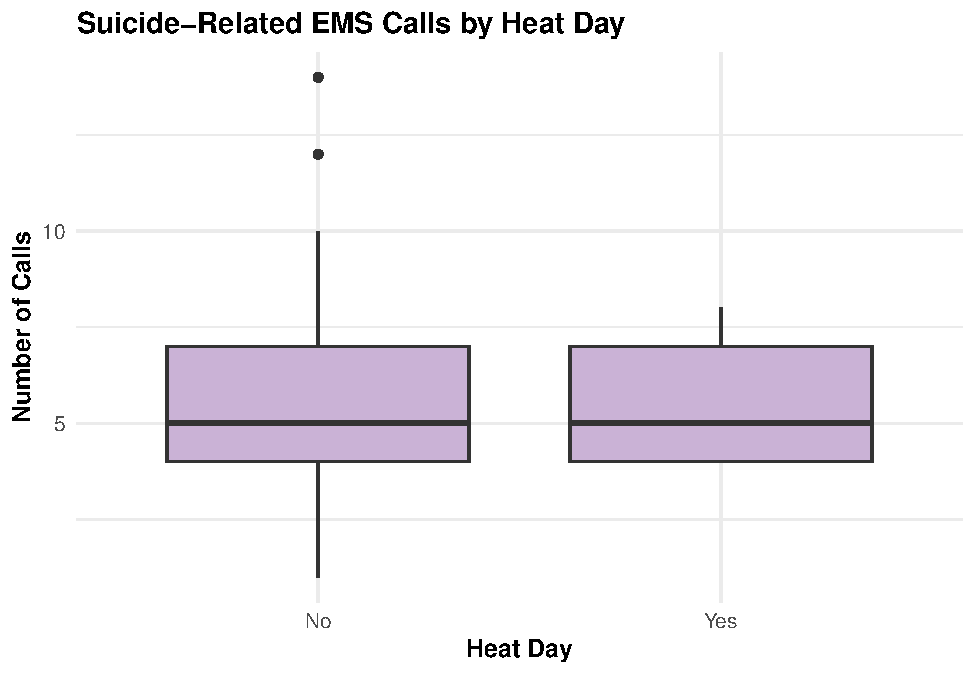
\includegraphics[keepaspectratio]{Preliminary-results_files/figure-latex/unnamed-chunk-62-1.pdf}}

\begin{Shaded}
\begin{Highlighting}[]
\NormalTok{irr\_plot\_data }\OtherTok{\textless{}{-}}\NormalTok{ irr\_results }\SpecialCharTok{\%\textgreater{}\%}
  \FunctionTok{filter}\NormalTok{(increment }\SpecialCharTok{==} \DecValTok{1}\NormalTok{) }\SpecialCharTok{\%\textgreater{}\%}
  \FunctionTok{mutate}\NormalTok{(}
    \AttributeTok{model\_label =} \FunctionTok{c}\NormalTok{(}
      \StringTok{"Mental health: lag 0"}\NormalTok{,}
      \StringTok{"Mental health: lag 0 + lag 1 (pm25)"}\NormalTok{,}
      \StringTok{"Mental health: lag 0 + lag 1 (pm25 lag1)"}\NormalTok{,}
      \StringTok{"Suicide: lag 0"}\NormalTok{,}
      \StringTok{"Suicide: lag 0 + lag 1 (pm25)"}\NormalTok{,}
      \StringTok{"Suicide: lag 0 + lag 1 (pm25 lag1)"}
\NormalTok{    )}
\NormalTok{  )}
\end{Highlighting}
\end{Shaded}

\begin{Shaded}
\begin{Highlighting}[]
\CommentTok{\#IRR forest plot}
\FunctionTok{ggplot}\NormalTok{(irr\_plot\_data, }\FunctionTok{aes}\NormalTok{(}\AttributeTok{x =}\NormalTok{ IRR, }\AttributeTok{y =} \FunctionTok{reorder}\NormalTok{(model\_label, IRR))) }\SpecialCharTok{+}
  \FunctionTok{geom\_point}\NormalTok{(}\AttributeTok{size =} \DecValTok{3}\NormalTok{, }\AttributeTok{color =} \StringTok{"\#1F78B4"}\NormalTok{) }\SpecialCharTok{+}
  \FunctionTok{geom\_errorbarh}\NormalTok{(}\FunctionTok{aes}\NormalTok{(}\AttributeTok{xmin =}\NormalTok{ CI\_low, }\AttributeTok{xmax =}\NormalTok{ CI\_high), }\AttributeTok{height =} \FloatTok{0.2}\NormalTok{, }\AttributeTok{color =} \StringTok{"\#1F78B4"}\NormalTok{) }\SpecialCharTok{+}
  \FunctionTok{geom\_vline}\NormalTok{(}\AttributeTok{xintercept =} \DecValTok{1}\NormalTok{, }\AttributeTok{linetype =} \StringTok{"dashed"}\NormalTok{, }\AttributeTok{color =} \StringTok{"red"}\NormalTok{) }\SpecialCharTok{+}
  \FunctionTok{labs}\NormalTok{(}
    \AttributeTok{title =} \StringTok{"IRRs for PM2.5 from Case{-}Crossover Models"}\NormalTok{,}
    \AttributeTok{x =} \StringTok{"Incidence Rate Ratio (95\% CI)"}\NormalTok{,}
    \AttributeTok{y =} \ConstantTok{NULL}
\NormalTok{  ) }\SpecialCharTok{+}
  \FunctionTok{theme\_minimal}\NormalTok{(}\AttributeTok{base\_size =} \DecValTok{12}\NormalTok{) }\SpecialCharTok{+}
  \FunctionTok{theme}\NormalTok{(}
    \AttributeTok{plot.title =} \FunctionTok{element\_text}\NormalTok{(}\AttributeTok{face =} \StringTok{"bold"}\NormalTok{)}
\NormalTok{  )}
\end{Highlighting}
\end{Shaded}

\pandocbounded{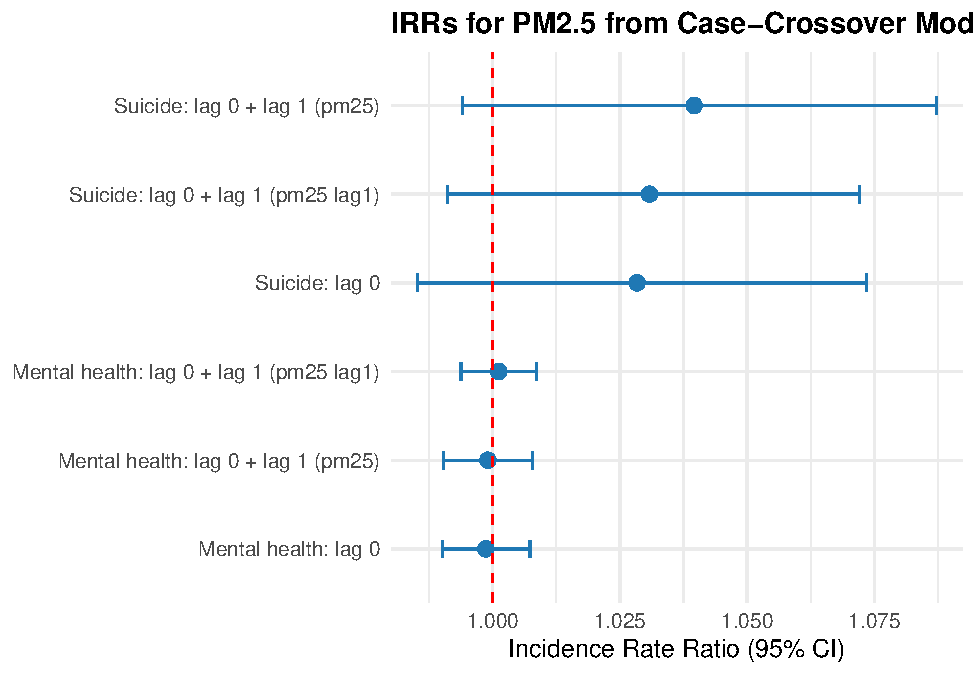
\includegraphics[keepaspectratio]{Preliminary-results_files/figure-latex/unnamed-chunk-64-1.pdf}}

\begin{Shaded}
\begin{Highlighting}[]
\CommentTok{\#Lag comparison plot for mental health}
\NormalTok{mh\_lag\_compare }\OtherTok{\textless{}{-}} \FunctionTok{bind\_rows}\NormalTok{(}
  \FunctionTok{get\_irr}\NormalTok{(m\_mh\_lag0, }\StringTok{"pm25"}\NormalTok{, }\DecValTok{1}\NormalTok{) }\SpecialCharTok{\%\textgreater{}\%} \FunctionTok{mutate}\NormalTok{(}\AttributeTok{model =} \StringTok{"Lag 0"}\NormalTok{),}
  \FunctionTok{get\_irr}\NormalTok{(m\_mh\_lag01, }\StringTok{"pm25"}\NormalTok{, }\DecValTok{1}\NormalTok{) }\SpecialCharTok{\%\textgreater{}\%} \FunctionTok{mutate}\NormalTok{(}\AttributeTok{model =} \StringTok{"Lag 0 + Lag 1"}\NormalTok{),}
  \FunctionTok{get\_irr}\NormalTok{(m\_mh\_lag012, }\StringTok{"pm25"}\NormalTok{, }\DecValTok{1}\NormalTok{) }\SpecialCharTok{\%\textgreater{}\%} \FunctionTok{mutate}\NormalTok{(}\AttributeTok{model =} \StringTok{"Lag 0 + Lag 1 + Lag 2"}\NormalTok{)}
\NormalTok{)}

\FunctionTok{ggplot}\NormalTok{(mh\_lag\_compare, }\FunctionTok{aes}\NormalTok{(}\AttributeTok{x =}\NormalTok{ IRR, }\AttributeTok{y =} \FunctionTok{reorder}\NormalTok{(model, IRR))) }\SpecialCharTok{+}
  \FunctionTok{geom\_point}\NormalTok{(}\AttributeTok{size =} \DecValTok{3}\NormalTok{, }\AttributeTok{color =} \StringTok{"\#33A02C"}\NormalTok{) }\SpecialCharTok{+}
  \FunctionTok{geom\_errorbarh}\NormalTok{(}\FunctionTok{aes}\NormalTok{(}\AttributeTok{xmin =}\NormalTok{ CI\_low, }\AttributeTok{xmax =}\NormalTok{ CI\_high), }\AttributeTok{height =} \FloatTok{0.2}\NormalTok{, }\AttributeTok{color =} \StringTok{"\#33A02C"}\NormalTok{) }\SpecialCharTok{+}
  \FunctionTok{geom\_vline}\NormalTok{(}\AttributeTok{xintercept =} \DecValTok{1}\NormalTok{, }\AttributeTok{linetype =} \StringTok{"dashed"}\NormalTok{, }\AttributeTok{color =} \StringTok{"red"}\NormalTok{) }\SpecialCharTok{+}
  \FunctionTok{labs}\NormalTok{(}
    \AttributeTok{title =} \StringTok{"Lag Structure Comparison for Mental Health Outcome"}\NormalTok{,}
    \AttributeTok{x =} \StringTok{"IRR for a 1{-}unit Increase in PM2.5"}\NormalTok{,}
    \AttributeTok{y =} \ConstantTok{NULL}
\NormalTok{  ) }\SpecialCharTok{+}
  \FunctionTok{theme\_minimal}\NormalTok{(}\AttributeTok{base\_size =} \DecValTok{12}\NormalTok{) }\SpecialCharTok{+}
  \FunctionTok{theme}\NormalTok{(}
    \AttributeTok{plot.title =} \FunctionTok{element\_text}\NormalTok{(}\AttributeTok{face =} \StringTok{"bold"}\NormalTok{)}
\NormalTok{  )}
\end{Highlighting}
\end{Shaded}

\pandocbounded{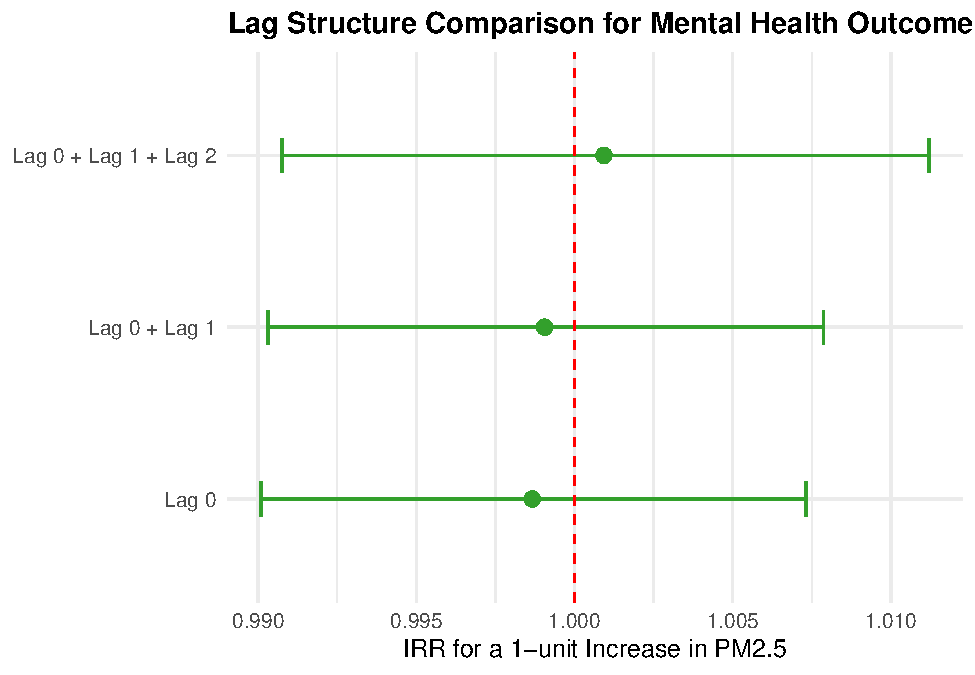
\includegraphics[keepaspectratio]{Preliminary-results_files/figure-latex/unnamed-chunk-65-1.pdf}}

\begin{Shaded}
\begin{Highlighting}[]
\CommentTok{\#Heat day interaction plot}
\NormalTok{df\_interaction\_plot }\OtherTok{\textless{}{-}}\NormalTok{ df\_cc }\SpecialCharTok{\%\textgreater{}\%}
  \FunctionTok{group\_by}\NormalTok{(heat\_day) }\SpecialCharTok{\%\textgreater{}\%}
  \FunctionTok{summarise}\NormalTok{(}
    \AttributeTok{mean\_pm25 =} \FunctionTok{mean}\NormalTok{(pm25, }\AttributeTok{na.rm =} \ConstantTok{TRUE}\NormalTok{),}
    \AttributeTok{mean\_mh =} \FunctionTok{mean}\NormalTok{(mental\_health, }\AttributeTok{na.rm =} \ConstantTok{TRUE}\NormalTok{),}
    \AttributeTok{.groups =} \StringTok{"drop"}
\NormalTok{  )}

\FunctionTok{ggplot}\NormalTok{(df\_interaction\_plot, }\FunctionTok{aes}\NormalTok{(}\AttributeTok{x =} \FunctionTok{factor}\NormalTok{(heat\_day), }\AttributeTok{y =}\NormalTok{ mean\_mh)) }\SpecialCharTok{+}
  \FunctionTok{geom\_col}\NormalTok{(}\AttributeTok{fill =} \StringTok{"\#FB9A99"}\NormalTok{) }\SpecialCharTok{+}
  \FunctionTok{labs}\NormalTok{(}
    \AttributeTok{title =} \StringTok{"Average Mental Health EMS Calls by Heat Day"}\NormalTok{,}
    \AttributeTok{x =} \StringTok{"Heat Day"}\NormalTok{,}
    \AttributeTok{y =} \StringTok{"Average Number of Calls"}
\NormalTok{  ) }\SpecialCharTok{+}
  \FunctionTok{scale\_x\_discrete}\NormalTok{(}\AttributeTok{labels =} \FunctionTok{c}\NormalTok{(}\StringTok{"0"} \OtherTok{=} \StringTok{"No"}\NormalTok{, }\StringTok{"1"} \OtherTok{=} \StringTok{"Yes"}\NormalTok{)) }\SpecialCharTok{+}
  \FunctionTok{theme\_minimal}\NormalTok{(}\AttributeTok{base\_size =} \DecValTok{12}\NormalTok{) }\SpecialCharTok{+}
  \FunctionTok{theme}\NormalTok{(}
    \AttributeTok{plot.title =} \FunctionTok{element\_text}\NormalTok{(}\AttributeTok{face =} \StringTok{"bold"}\NormalTok{),}
    \AttributeTok{axis.title =} \FunctionTok{element\_text}\NormalTok{(}\AttributeTok{face =} \StringTok{"bold"}\NormalTok{)}
\NormalTok{  )}
\end{Highlighting}
\end{Shaded}

\pandocbounded{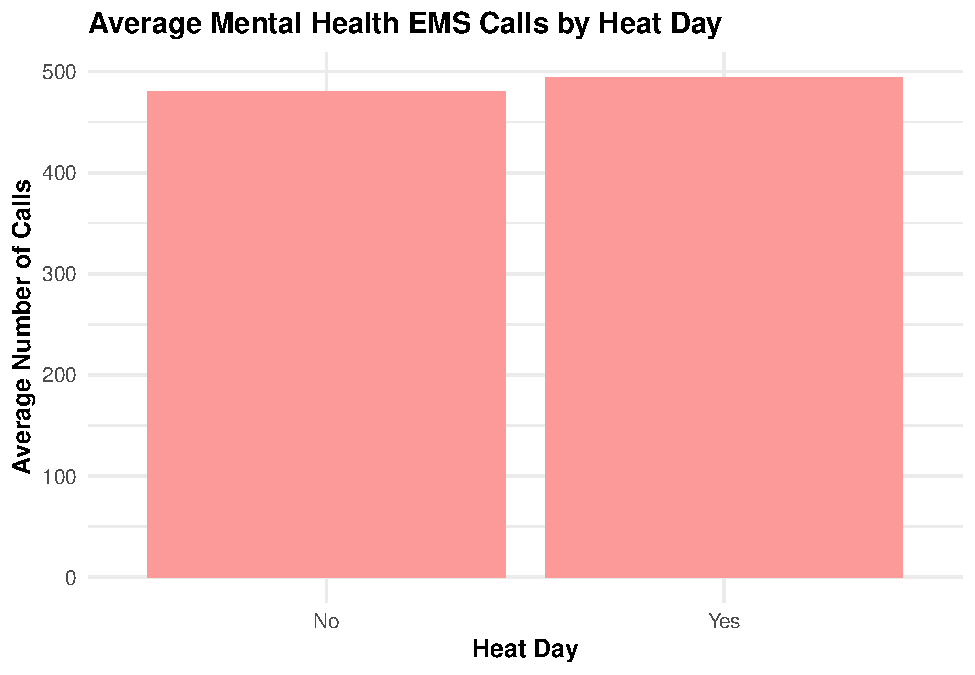
\includegraphics[keepaspectratio]{Preliminary-results_files/figure-latex/unnamed-chunk-66-1.pdf}}

\begin{Shaded}
\begin{Highlighting}[]
\NormalTok{final\_table }\OtherTok{\textless{}{-}}\NormalTok{ irr\_results }\SpecialCharTok{\%\textgreater{}\%}
  \FunctionTok{filter}\NormalTok{(increment }\SpecialCharTok{==} \DecValTok{1}\NormalTok{) }\SpecialCharTok{\%\textgreater{}\%}
  \FunctionTok{mutate}\NormalTok{(}
    \AttributeTok{Outcome =} \FunctionTok{case\_when}\NormalTok{(}
      \FunctionTok{grepl}\NormalTok{(}\StringTok{"mental"}\NormalTok{, model) }\SpecialCharTok{\textasciitilde{}} \StringTok{"Mental health"}\NormalTok{,}
      \FunctionTok{grepl}\NormalTok{(}\StringTok{"suicide"}\NormalTok{, model) }\SpecialCharTok{\textasciitilde{}} \StringTok{"Suicide"}
\NormalTok{    ),}
    \AttributeTok{Model =} \FunctionTok{case\_when}\NormalTok{(}
      \FunctionTok{grepl}\NormalTok{(}\StringTok{"lag012"}\NormalTok{, model) }\SpecialCharTok{\textasciitilde{}} \StringTok{"Lag 0–2"}\NormalTok{,}
      \FunctionTok{grepl}\NormalTok{(}\StringTok{"lag01"}\NormalTok{, model) }\SpecialCharTok{\&} \FunctionTok{grepl}\NormalTok{(}\StringTok{"lag1"}\NormalTok{, model) }\SpecialCharTok{\textasciitilde{}} \StringTok{"Lag 0–1 (lag 1 term)"}\NormalTok{,}
      \FunctionTok{grepl}\NormalTok{(}\StringTok{"lag01"}\NormalTok{, model) }\SpecialCharTok{\textasciitilde{}} \StringTok{"Lag 0–1 (lag 0 term)"}\NormalTok{,}
      \FunctionTok{grepl}\NormalTok{(}\StringTok{"lag0"}\NormalTok{, model) }\SpecialCharTok{\textasciitilde{}} \StringTok{"Lag 0"}
\NormalTok{    ),}
    \AttributeTok{IRR =} \FunctionTok{round}\NormalTok{(IRR, }\DecValTok{3}\NormalTok{),}
    \StringTok{\textasciigrave{}}\AttributeTok{95\% CI}\StringTok{\textasciigrave{}} \OtherTok{=} \FunctionTok{paste0}\NormalTok{(}\StringTok{"("}\NormalTok{, }\FunctionTok{round}\NormalTok{(CI\_low, }\DecValTok{3}\NormalTok{), }\StringTok{", "}\NormalTok{, }\FunctionTok{round}\NormalTok{(CI\_high, }\DecValTok{3}\NormalTok{), }\StringTok{")"}\NormalTok{)}
\NormalTok{  ) }\SpecialCharTok{\%\textgreater{}\%}
  \FunctionTok{select}\NormalTok{(Outcome, Model, IRR, }\StringTok{\textasciigrave{}}\AttributeTok{95\% CI}\StringTok{\textasciigrave{}}\NormalTok{) }\SpecialCharTok{\%\textgreater{}\%}
  \FunctionTok{as.data.frame}\NormalTok{()}

\FunctionTok{rownames}\NormalTok{(final\_table) }\OtherTok{\textless{}{-}} \ConstantTok{NULL}

\NormalTok{final\_table}
\end{Highlighting}
\end{Shaded}

\begin{verbatim}
##         Outcome                Model   IRR         95% CI
## 1 Mental health                Lag 0 0.999  (0.99, 1.007)
## 2 Mental health Lag 0–1 (lag 0 term) 0.999  (0.99, 1.008)
## 3 Mental health Lag 0–1 (lag 1 term) 1.001 (0.994, 1.009)
## 4       Suicide                Lag 0 1.028 (0.985, 1.073)
## 5       Suicide Lag 0–1 (lag 0 term) 1.040 (0.994, 1.087)
## 6       Suicide Lag 0–1 (lag 1 term) 1.031 (0.991, 1.072)
\end{verbatim}

\begin{Shaded}
\begin{Highlighting}[]
\NormalTok{knitr}\SpecialCharTok{::}\FunctionTok{kable}\NormalTok{(}
\NormalTok{  final\_table,}
  \AttributeTok{caption =} \StringTok{"Table 1. Case{-}crossover model results for PM2.5 and EMS outcomes"}
\NormalTok{)}
\end{Highlighting}
\end{Shaded}

\begin{longtable}[]{@{}llrl@{}}
\caption{Table 1. Case-crossover model results for PM2.5 and EMS
outcomes}\tabularnewline
\toprule\noalign{}
Outcome & Model & IRR & 95\% CI \\
\midrule\noalign{}
\endfirsthead
\toprule\noalign{}
Outcome & Model & IRR & 95\% CI \\
\midrule\noalign{}
\endhead
\bottomrule\noalign{}
\endlastfoot
Mental health & Lag 0 & 0.999 & (0.99, 1.007) \\
Mental health & Lag 0--1 (lag 0 term) & 0.999 & (0.99, 1.008) \\
Mental health & Lag 0--1 (lag 1 term) & 1.001 & (0.994, 1.009) \\
Suicide & Lag 0 & 1.028 & (0.985, 1.073) \\
Suicide & Lag 0--1 (lag 0 term) & 1.040 & (0.994, 1.087) \\
Suicide & Lag 0--1 (lag 1 term) & 1.031 & (0.991, 1.072) \\
\end{longtable}

Case-crossover preliminary results：

Using a time-stratified case-crossover design with conditional Poisson
regression, we examined the short-term association between PM2.5 and EMS
outcomes. For mental health-related EMS calls, the estimated IRRs were
close to 1 across lag 0 and lag 0--1 specifications, suggesting little
evidence of a strong short-term association in the preliminary analysis.
For suicide-related EMS calls, the point estimates were slightly above
1, but the confidence intervals still included 1, indicating that these
results were imprecise. Overall, the preliminary case-crossover results
did not show a clear association, but additional refinement of lag
structure and model specification will be explored in the final
analysis.

\end{document}
